% !TeX spellcheck = russian-aot-ieyo
% Зачем: Определяет класс документа (То, как будет выглядеть документ)
% Примечание: параметр draft помечает строки, вышедшие за границы страницы, прямоугольником, в фильной версии его нужно удалить.
\documentclass[a4paper,14pt,russian,oneside,final]{extreport}

% Зачем: Предоставляет проприетарный Times New Roman.
% ОБНОВЛЕНИЕ: лучше использовать scalable-cyrfonts-tex: меньше проблем с установкой
% Из руководства к PSCyr: "Во избежание проблем пакет PSCyr должен загружаться перед пакета-ми inputenc и babel".
% Примечание: Требует шаманства при установке, инструкция http://plumbum-blog.blogspot.com/2010/06/miktex-28-pscyr-04d.html
% http://blog.harrix.org/?p=444
% надо закомментировать это, чтобы использовать scalable-cyrfonts-tex:
\usepackage{pscyr}
\let\Tiny=\tiny

% Зачем: Предоставляет свободный Times New Roman.
% Шрифт идёт вместе с пакетом scalable-cyrfonts-tex в Ubuntu/Debian
% раскомментировать, чтобы использовать scalable-cyrfonts-tex:
%\usefont{T2A}{ftm}{m}{sl}

\usepackage{placeins}

% Зачем: Установка кодировки исходных файлов.
\usepackage[utf8]{inputenc}

% Зачем: Делает результирующий PDF "searchable and copyable".
\usepackage{cmap}

% Зачем: Выбор внутренней TeX кодировки.
\usepackage[T2A]{fontenc}

% Зачем: Чтобы можно было использовать русские буквы в формулах, но в случае использования предупреждать об этом.
\usepackage[warn]{mathtext}

% Зачем: Учет особенностей различных языков.
\usepackage[russian]{babel}

% Зачем: Добавляет поддержу дополнительных размеров текста 8pt, 9pt, 10pt, 11pt, 12pt, 14pt, 17pt, and 20pt.
% Почему: Пункт 2.1.1 Требований по оформлению пояснительной записки.
\usepackage{extsizes}

\sloppy
% Зачем: Длинна, пимерно соответвующая 5 символам
% Почему: Требования содержат странное требование про отсупы в 5 символов (для немоноширинного шрифта :| )
\newlength{\fivecharsapprox}
\setlength{\fivecharsapprox}{6ex}


\usepackage{afterpage}

% Зачем: Добавляет отступы для абзацев.
% Почему: Пункт 2.1.3 Требований по оформлению пояснительной записки.
\usepackage{indentfirst}
\setlength{\parindent}{\fivecharsapprox} % Примерно соответсвует 5 символам.


% Зачем: Настраивает отступы от границ страницы.
% Почему: Пункт 2.1.2 Требований по оформлению пояснительной записки.
\usepackage[left=3cm,top=2.0cm,right=1.5cm,bottom=2.7cm]{geometry}


% Зачем: Настраивает межстрочный интервал, для размещения 40 +/- 3 строки текста на странице.
% Почему: Пункт 2.1.1 Требований по оформлению пояснительной записки.
\usepackage[nodisplayskipstretch]{setspace}
\setstretch{1.1}
%\onehalfspacing

% Зачем: Выбор шрифта по-умолчанию.
% Почему: Пункт 2.1.1 Требований по оформлению пояснительной записки.
% Примечание: В требованиях не указан, какой именно шрифт использовать. По традиции используем TNR.
\renewcommand{\rmdefault}{ftm} % Times New Roman


% Зачем: Отключает использование изменяемых межсловных пробелов.
% Почему: Так не принято делать в текстах на русском языке.
\frenchspacing


% Зачем: Сброс счетчика сносок для каждой страницы
% Примечание: в "Требованиях по оформлению пояснительной записки" не указано, как нужно делать, но в других БГУИРовских докуметах рекомендуется нумерация отдельная для каждой страницы
\usepackage{perpage}
\MakePerPage{footnote}


% Зачем: Добавляет скобку 1) к номеру сноски
% Почему: Пункты 2.9.2 и 2.9.1 Требований по оформлению пояснительной записки.
\makeatletter
\def\@makefnmark{\hbox{\@textsuperscript{\normalfont\@thefnmark)}}}
\makeatother


% Зачем: Расположение сносок внизу страницы
% Почему: Пункт 2.9.2 Требований по оформлению пояснительной записки.
\usepackage[bottom]{footmisc}


% Зачем: Переопределяем стандартную нумерацию, т.к. в отчете будут только section и т.д. в терминологии TeX
\makeatletter
% Зачем: Переопределяем стандартную нумерацию, т.к. в отчете будут только section и т.д. в терминологии TeX
\renewcommand{\thesection}{\arabic{section}}


% Зачем: Для определения разных стилей (под)разделов в содержании и в тексте.
\usepackage{titlesec}

% Зачем: Начинаем разделы с новой страницы
\newcommand{\sectionbreak}{\clearpage}



\makeatother


% Зачем: Пункты (в терминологии требований) в терминологии TeX subsubsection должны нумероваться
% Почему: Пункт 2.2.3 Требований по оформлению пояснительной записки.
\setcounter{secnumdepth}{3}
\setcounter{tocdepth}{3}


% Зачем: Настраивает отступ между таблицей с содержанимем и словом СОДЕРЖАНИЕ
% Почему: Пункт 2.2.7 Требований по оформлению пояснительной записки.
\usepackage{tocloft}
\setlength{\cftbeforetoctitleskip}{-1em}
\setlength{\cftaftertoctitleskip}{1em}

% Зачем: Определяет отступы слева для записей в таблице содержания.
% Почему: Пункт 2.2.7 Требований по оформлению пояснительной записки.
\makeatletter
\renewcommand{\l@section}{\@dottedtocline{1}{0.5em}{1.2em}}
\renewcommand{\l@subsection}{\@dottedtocline{2}{1.7em}{2.0em}}
\renewcommand{\l@subsubsection}{\@dottedtocline{2}{3.7em}{2.8em}}
% \renewcommand\@dotsep{2}
\makeatother

\usepackage{seqsplit}
% Зачем: Работа с колонтитулами
\usepackage{fancyhdr} % пакет для установки колонтитулов
\pagestyle{fancy} % смена стиля оформления страниц




% Зачем: Нумерация страниц располагается справа снизу страницы
% Почему: Пункт 2.2.8 Требований по оформлению пояснительной записки.
\fancyhf{} % очистка текущих значений
\fancyfoot[R]{\thepage} % установка верхнего колонтитула
\renewcommand{\footrulewidth}{0pt} % убрать разделительную линию внизу страницы
\renewcommand{\headrulewidth}{0pt} % убрать разделительную линию вверху страницы
\fancypagestyle{plain}{
    \fancyhf{}
    \rfoot{\thepage}}

\usepackage[absolute]{textpos}
\usepackage{lscape,lipsum}

\fancypagestyle{lscape}{%
\fancyhf{} % clear all header and footer fields
\fancyfoot[R] {%
\begin{textblock}{1}(13,1){\rotatebox{90}{\thepage}}\end{textblock}}
\renewcommand{\headrulewidth}{0pt}
\renewcommand{\footrulewidth}{0pt}}



% Зачем: Задает стиль заголовков раздела жирным шрифтом, прописными буквами, без точки в конце
% Почему: Пункты 2.1.1, 2.2.5, 2.2.6 и ПРИЛОЖЕНИЕ Л Требований по оформлению пояснительной записки.
\makeatletter
\titleformat{\section}
  {\filright\hyphenpenalty=10000\normalfont\large\bfseries}
  {\thesection}
  {1em \@plus 1ex \@minus .2ex}{\MakeUppercase}

\titlespacing{\section}
    {\parindent}{0em}{1em \@plus .2ex}
\makeatother


% Зачем: Задает стиль заголовков подразделов
% Почему: Пункты 2.1.1, 2.2.5 и ПРИЛОЖЕНИЕ Л Требований по оформлению пояснительной записки.
\makeatletter
\titleformat{\subsection}
  {\filright\hyphenpenalty=10000\normalfont\normalsize\bfseries}
  {\textbf{\thesubsection}}
  {1em \@plus 1ex \@minus .2ex}{}

\titlespacing{\subsection}
    {\parindent}{1em \@plus 1ex \@minus .2ex}{1em \@plus .2ex}
\makeatother


% Зачем: Задает стиль заголовков пунктов
% Почему: Пункты 2.1.1, 2.2.5 и ПРИЛОЖЕНИЕ Л Требований по оформлению пояснительной записки.
\makeatletter
\titleformat{\subsubsection}
  {\filright\hyphenpenalty=10000\normalfont\normalsize}
  {\textbf{\thesubsubsection}}
  {1em \@plus 1ex \@minus .2ex}{}

\titlespacing{\subsubsection}
    {\parindent}{1em \@plus 1ex \@minus .2ex}{0em}
\makeatother


% Зачем: для оформления введения и заключения, они должны быть выровнены по центру.
% Почему: Пункты 1.1.15 и 1.1.11 Требований по оформлению пояснительной записки.
\makeatletter
\newcommand\sectioncentered{%
  \clearpage\@startsection {section}{1}%
    {\z@}%
    {-1em \@plus -1ex \@minus -.2ex}%
    {1em \@plus .2ex}%
    {\centering\hyphenpenalty=10000\normalfont\large\bfseries\MakeUppercase}%
    }
\makeatother


% Зачем: Задает стиль библиографии
% Почему: Пункт 2.8.6 Требований по оформлению пояснительной записки.
\bibliographystyle{styles/belarus-specific-utf8gost780u}






% Зачем: Пакет для вставки картинок
% Примечание: Объяснение, зачем final - http://tex.stackexchange.com/questions/11004/why-does-the-image-not-appear
\usepackage[final]{graphicx}
\DeclareGraphicsExtensions{.pdf,.png,.jpg,.eps}


% Зачем: Директория в которой будет происходить поиск картинок
\graphicspath{{figures/}}


% Зачем: Добавление подписей к рисункам
\usepackage[nooneline]{caption}
\usepackage{subcaption}

% Зачем: чтобы работала \No в новых латехах
\DeclareRobustCommand{\No}{\ifmmode{\nfss@text{\textnumero}}\else\textnumero\fi}

% Зачем: поворот ячеек таблиц на 90 градусов
\usepackage{rotating}
\DeclareRobustCommand{\povernut}[1]{\begin{sideways}{#1}\end{sideways}}


% Зачем: когда в формулах много кириллических символов команда \text{} занимает много места
\DeclareRobustCommand{\x}[1]{\text{#1}}

% Зачем: Задание подписей, разделителя и нумерации частей рисунков
% Почему: Пункт 2.5.5 Требований по оформлению пояснительной записки.
\DeclareCaptionLabelFormat{stbfigure}{Рисунок #2}
\DeclareCaptionLabelFormat{stbtable}{Таблица #2}
\DeclareCaptionLabelSeparator{stb}{~--~}
\captionsetup{labelsep=stb}
\captionsetup[figure]{skip=20pt,labelformat=stbfigure,justification=centering}
\captionsetup[table]{format=hang,skip=0pt,labelformat=stbtable,justification=raggedright}
\renewcommand{\thesubfigure}{\asbuk{subfigure}}

% Зачем: Окружения для оформления формул
% Почему: Пункт 2.4.7 требований по оформлению пояснительной записки и специфические требования различных кафедр
% Пример использования смотри в course_content.tex, строка 5
\usepackage{calc}
\newlength{\lengthWordWhere}
\settowidth{\lengthWordWhere}{где}
\newenvironment{explanationx}
    {%
    %%% Следующие строки определяют специфические требования разных редакций стандартов. Раскоменнтируйте нужную строку
    %% стандартный абзац, СТП-01 2010
    %\begin{itemize}[leftmargin=0cm, itemindent=\parindent + \lengthWordWhere + \labelsep, labelsep=\labelsep]
    %% без отступа, СТП-01 2013
    \begin{itemize}[leftmargin=0cm, itemindent=\lengthWordWhere + \labelsep , labelsep=\labelsep]%
    \renewcommand\labelitemi{}%
    }
    {%
    %\\[\parsep]
    \end{itemize}
    }

% Старое окружение для "где". Сохранено для совместимости
\usepackage{tabularx}

\newenvironment{explanation}
    {
    %%% Следующие строки определяют специфические требования разных редакций стандартов. Раскоменнтируйте нужные 2 строки
    %% стандартный абзац, СТП-01 2010
    %\par
    %\tabularx{\textwidth-\fivecharsapprox}{@{}ll@{ --- } X }
    %% без отступа, СТП-01 2013
    \noindent
    \tabularx{\textwidth}{@{}ll@{ --- } X }
    }
    {
    \\[\parsep]
    \endtabularx
    }


% Зачем: Удобная вёрстка многострочных формул, масштабирующийся текст в формулах, формулы в рамках и др
\usepackage{amsmath}

\usepackage{lscape}


% Зачем: Поддержка ажурного и готического шрифтов
\usepackage{amsfonts}


% Зачем: amsfonts + несколько сотен дополнительных математических символов
\usepackage{amssymb}


% Зачем: Окружения «теорема», «лемма»
\usepackage{amsthm}


% Зачем: Производить арифметические операции во время компиляции TeX файла
\usepackage{calc}

% Зачем: Производить арифметические операции во время компиляции TeX файла
\usepackage{fp}

% Зачем: Пакет для работы с перечислениями
\usepackage{enumitem}
\makeatletter
 \AddEnumerateCounter{\asbuk}{\@asbuk}{щ)}
\makeatother


% Зачем: Устанавливает символ начала простого перечисления
% Почему: Пункт 2.3.5 Требований по оформлению пояснительной записки.
\setlist{nolistsep}


% Зачем: Устанавливает символ начала именованного перечисления
% Почему: Пункт 2.3.8 Требований по оформлению пояснительной записки.
\renewcommand{\labelenumi}{\asbuk{enumi})}
\renewcommand{\labelenumii}{\arabic{enumii})}

% Зачем: Устанавливает отступ от границы документа до символа списка, чтобы этот отступ равнялся отступу параграфа
% Почему: Пункт 2.3.5 Требований по оформлению пояснительной записки.

\setlist[itemize,0]{itemindent=\parindent + 2.2ex,leftmargin=0ex,label=--}
\setlist[enumerate,1]{itemindent=\parindent + 2.7ex,leftmargin=0ex}
\setlist[enumerate,2]{itemindent=\parindent + \parindent - 2.7ex}

% Зачем: Включение номера раздела в номер формулы. Нумерация формул внутри раздела.
\AtBeginDocument{\numberwithin{equation}{section}}

% Зачем: Включение номера раздела в номер таблицы. Нумерация таблиц внутри раздела.
\AtBeginDocument{\numberwithin{table}{section}}

% Зачем: Включение номера раздела в номер рисунка. Нумерация рисунков внутри раздела.
\AtBeginDocument{\numberwithin{figure}{section}}


% Зачем: Дополнительные возможности в форматировании таблиц
\usepackage{makecell}
\usepackage{multirow}
\usepackage{array}


% Зачем: "Умная" запятая в математических формулах. В дробных числах не добавляет пробел
% Почему: В требованиях не нашел, но в русском языке для дробных чисел используется {,} а не {.}
\usepackage{icomma}

% Зачем: макрос для печати римских чисел
\makeatletter
\newcommand{\rmnum}[1]{\romannumeral #1}
\newcommand{\Rmnum}[1]{\expandafter\@slowromancap\romannumeral #1@}
\makeatother


% Зачем: Управление выводом чисел.
\usepackage{sistyle}
\SIdecimalsign{,}

% Зачем: inline-коментирование содержимого.
\newcommand{\ignore}[2]{\hspace{0in}#2}


% Зачем: Возможность коментировать большие участки документа
\usepackage{verbatim}


\usepackage{xcolor}


% Зачем: Оформление листингов кода
% Примечание: final нужен для переопределения режима draft, в котором листинги не выводятся в документ.
\usepackage[final]{listings}


% Зачем: настройка оформления листинга для языка F#
\definecolor{bluekeywords}{rgb}{0.13,0.13,1}
\definecolor{greencomments}{rgb}{0,0.5,0}
\definecolor{turqusnumbers}{rgb}{0.17,0.57,0.69}
\definecolor{redstrings}{rgb}{0.5,0,0}

\renewcommand{\lstlistingname}{Листинг}

\lstdefinelanguage{FSharp}
    {morekeywords={abstract,and,as,assert,base,begin,class,default,delegate,do,done,downcast,downto,elif,else,end,exception,extern,false,finally,for,fun,function,global,if,in,inherit,inline,interface,internal,lazy,let,let!,match,member,module,mutable,namespace,new,not,null,of,open,or,override,private,public,rec,return,return!,select,static,struct,then,to,true,try,type,upcast,use,use!,val,void,when,while,with,yield,yield!,asr,land,lor,lsl,lsr,lxor,mod,sig,atomic,break,checked,component,const,constraint,constructor,continue,eager,event,external,fixed,functor,include,method,mixin,object,parallel,process,protected,pure,sealed,tailcall,trait,virtual,volatile},
    keywordstyle=\bfseries\color{bluekeywords},
    sensitive=false,
    morecomment=[l][\color{greencomments}]{///},
    morecomment=[l][\color{greencomments}]{//},
    morecomment=[s][\color{greencomments}]{{(*}{*)}},
    morestring=[b]",
    stringstyle=\color{redstrings},
    }


\lstset{%
showstringspaces=false
escapechar=\&
}


\lstdefinestyle{fsharpstyle}{
   xleftmargin=0ex,
   language=FSharp,
   basicstyle=\footnotesize\ttfamily,
   breaklines=true,
   columns=fullflexible
}
\lstdefinestyle{rubystyle} {
  language=Ruby,
  morekeywords={new},
  breaklines=true,
  columns=fullflexible,
  basicstyle=\footnotesize\ttfamily,
  commentstyle = \ttfamily\color{gray},
  keywordstyle=\ttfamily\color{black},
  stringstyle=\color{black}
}


\lstdefinestyle{csharpinlinestyle} {
  language=[Sharp]C,
  morekeywords={yield,var,get,set,from,select,partial,where,async,await},
  breaklines=true,
  columns=fullflexible,
  basicstyle=\footnotesize\ttfamily
}

\lstdefinestyle{csharpstyle}{
  language=[Sharp]C,
  frame=lr,
  rulecolor=\color{blue!80!black}}


% Зачем: Нумерация листингов в пределах секции
\AtBeginDocument{\numberwithin{lstlisting}{section}}

\usepackage[normalem]{ulem}

\usepackage[final,hidelinks]{hyperref}
% Моноширинный шрифт выглядит визуально больше, чем пропорциональный шрифт, если их размеры одинаковы. Искусственно уменьшаем размер ссылок.
\renewcommand{\UrlFont}{\small\rmfamily\tt}

\usepackage[square,numbers,sort&compress]{natbib}
\setlength{\bibsep}{0em}

% Магия для подсчета разнообразных объектов в документе
\usepackage{lastpage}
\usepackage{totcount}
\regtotcounter{section}

\usepackage{etoolbox}

\newcounter{totfigures}
\newcounter{tottables}
\newcounter{totreferences}
\newcounter{totequation}

\providecommand\totfig{}
\providecommand\tottab{}
\providecommand\totref{}
\providecommand\toteq{}

\makeatletter
\AtEndDocument{%
  \addtocounter{totfigures}{\value{figure}}%
  \addtocounter{tottables}{\value{table}}%
  \addtocounter{totequation}{\value{equation}}
  \immediate\write\@mainaux{%
    \string\gdef\string\totfig{\number\value{totfigures}}%
    \string\gdef\string\tottab{\number\value{tottables}}%
    \string\gdef\string\totref{\number\value{totreferences}}%
    \string\gdef\string\toteq{\number\value{totequation}}%
  }%
}
\makeatother

\pretocmd{\section}{\addtocounter{totfigures}{\value{figure}}\setcounter{figure}{0}}{}{}
\pretocmd{\section}{\addtocounter{tottables}{\value{table}}\setcounter{table}{0}}{}{}
\pretocmd{\section}{\addtocounter{totequation}{\value{equation}}\setcounter{equation}{0}}{}{}
\pretocmd{\bibitem}{\addtocounter{totreferences}{1}}{}{}



% Для оформления таблиц не влязящих на 1 страницу
\usepackage{longtable}

% Для включения pdf документов в результирующий файл
\usepackage{pdfpages}

% Для использования знака градуса и других знаков
% http://ctan.org/pkg/gensymb
\usepackage{gensymb}

% Зачем: преобразовывать текст в верхний регистр командой MakeTextUppercase
\usepackage{textcase}

% Зачем: Переносы в словах с тире.
% Тире в словае заменяем на \hyph: аппаратно\hyphпрограммный.
% https://stackoverflow.com/questions/2193307/how-to-get-latex-to-hyphenate-a-word-that-contains-a-dash#
\def\hyph{-\penalty0\hskip0pt\relax}

% Добавляем абзацный отступ для библиографии
% https://github.com/mstyura/bsuir-diploma-latex/issues/19
\setlength\bibindent{-1.0900cm}

\makeatletter
\renewcommand\NAT@bibsetnum[1]{\settowidth\labelwidth{\@biblabel{#1}}%
   \setlength{\leftmargin}{\bibindent}\addtolength{\leftmargin}{\dimexpr\labelwidth+\labelsep\relax}%
   \setlength{\itemindent}{-\bibindent+\fivecharsapprox-0.240cm}%
   \setlength{\listparindent}{\itemindent}
\setlength{\itemsep}{\bibsep}\setlength{\parsep}{\z@}%
   \ifNAT@openbib
     \addtolength{\leftmargin}{\bibindent}%
     \setlength{\itemindent}{-\bibindent}%
     \setlength{\listparindent}{\itemindent}%
     \setlength{\parsep}{10pt}%
   \fi
}



\newcommand{\csharp}{C\#}
\newcommand{\fsharp}{F\#}
\newcommand{\vbnet}{Visual Basic~.NET}
\newcommand{\cpp}{C\texttt{\hspace{-0.3ex}+\hspace{-0.25ex}+}}
\newcommand{\cppcli}{Visual \cpp{}/CLI}
\newcommand{\dotnet}{Microsoft .NET}
\newcommand{\netfx}{.NET Framework}
\newcommand{\java}{Java}

\begin{document}

\begin{titlepage}
  \begin{center}
    Министерство образования Республики Беларусь\\[1em]
    Учреждение образования\\
    БЕЛОРУССКИЙ ГОСУДАРСТВЕННЫЙ УНИВЕРСИТЕТ \\
    ИНФОРМАТИКИ И РАДИОЭЛЕКТРОНИКИ\\[1em]

    \begin{minipage}{\textwidth}
      \begin{flushleft}
        \begin{tabular}{ l }
          Факультет компьютерных систем и сетей\\
          Кафедра программного обеспечения информационных технологий
        \end{tabular}
      \end{flushleft}
    \end{minipage}\\[1em]

    \begin{flushright}
      \begin{minipage}{0.4\textwidth}
        \textit{К защите допустить:}\\[0.8em]
        Заведующий кафедрой ПОИТ\\[0.45em]
        \underline{\hspace*{2.8cm}} Н.\,В.~Лапицкая
      \end{minipage}\\[2.2em]
    \end{flushright}

    %%
    %% ВНИМАНИЕ: на некторых факультетах (ФКП) и кафедрах (ПИКС) слова "ПОЯСНИТЕЛЬНАЯ ЗАПИСКА" предлагается (требуется) оформлять полужирным начертанием. Раскомментируйте нужную для вас строку:
    %%
    %\textbf{ПОЯСНИТЕЛЬНАЯ ЗАПИСКА}\\
    {ПОЯСНИТЕЛЬНАЯ ЗАПИСКА}\\
    {к дипломному проекту}\\
    {на тему}\\[1em]
    \textbf{\large ПРОГРАММНОЕ СРЕДСТВО WEB ПРИЛОЖЕНИЕ ДЛЯ ПРОДАЖИ КВАРТИР}\\[1em]


    {БГУИР ДП 1-40 01 01 03 *** ПЗ}\\[2em]

    \begin{tabular}{ p{0.65\textwidth}p{0.25\textwidth} }
      Студент & Е.\,М.~Новик \\
      Руководитель & Д.\,В.~Горбачев \\
      Консультанты: &\\
      \hspace*{3ex}\emph{от кафедры ПОИТ} & Д.\,В.~Горбачев \\
      \hspace*{3ex}\emph{по экономической части} & Е.\,В.~Анохин \\
      %%
      %% ВНИМАНИЕ: в зависимости от выбранной темы, у вас консультант может быть как по охране труда, так и по:
        % экологической безопасности
        % ресурсосбережению
        % энергосбережению
      %%
      %% Впишите правильную формулировку по необходимости
      Нормоконтролёр & В.\,А.~Леванцевич \\
      & \\
      Рецензент &
    \end{tabular}

    \vfill
    {\normalsize Минск 2017}
  \end{center}
\end{titlepage}
 % page 1

\sectioncentered*{Реферат}
\thispagestyle{empty}
%%
%% ВНИМАНИЕ: этот реферат не соответствует СТП-01 2013
%% пример оформления реферата смотрите здесь: http://www.bsuir.by/m/12_100229_1_91132.docx
%%


\begin{center}
Пояснительная записка \pageref*{LastPage}c., \totfig{}~рис., \tottab{}~табл., \toteq{}~формул и \totref{}~литературный источник.\\
ЗАПУТЫВАНИЕ, VHDL, ПАРСИНГ, ОБФУСКАЦИЯ, RTL
\end{center}

Предметной областью разработки является сфера защиты интеллектуальной собственности, анализа кодов и обфускации. Объект разработки -- приложение для конечного пользователя, предоставляющее функционал по анализу и запутыванию кода.

Целью разработки является создание удобного, простого приложения, пригодного для решения практических задач, возникающих при работе в области моделирования дизайнов на языке VHDL.

При разработке проекта использовалась среда разработки Sublime Text 3 с различными расширениями, такими как, LatexTools, Package Control и т.д. Язык программирования приложения -- Ruby.


Результатом разработки стало простое в использовании приложение, которое может быть легко интегрировано в процесс работы, предоставляющее различные возможности по проверке и запутыванию кода. Разработаны диаграмма компонентов, диаграмма потоков данных, а также различные схемы алгоритмов.

Предполагается использование приложения разработчиками цифровых микросхем.

Разработанное приложение является экономически эффективным, оно полностью  оправдывает средства, вложенные в его разработку.
% Дипломный проект выполнен на 6 листах формата А1 с пояснительной запиской на~\pageref*{LastPage} страницах, без приложений справочного или информационного характера.

% Целью дипломного проекта является разработка удобного в использовании инструмента, пригодного для решения практических задач, возникающих в реальных проектах, связанных с вероятностным моделированием.

% Для достижения цели дипломного проекта была разработана библиотека кода для \dotnet{}, предназначенная для представления и обучения структуры вероятностной сети по экспериментальным данным.
% Библиотека может быть использована в реальных проектах, использующих вероятностный подход к решению проблемы.
% В библиотеке реализовано несколько алгоритмов, имеющих различные качественные характеристики.

% В разделе технико"=экономического обоснования был произведён расчёт затрат на создание ПО, а также прибыли от разработки, получаемой разработчиком.
% Проведённые расчёты показали экономическую целесообразность проекта.

% Пояснительная записка включает раздел по охране труда, в котором была произведена оценка пожарной безопасности на предприятии, где частично разрабатывался данный дипломный проект.

\clearpage
 % page 2

%{
    % Вставка текста
    \newcommand{\lineunderscore}[1][]{%
        \uline{#1}\uline{\hspace*{\fill}}%
    }

    \newcommand{\lineunderscorec}[1][]{%
        \uline{\hspace*{\fill}}%
        \lineunderscore[#1]%
    }

    % Установка основного размера шрифта для страницы: 12pt
    \makeatletter\let\newcommand\renewcommand\input{size12.clo}

    \newgeometry{top=1.25cm,bottom=1.25cm,right=1cm,left=2cm,twoside}
    \thispagestyle{empty}
    \setlength{\parindent}{0em}


    \begin{center}
        Министерство образования Республики Беларусь\\
        Учреждение образования\\
        БЕЛОРУССКИЙ ГОСУДАРСТВЕННЫЙ УНИВЕРСИТЕТ \\
        ИНФОРМАТИКИ И РАДИОЭЛЕКТРОНИКИ\\[1em]

    \begin{minipage}{\textwidth}
        \begin{flushleft}
            \begin{tabular}{ p{0.20\textwidth}p{0.31\textwidth}p{0.20\textwidth}p{0.20\textwidth} @{} }
                Факультет & \lineunderscore[КСиС] & Кафедра & \lineunderscore[ПОИТ] \\
                Специальность & \lineunderscore[1-40 01 01] & Специализация & \lineunderscore[03]
            \end{tabular}
        \end{flushleft}
    \end{minipage}\\[1em]

    \begin{minipage}{\textwidth}
        \begin{flushright}
            \begin{tabular}{p{0.40\textwidth}}
                УТВЕРЖДАЮ \\[0.5em]
                \underline{\hspace*{7em}} Н.В.~Лапицкая \\
                <<\underline{\hspace*{4ex}}>> \underline{\hspace*{7em}} \the\year~г.
            \end{tabular}
        \end{flushright}
    \end{minipage}\\[1em]

    \textbf{ЗАДАНИЕ} \\
    \textbf{по дипломному проекту (работе) студента} \\
    \vspace{1em}
    \textbf{\lineunderscorec[Шадура Евгения Александровича]} \\
    {\small (фамилия, имя, отчество) }

    \end{center}

    1. Тема проекта (работы):
    \lineunderscore[Программное средство лексической и функциональной обфускации проектных описаний цифровых устройств]\\
    \lineunderscore\\
    утверждена приказом по университету от <<\uline{~~09~~}>> \uline{~~февраля~~} \the\year~г. \No{} \uline{~~265-c~~}

    \vspace{1em}

    2. Срок сдачи студентом законченного проекта (работы): \lineunderscorec[1 июня \the\year~года]

    \vspace{1em}

    3. Исходные данные к проекту (работе):
    \lineunderscore[Тип операционной системы~-- Windows, Linux; Языки программирования~-- Ruby, Перечень выполняемых функций: а) анализ исходного кода на языке VHDL; б) лексическая обфускация исходного кода; в) функциональная обфускация синтезируемой схемы; г) Интеграция с другими средами разработки. Назначение разработки: создание программного средства для лексической и функциональной обфускации проектных описаний, написанных на языке VHDL]

    \vspace{1em}

    4. Содержание пояснительной записки (перечень подлежащих разработке вопросов):
    \lineunderscore[Введение]\\
    \lineunderscore[1 Анализ литературы в области защиты интеллектуальных прав, пиратства, и обфускации кода]\\
    \lineunderscore[2 Используемые технологии]\\
    \lineunderscore[3 Проектирование архитектуры программного средства]\\
    \lineunderscore[4 Тестирование программного средства]\\
    \lineunderscore[5 Методика использования разработанного программного средства]\\
    \lineunderscore[6 Технико-экономическое обоснование эффективности разработки и использования
    программного средства]\\
    \lineunderscore[Заключение]\\
    \lineunderscore[Список использованных источников]\\
    \lineunderscore[Приложение А Исходный код программного средства]

    \clearpage
    \thispagestyle{empty}

    5. Перечень графического материала (с точным указанием обязательных чертежей):
    \lineunderscore[Исходный код и результат синтеза до обфускации и после. Плакат - формат А1, лист 1.]\\
    \lineunderscore[Диаграмма компонентов программного средства. Плакат - формат А1, лист 1.]\\
    \lineunderscore[Диаграмма потоков данных программного средства. Плакат - формат А1, лист 1.]\\
    \lineunderscore[Программное средство лексической и функциональной обфускации проектных описаний цифровых устройств. Схема программы - формат А1, лист 1.]\\
    \lineunderscore[Лексический анализатор. Схема алгоритма - формат А1, лист 1.]\\
    \lineunderscore[Обфускация исходного кода. Схема алгоритма - формат А1, лист 1.]\\
    \lineunderscore

    \vspace{1em}

    6. Содержание задания по технико-экономическому обоснованию:\\
    \lineunderscore[Расчет экономической эффективности от разработки программного средства лексической и функциональной обфускации проектных описаний цифровых устройств]\\
    \lineunderscore

    Задание выдал: \uline{\hspace*{6em}} / К.\,Р.~Литвинович /

    \vspace{1em}

    %\vfill

    \begin{center}
      \textbf{КАЛЕНДАРНЫЙ ПЛАН}
    \end{center}

    \begin{tabular}{
        | m{0.51\textwidth}
        | >{\centering}m{0.09\textwidth}
        | >{\centering}m{0.20\textwidth}
        | >{\centering\arraybackslash\hspace{0pt}}m{0.10\textwidth}|
    }
        \hline \centering{Наименование этапов дипломного проекта (работы)} & Объем этапа, \% & Срок выполнения этапов & Примечание \\
        \hline Анализ предметной области, & & & \\
        \hline разработка технического задания & 15-20\% & 01.02--14.02 & \\
        \hline Разработка функциональных требований, & & & \\
        \hline проектирование архитектуры программы & 15-20\% & 15.02--06.03 & \\
        \hline Разработка схемы программы, алгоритмов, & & & \\
        \hline схемы данных & 15-20\% & 07.03--27.03 & \\
        \hline Разработка программного средства & 15-20\% & 28.03--24.04 & \\
        \hline Тестирование и отладка & 10\% & 25.04--08.05 & \\
        \hline Оформление пояснительной записки & & & \\
        \hline и графического материала & 20\% & 09.05-31.05 & \\
        \hline
    \end{tabular}

    \vspace{2em}

    Дата выдачи задания \lineunderscorec[~~1 февраля 2016~~] \hspace{2ex} Руководитель \hfill{} \uline{\hspace*{4em}} / А.\,А.~Иванюк /

    \vspace{1em}

    Задание принял к исполнению  \uline{\hspace*{4em}} / Е.\,А.~Шадура /

    \restoregeometry
} % pages 3 and 4. printed separately

% \sectioncentered*{Аннотация}
\thispagestyle{empty}

\begin{center}
  \begin{minipage}{0.82\textwidth}
    на дипломный проект <<Программное средство лексической и функциональной обфускации проектных описаний цифровых устройств>> студента УО <<Белорусский государственный университет информатики и радиоэлектроники>> Шадура~Е.\,А.
  \end{minipage}
\end{center}

\emph{Ключевые слова}: обфускация; интегральные схемы; запутывание; vhdl; проектное описание.

\vspace{4\parsep}

% Дип`'ломный проект выполнен на 6 листах формата А1 с пояснительной запиской на~\pageref*{LastPage} страницах, без приложений справочного или информационного характера.
% Пояснительная записка включает \total{section}~глав, \totfig{}~рисунков, \tottab{}~таблиц, \toteq{}~формулы, \totref{}~литературный источник.

% Целью дипломного проекта является разработка удобного в использовании инструмента, пригодного для решения практических задач, возникающих в реальных проектах, связанных с вероятностным моделированием.

% Для достижения цели дипломного проекта была разработана библиотека кода для \dotnet{}, предназначенная для представления и обучения структуры вероятностной сети по экспериментальным данным.
% Библиотека может быть использована в реальных проектах, использующих вероятностный подход к решению проблемы.
% В библиотеке реализовано несколько алгоритмов, имеющих различные качественные характеристики.

% Во введении производится ознакомление с проблемой, решаемой в дипломном проекте.

% В первой главе производится обзор предметной области проблемы решаемой в данном дипломном проекте.
% Приводятся необходимые теоретические сведения, а также производится обзор существующих разработок.

% Во второй главе производится краткий обзор технологий, использованных для реализации ПО в рамках дипломного проекта.

% В третьей главе производится обзор реализованного ПО.
% Описываются его составные части и особенности.
% Приводятся результаты практических испытаний и производится сравнение с существующим ПО.

% В четвертой главе производится оценка пожарной безопасности предприятия, на котором частично разрабатывался данный дипломный проект.

В пятой главе производится технико"=экономическое обоснование разработки.

В заключении подводятся итоги и делаются выводы по дипломному проекту, а также описывается дальнейший план развития проекта.

\clearpage % not part of report

% % Содержимое данного документа позаимсвовано из Приложения Е из документа http://www.bsuir.by/m/12_113415_1_66883.pdf

\thispagestyle{empty}

\begin{singlespace}

{\small
  \begin{center}
    \begin{minipage}{0.8\textwidth}
      \begin{center}
        {\normalsize ОТЗЫВ}\\[1em]
        на дипломный проект студентки факультета информационных технологий 
        и управления Учреждения образования <<Белорусский государственный университет информатики и радиоэлектроники>>\\
        Москаленко Ольги Николаевны \\
        на тему: <<Система передачи данных>>
      \end{center}
    \end{minipage}
  \end{center}

На время дипломного проектирования перед студенткой Москаленко~О.\,Н. была поставлена задача разработать высокоскоростную систему передачи данных по занятым телефонным линиям.
Тема является актуальной, т.\,к. многие абоненты, имеющие дома компьютеры, для выхода на коллективные сети передачи данных имеют только телефонную линию связи, по которой могут вестись интенсивные разговоры.
Проблема <<последней мили>> при разработке высоконадежных систем передачи данных является основной при создании подобных систем.

Москаленко~О.\,Н. на основании анализа большого количества специализированной литературы произвела выбор частотного диапазона для передачи данных в обоих направлениях и предложила для повышения достоверности передачи информации применить решающую обратную связь.

В процессе проектирования были разработаны алгоритмы функционирования, структурные и принципиальные схемы.
Система разработана на современной элементной базе с использованием pic контроллеров.

Приведенные расчеты и программное обеспечение "--- это результат высокоэффективной работы над темой и умения использовать техническую литературу и применять на практике знания, полученные за годы обучения в университете.

Работа над проектом велась ритмично и в соответствии с календарным графиком.
Пояснительная записка и графический материал оформлены аккуратно и в соответствии с требованиями ЕСКД.

Результаты, полученные в дипломном проекте, использованы в разработке системы передачи дискретной информации, которая рекомендована к серийному выпуску, о чем свидетельствует Акт внедрения, прилагаемый к пояснительной записке.

Дипломный проект Москаленко~О.\,Н. соответствует техническому заданию и отличается глубокой проработкой темы и выполнен с применением современных прогрессивных технологий.

Считаю, что Москаленко~О.\,Н. освоила технику инженерного проектирования технических систем, подготовлена к самостоятельной работе по специальности 1-53~01~07
<<Информационные технологии и управление в технических системах>> и заслуживает присвоения квалификации инженера по информационным технологиям и управлению.

  \vfill
  \noindent
  \begin{minipage}{0.54\textwidth}
    \begin{flushleft}
      Руководитель проекта:\\
      д-р техн. наук, начальник сектора \\
      информационных технологий НАН Беларуси\\
      23.01.09
    \end{flushleft}
  \end{minipage}
  \begin{minipage}{0.44\textwidth}
    \begin{flushright}
      \underline{\hspace*{3cm}} М.\,Н.~Реут
    \end{flushright}
  \end{minipage}
}

\end{singlespace}

\clearpage % not part of report

%% Содержимое данного документа позаимсвовано из Приложения Ж из документа http://www.bsuir.by/m/12_113415_1_66883.pdf

\thispagestyle{empty}

\begin{singlespace}

{\small
  \begin{center}
    \begin{minipage}{0.9\textwidth}
      \begin{center}
        {\normalsize РЕЦЕНЗИЯ}\\[0.2cm]
        на дипломный проект студента факультета компьютерных систем и сетей Учреждения образования <<Белорусский государственный университет информатики и радиоэлектроники>>\\
        Радевича Сергея Ивановича \\
        на тему: <<Устройство квантово-криптографического закрытия информации>>
      \end{center}
    \end{minipage}\\
  \end{center}

Дипломный проект студента Радевича С. И. состоит из семи листов графического материала и~\pageref*{LastPage} страницы пояснительной записки.

Тема проекта является актуальной и посвящена разработке симплексной с асинхронно"=синхронным режимом передачи, с квантово"=криптографической защитой информации (данных и речи) системы передачи цифровой информации. 
Разработка данного устройства обусловлена необходимостью создания средств связи, надѐжно защищенных от несанкционированного доступа.

Пояснительная записка построена логично и последовательно отражает все этапы разработки в соответствии с календарным планом.

В пояснительной записке достаточно полно сделан обзор современных криптографических методов генерации секретного ключа, четко изложены методы генерации секретного
ключа в квантовой криптографии.
Разработаны схема продвижения информации в квантовой криптографии, конструкции передающего и принимающего устройств; выбраны источник и детектор единичных фотонов; предложен механизм, управляющий поляризацией отправляемых в канал связи фотонов, который основан на использовании биморфной пьезоэлектрической балки в качестве микроисполнительного устройства. 
Произведен выбор метода передачи двоичных сигналов, разработаны алгоритмы функционирования, схемы структурные и принципиальные.
В проекте приведен глубокий аналитический обзор научно"=технической литературы, где рассмотрены все вопросы, касающиеся темы проекта.
Приведенные расчеты и программное обеспечение свидетельствуют о глубоких знаниях студента Радевича~С.\,И. в области проектирования подобных систем, умении работать с технической литературой и применять на практике наиболее рациональные решения.

По каждому разделу и в целом по дипломному проекту приведены аргументированные выводы.

Пояснительная записка и графический материал оформлены аккуратно и в соответствии с требованиями ЕСКД.
Считаю, что представленные материалы могут быть использованы при разработке промышленных систем, а также студентами при изучении соответствующих разделов дисциплины <<Теория передачи информации>>.

Замечания:
\begin{itemize}
  \item при расчете числа строительных длин в выражении (7.1) длина регенеративного участка принята 80 км, в то же время по ТЗ расстояние передачи до 100 км;
  \item при расчете помехоустойчивости не указан тип помех, которые действуют в линии связи;
  \item при расчете узла тактовой синхронизации (с. 89) отсутствует обоснование выбора десятитактного регистра сдвига DD3.
\end{itemize}

В целом дипломный проект выполнен технически грамотно, в полном соответствии с техническим заданием на проектирование и заслуживает оценки десять баллов, а диплом
ник Радевич~С.\,И. "--- присвоения квалификации инженера по автоматическому управлению.

  \vfill
  \noindent
  \begin{minipage}{0.4\textwidth}
    \begin{flushleft}
      Рецензент:\\
      канд. техн. наук, профессор\\
      кафедры ИТАС БГУИР
    \end{flushleft}
  \end{minipage}
  \begin{minipage}{0.58\textwidth}
    \begin{flushright}
    \underline{\hspace*{3cm}}\hspace*{0.5cm}\underline{\hspace*{2cm}} М.\,П.~Ревотюк \\
    Дата\hspace*{6.5cm}
    \end{flushright}
  \end{minipage}
}

\end{singlespace}
\clearpage % not part of report

\setcounter{page}{5}

% Зачем: Содержание пишется полужирным шрифтом, по центру всеми заглавными буквами
% Почему: Пункт 2.2.7 Требований по оформлению пояснительной записки.
\renewcommand \contentsname {\vspace{-2em}\centerline{\bfseries\large{\MakeUppercase{содержание}}}}
% Зачем: Не захламлять основной файл
% Примечание: \small\selectfont злостный хак, чтобы уменьшить размер шрифта в ToC
{
\normalsize\selectfont
\tableofcontents
\newpage
}

\sectioncentered*{Определения и сокращения}

В настоящей пояснительной записке применяются следующие определения и сокращения.

\textit{Инициализация} -- приведение областей памяти в состояние, исходное для последующей обработки или размещения данных.

\textit{Программа} -- данные, предназначенные для управления конкретными компонентами системы обработки информации в целях реализации определенного алгоритма.

\textit{Программное обеспечение} -- программы, процедуры, правила и любая соответствующая документация, относящиеся к работе вычислительной системы.

\textit{Программирование} -- практическая деятельность по созданию про-грамм.

\textit{Программный модуль} -- программа или функционально завершенный фрагмент программы, предназначенный для хранения, трансляции, объединения с другими программными модулями и загрузки в оперативную память.

\textit{Подпрограмма} -- программа, являющаяся частью другой программы и удовлетворяющая требованиям языка программирования к структуре программы.

\textit{Спецификация программы} -- формализованное представление требований, предъявляемых к программе, которые должны быть удовлетворены при ее разработке, а также описание задачи, условия и эффекта действия без указания способа его достижения.

\textit{Веб-интерфейс} -- это совокупность средств, при помощи которых пользователь взаимодействует с веб-сайтом или любым другим приложением через браузер.

ООП -- объектно-ориентированное программирование

ПС -- программное средство

ОС -- операционная система

БД -- база данных

СУБД -- система управления базами данных

JPA -- спецификация Java EE, предоставляет возможность сохранять в удобном виде Java-объекты в базе данных

\sectioncentered*{Введение}
\addcontentsline{toc}{section}{Введение}
\label{sec:intro}
При любом общественном устройстве особое место в системе обще-ственных отношений занимает недвижимое имущество, так как с его функ-ционированием связаны жизнь и деятельность людей во всех сферах бизнеса, управления и организации. Именно недвижимость формирует центральное звено всей системы рыночных отношений. Объекты недвижимости – не только важнейший товар, удовлетворяющий разнообразные личные потребности людей, но одновременно и капитал в вещной форме, приносящий доход. Основным видом сделок с недвижимостью является купля-продажа. 

Такой бизнес, как купля-продажа недвижимости, несомненно, нужда-ется в компьютеризации своей деятельности и переходе от работы с бумажными документами к работе с электронными данными. Помимо этого, поиск необходимой и доступной недвижимости очень сложен, если использовать старые методы как поиск объявлений в газетах, прослушивание новости по телевизору и т.д. Для поиска такой информации, потенциальный клиент тратит много своего времени. 

Целям оптимизации процесса в данной ситуации может послужить создание web приложения для продажи квартир, с помощью которой риелтор смогут частично (а в будущем полностью) отказаться от ведения записей на бумаге и которая поможет автоматизировать некоторые процессы по покупке недвижимости. А клиенты смогут искать подходящую недвижимость в интернете, используя для этого различные критерии поиска. Более того, человек сможет сам создать объявление для продажи недвижимости, указав всю необходимую информацию для этого.

Актуальность и значимость предлагаемой работы заключена как в теоретическом, так и практическом плане, поскольку операции с недвижимым имуществом стали массовыми и повседневными в предпринимательской деятельности граждан и юридических лиц. В данном дипломном проекте будет разработано ПС для продажи квартир, которое поможет автоматизировать многие процессы для риелторов, а так же предоставит легкий способ для поиска необходимой недвижимости или размещений объявлений для продажи квартир.



\section{Обзор предметной области} % (fold)
\label{sec:domain}

В данном разделе будет произведён обзор предметной области задачи, решаемой в рамках дипломного проекта;
% рассмотрены вопросы о сущности байесовых сетей и принципе их работы; приведена оценка сложности различных проблем, возникающих при применении вероятностных сетей для решения прикладных задач.
% Также будут рассмотрены принципы работы алгоритмов вывода структуры по данным, реализованных в программном обеспечении разработанном в рамках дипломного проекта, и произведено сравнение с существующим ПО для решения схожих задач.

\subsection{Предметная область}
\label{sub:domain:ip}
Объектом исследования данной работы является порядок купли-продажи жилых помещений, который регулирует вопрос прав человека на жилое помещение. Под предметом исследования понимаются современные проблемы регулирования продажи жилого помещения.

Следует отметить, что современный рынок жилья существенно отличается от рынка прошлых лет. Круг традиционных участников договора купли-продажи значительно расширился. Теперь обычно в сделку кроме покупателя и продавца включается третья сторона - посредник, в качестве которого выступает либо риэлтерская фирма, либо частный маклер. В сделках на рынке жилья все большую роль играют коммерческие банки, биржи, страховые компании, инвестиционные фонды и другие рыночные институты.

Учитывая высокую стоимость жилой площади, сумма заключаемых сделок оценивается в больших деньгах. Квартирный бизнес является одним из самых выгодных. Посреднические организации - риэлтерские фирмы и отдельные маклеры готовы оказать любые услуги гражданам по распоряжению принадлежащими им квартирами и домами, получая при этом наибольшие дивиденды.

К договору купли-продажи жилья применяются обязательные требования:

\begin{itemize}
	\item письменная форма в виде одного документа, подписанного сторонами, с государственной регистрацией сделки и нового собственника;
	\item указание имени и регистрации по месту жительства;
	\item определенная (однозначная) характеристика предмета сделки;
	\item данные о возможных правах третьих лиц;
	\item цена жилого помещения и оплата расходов по договору;
	\item срок и порядок передачи имущества.
	\item Покупатели квартир преследуют различные цели:
	\item улучшение жилищных условий;
	\item перемена места жительства;
	\item вложение капитала в недвижимость для последующей продажи и получения дохода.
\end{itemize}

Купля и продажа недвижимости включает в себя сложные процессы,  оказывающие различные услуги для клиентов. Такие как обмен, продажа, покупка недвижимости и аренде жилья. В данной бизнес сфере исчерпывающие базы данных, содержащие информацию обо всех актуальных предложениях на рынке недвижимости, что позволяет предоставить клиенту информацию о предлагаемом объекте, полностью соответствующем его индивидуальным запросам. Такая сфера, несомненно, нуждается в компьютеризации своей деятельности, поскольку такой объем информации сложно обрабатывать людьми. Программное средство может автоматизировать данный процесс. Например, предоставить сервис для поиска недвижимости по различным критериям. В этом поиске можно использовать следующие критерии: площадь квар-тир, количество комнат, этаж,  и другая полезная информация. Это позволяет экономить время потенциальных клиентов. Помимо этого существуют клиенты, которые хотят продать недвижимость.


\subsection{Обзор существующих аналогов}

\subsubsection{Программное средство реалт.бай}
\label{realt.by}
Реалт.бай это программное средство, позволяющее размещать объявления для продажи недвижимости. Помимо этого предоставляет сервис для аренды жилья.

\begin{figure}[!htb]
	\centering
	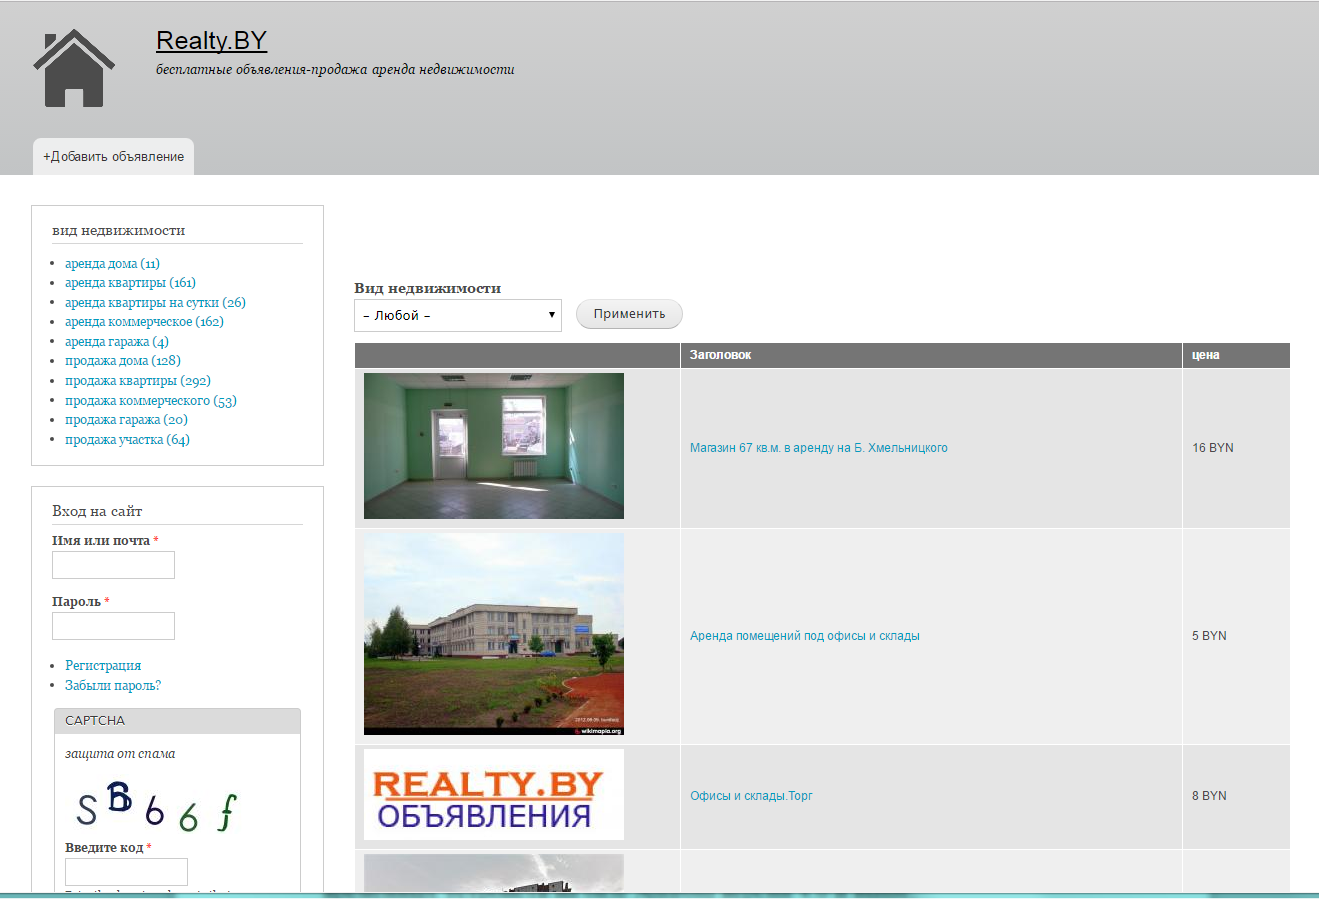
\includegraphics[scale=0.25]{realt1.png}
	\caption{ Главный страница программного средсва }
	\label{fig:arch_and_mod::realt1}
	\clearpage
\end{figure}

Реалт.бай это простой способ для размещения объявлений в сети. Веб-интерфейс простой в использовании, все объявления хранятся в базе данных.

Реалт.бай это портал, на котором собрана вся информация о жилой и коммерческой недвижимости в Беларуси. На сайте можно найти информа-цию по вопросам аренды квартир и комнат в Минске, продаже квартир.

Прежде чем добавить объявление, необходимо пройти процедуру регистрации на сайте. Операция по добавлению нового объявления выглядит следующим образом. Пользователю необходимо добавить описание, тему заголовка, цену,  добавить контактные данные. После этого будет размещено объявление.

\begin{figure}[!htb]
	\centering
	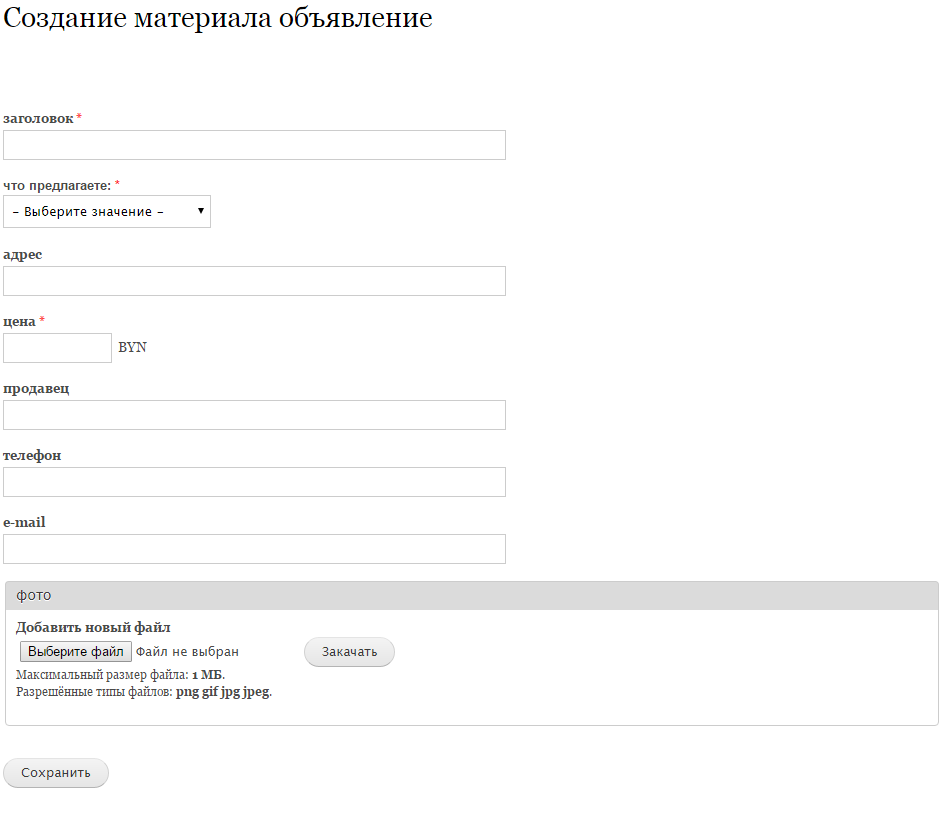
\includegraphics[scale=0.3]{realt2.png}
	\caption{ Добавление нового объявления }
	\label{fig:arch_and_mod::realt2}
	\clearpage
\end{figure}

Среди возможностей программного средства реалт.бай  можно выде-лить следующие достоинства:

\begin{itemize}
	\item понятный и простой интерфейс.
	\item возможность размещать объявление не только о продажи недвижимости.
	\item легкая обратная связь между клиентом и риелтором.
\end{itemize}

Помимо всех плюсов, стоит отметить несколько минусов данного программного средства:

\begin{itemize}
	\item только один критерий для поиска объявлений.
	\item нет возможности редактирования информации.
	\item большинство предложений уже не актуально.
\end{itemize}

Таким образом, это программное средство подходит в качестве простого приложения, решающее только частично описанные проблемы.

\subsubsection{Программное средство квартирант.бай}

Квартирант.бай это программное средство, предоставляющее следующий перечень услуг:

\begin{itemize}
	\item аренда квартир;
	\item аренда комнат;
	\item аренда гостинец;
	\item продажа недвижимости;
\end{itemize}

\begin{figure}[!htb]
	\centering
	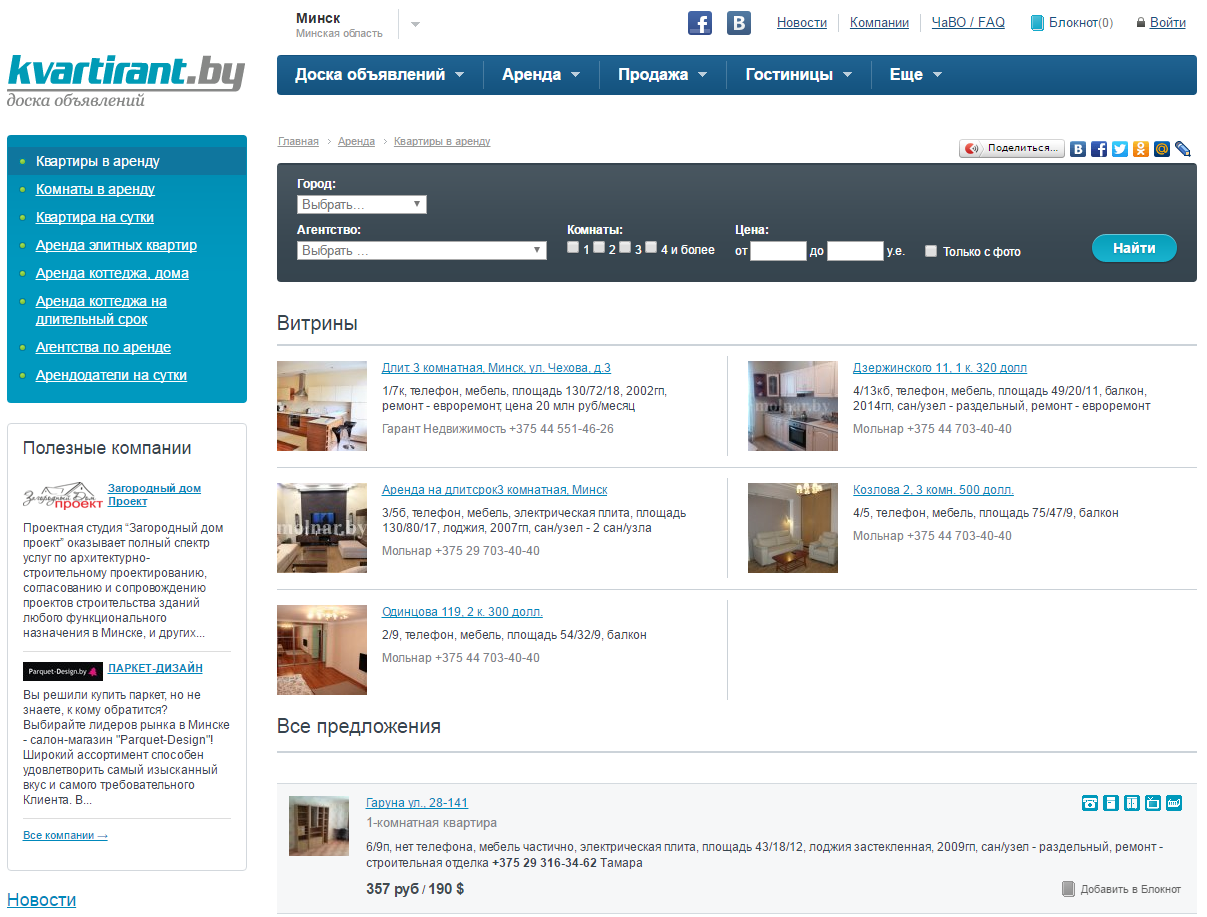
\includegraphics[scale=0.3]{kv_1.png}
	\caption{ Доска объявлений }
	\label{fig:arch_and_mod::lexer_flow}
	\clearpage
\end{figure}

Проект квартирант.бай стартовал в 2004 году как специализированный сайт по аренде всех видов недвижимости. Доска объявлений портала Квартирант.бай является популярной площадкой для бронирования гостинец, покупки недвижимости, аренды квартир.

Среди возможностей программного средства y можно выделить следующие достоинства:

\begin{itemize}
	\item понятный интерфейс;
	\item легкая обратная связь между клиентом и риелтором;
	\item возможность размещать объявление не только о продажи недвижимости;
\end{itemize}

Помимо всех плюсов, стоит отметить несколько минусов данного программного средства:

\begin{itemize}
	\item реклама;
	\item нет возможности редактирования информации;
	\item нет возможности оставить отзывы;
\end{itemize}

Таким образом, это программное средство подходит в качестве приложения, решающе не все описанные проблемы.

% \begin{explanation}

\subsubsection{Программное средство сильван}

Программное средство оказывает услуги в сфере недвижимости. Продажа, покупка, обмен, разъезд, аренда комнат, квартир, коттеджей, дач, земельных участков, коммерческой недвижимости. Приватизация, утверждение перепланировок, вывод в нежилой фонд, консервация и другое.

\begin{figure}[!htb]
	\centering
	
\includegraphics[scale=0.3]{sl_1.png}
	\caption{ Главная форма программного средства}
	\label{fig:arch_and_mod::lexer_flow}
	\clearpage
\end{figure}

Среди возможностей программного средства y можно выделить следующие достоинства:

\begin{itemize}
	\item обратная связь между клиентом и риелтором;
	\item возможность поиска по различным критериям;
\end{itemize}

Стоит отметить минусы данного программного средства:

\begin{itemize}
	\item яркий дизайн;
	\item нет пользователей как таковых
	\item нет возможности редактирования информации;
	\item нет возможности оставить отзывы;
	\item нет возможности добавить объявление;
	\item все операции делаются в ручную, клиент должен обратиться в офис компании;
\end{itemize}

Таким образом, данное программное средство не решает  множество описанных проблемы. Программное средство представляет из себя частный случай для риэлтерской компании.

\subsection{Постановка задачи}
В результате выполнения дипломного проекта должно быть разработано программное средство для продажи квартир через веб-интерфейс. 

Необходимо выполнить следующие задачи:

\begin{itemize}
	\item изучить и улучшить знания в web разработке приложения;
	\item ознакомиться с многопоточными приложениями и особенностями платформы java;
	\item разработать программное средство для продажи квартир; 
	\item разработать масштабируемое приложение, чтобы была возможность в будущем реализовывать дополнительный функционал;
\end{itemize}

Программное средство должно иметь два уровня доступа: администратор и пользователь. Пользователь может иметь доступ к своей учетной записи для добавления, поиска, редактирования своих объявлений. Администратор должен иметь возможность настраивать веб-интерфейс и управлять зарегистрированными пользователями.

Должны быть реализованы следующие ключевые функции:

\begin{itemize}
	\item создание учетной записи пользователя;
	\item восстановление учетной записи пользователя;
	\item добавление объявления;
	\item редактирование объявления;
	\item удаления  объявления;
	\item добавление фотографий;
	\item поиск объявления по множеству критериев;
	\item возможность оставить отзыв;
\end{itemize}

В процессе дипломного проектирования необходимо разработать приложение, которое будет решать все поставленные задачи и основные функции.


\lstset{style=fsharpstyle}

\section{Анализ требований к программному средству}

\subsection{Используемые технологии}
\label{sec:practice:technology_used}

Выбор технологий является важным предварительным этапом разработки сложных информационных систем.
Платформа и язык программирования, на котором будет реализована система, заслуживает большого внимания, так как исследования показали, что выбор языка программирования влияет на производительность труда программистов и качество создаваемого ими кода.

Ниже перечислены некоторые факторы, повлиявшие на выбор технологий:
\begin{itemize}
\item разрабатываемое ПО должно иметь возможность запускаться под платформами Windows(7,8,10) и Linux(Ubuntu, Arch Linux, Linux Mint);
\item ПО работает в совокупности с другими средствами описания аппарутры интегральных схем и должно иметь возможность запускаться в форме скрипта;
\item среди различных платформ разработки имеющийся программист лучше всего знаком с разработкой на платформе;
\item дальнейшей поддержкой проекта, возможно, будут заниматься разработчики, не принимавшие участие в выпуске первой версии;
\item имеющийся разработчик имеет опыт работы с объекто-ориентированными языками программирования;
\end{itemize}

Основываясь на опыте работы имеющихся программистов разрабатывать ПО целесообразно с помощью языка Java.
Приняв во внимание необходимость обеспечения доступности дальнейшей поддержки ПО, возможно, другой командой программистов, необходимость работы с различными ОС, скриптообразный характер ПО, целесообразно не использовать малоизвестные и сложные языки программирования.

С учетом этого фактора выбор языков программирования сужается до четырех: Python, Ruby и Java. Слабые по сравнению с другими языками механизмы ООП (отсутствие наследования, классов) языка LUA, которые могут быть полезны при разработке ПО, позволяют исключить этот язык из списка кандидатов. Python уступает по удобству использования двум другим кандидатам из нашего списка. Оставшиеся два языка программирования Ruby и Java являются хорошими кандидатами . Тот факт, что Java существует на рынке уже давно, делает этот язык предпочтительным кандидатом.

Таким образом, с учетом вышеперечисленных факторов, целесообразно остановить выбор на следующих технологиях:
\begin{itemize}
  \item операционные системы: семейство Windows(7,8,10), семейство Linux(Ubuntu, Debian, Arch Linux), Mac os;
  \item база данных MySql для хранения информации;
  \item язык программирования Java на котором будет реализована серверная часть программного средства;
  \item язык программирования Javascript и библиотека react js;
\end{itemize}
При реализации программного средства встает вопрос, в каком виде должна храниться вся информация и с помощью каких средств её следует обрабатывать. Так как, например, информация о каждом отдельном объявлении представляет собой типичный набор данных (площадь, количество комнат, этаж, год постройки и т. д.), то очевидно, что в этом случае целесообразно хранить их в реляционной базе данных на сервере. Посредством запросов к базе данных пользователь может получать нужные ему сведения, а администратор может добавлять и изменять данные. Выбор конкретной СУБД в качестве сервера баз данных осуществлялся исходя из тех преимуществ, которые она имеет перед другими, а также удобства работы с ней. В данном случае был выбрана клиент-серверная СУБД MySQL

Для реализации поставленной задачи предпочительно использовать на ранних этапах базу данных MySql. В случаи большого количество информации, можно будет слегкость мигрировать на другую СУБД, т.к язык Java использует спецификацию JPA, которая позволяет с легкостью мигрировать на другую СУБД.

Объектно-ориентированный язык программирования Java широко используется для создания серверных приложений. Язык java будет использован для создания высокоуровнего дизайна проложения (иерархия классов и интерфейсов, организация модулей и публичного программного интерфейса), реализации логики приложения, функций и методов~\cite{dpir_2007}, прототипирования различных идей.

Для реализации клиентской части был выбран язык программирования Javascript. Для быстроты и удобства реализации, будет использована библиотека react.js, которая написана на языке программирования Javascript. 


\subsubsection{Язык программирования Java}
\label{sub:practice:ruby_overview}
Объектно-ориентированный язык программирования Java широко используется для создания серверных приложений.

Система Java создана на основе простого языка программирования, техника использования которого близка к общепринятой и обучение которому не требует значительных усилий.

Java как язык программирования является объектно-ориентированным с момента основания. Кроме того программист с самого начала обеспечивается набором стандартных библиотек, обеспечивающих функциональность от стандартного ввода/вывода и сетевых протоколов до графических пользовательских интерфейсов. Эти библиотеки легко могут быть расширены.

Несмотря на то, что язык С++ был отвергнут, синтаксис языка Java максимально приближен к синтаксису С++. Это делает язык знакомым широкому кругу программистов. В то же время из языка были удалены многие свойства, которые делают С++ излишне сложным для пользования, не являясь абсолютно необходимыми. В результате язык Java получился более простым и органичным, чем С++.

Надежность и безопасность Java существенно облегчает создание надежного программного обеспечения. Кроме исчерпывающей проверки на этапе компиляции, система предусматривается анализ на этапе выполнения. Сам язык спроектирован так, чтобы вырабатывать у программиста привычку писать "правильно". Модель работы с памятью, в которой исключено использование указателей, делает невозможными целый класс ошибок, характерных для С и С++.

В силу того, что Java предназначен для работы в распределенной среде, безопасность становится чрезвычайно важной проблемой. Требования безопасности определяют многие черты как языка, так и реализации всей системы.
Компилятор Java производит байт-коды, т.е. модули приложения имеют архитектурно-независимый формат, который может быть проинтерпретирован на множестве разнообразных платформ. Это уже не исходные тексты, но еще не платформно-зависимые машинные коды.

Схема работы системы и набор байт-кодов виртуальной машины Java таковы, что позволяют достичь высокой производительности на этапе выполнения программы:

анализ кодов на соблюдение правил безопасности производится один раз до запуска кодов на выполнение, в момент выполнения таких проверок уже не нужно, и коды выполняются максимально эффективно ;

работа с базовыми типами максимально эффективна, для операций с ними зарезервированы специальные байт-коды;

методы в классах не обязательно связываются динамически;

автоматический сборщик мусора работает отдельным фоновым потоком, не замедляя основную работу программы, но в то же время обеспечивая своевременный возврат свободной памяти в систему;

стандарт предусматривает возможность написания критических по производительности участков программы в машинных кодах;

Каждая из перечисленных характеристик по отдельности может быть найдена в уже существующих программных пакетах. Новым является соединение их в стройную непротиворечивую систему, которая должна стать всеобщим стандартом.

Java полагается на автоматическое управление памятью со стороны исполняющей среды, предоставляя совсем немного средств для управления жизненным циклом объектов.
Не смотря на это, в языке все же присутствуют указатели на функции.

Создатели языка Java не являются противниками привнесения в язык новых идей и возможностей.
Каждая новая версия интерпретатора языка привносит различные полезные возможности, которые отвечают требованиям индустрии.


\subsubsection{Система управления базами данных MySQL}
\label{sub:practice:vhdl_overview}
Выбор конкретной СУБД в качестве сервера баз данных осуществлялся исходя из тех преимуществ, которые она имеет перед другими, а также удобства работы с ней. В данном случае был выбрана клиент-серверная СУБД MySQL. Её архитектура изображена на рисунке ниже. 

\begin{figure}[!htb]
	\centering
	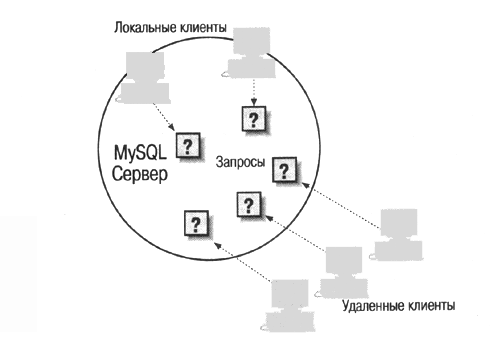
\includegraphics[scale=0.5]{mysql.png}
	\caption{ Клиент-серверная архитектура MySQL}
	\label{fig:arch_and_mod::lexer_flow}
	\clearpage
\end{figure}

Клиент-серверная архитектура MySQL
Самая подходящая для MySQL сфера применения - это Интернет, благодаря хорошей системе безопасности этого пакета, стабильной работе и высокому быстродействию. Для создания скриптов был выбран язык программирования PHP, а MySQL – самая популярная СУБД, которая поддерживается этим языком. В PHP есть множество функций, которые позволяют удобно и эффективно работать с базами данных – и это одна из причин выбора данной СУБД.

Рассмотрим преимущества MySQL:

\begin{itemize}

	\item Быстродействие. Благодаря внутреннему механизму многопоточности быстродействие MySQL весьма высоко. Для разработчиков MySQL скорость всегда являлась ключевым параметром. Новые возможности добавлялись в пакет MySQL только после того, как их удавалось реализовать без ущерба для производительности. Иногда это означало, что некоторые возможности добавлялись не так быстро, как хотелось бы пользователям, но зато всегда гарантировало быструю работу MySQL.

	\item Безопасность. Довольно высокий уровень безопасности обеспечивается благодаря базе данных mysql, создающейся при установке пакета и содержащей пять таблиц. При помощи этих таблиц можно описать, какой пользователь из какого домена с какой таблицей может работать и какие команды он может применять. Пароли, хранящиеся в базе данных, можно зашифровать при помощи встроенной в MySQL функции password().

	\item Лицензия.Раньше лицензирование MySQL было немного запутанным; сейчас эта программа для некоммерческих целей распространяется бесплатно.

	\item Открытость кода. Благодаря этому программист может сам добавлять в пакет нужные функции, расширяя его функциональность так, как ему требуется. За отдельную плату это могут сделать и сами авторы MySQL. 

	\item Простота использования. Для начала работы с MySQL не требуется сложной процедуры конфигурации. MySQL Server начнёт работать соответствующим образом сразу. По умолчанию выбираются значения, соответствующие минимальному использованию ресурсов диска и памяти. Для получения оптимальной производительности и для специальных условий (например, для проверки входа в систему), конечно же, потребуется дополнительная настройка. Чтобы помочь выполнить такую настройку, предлагаются соответствующие примеры файлов типовой конфигурации.

	\item Сообщество. Как следствие открытости кода, бесплатности программы, стабильной и надежной ее работы образовалось сообщество людей, которые не просто лояльны к MySQL, но и всячески участвуют как в развитии самого пакета, так и в обучении менее опытных людей работе с ним. Существует огромное количество листов рассылки и конференций, где можно получить бесплатную помощь в любое время суток.
\end{itemize}

В настоящее время существуют версии программы для большинства распространенных компьютерных платформ. Это говорит о том, что вам не навязывают определенную операционную систему. Вы сами можете выбрать, с чем работать, например с Linux или Windows, но даже в случае замены ОС вы не потеряете свои данные и вам даже не понадобятся дополнительные инструменты для их переноса.
Конечно же, как и любое программное средство, СУБД MySQL не избавлена от некоторых недостатков. Например, можно назвать отсутствие вложенных запросов, что приводит к необходимости находить нужные значения отдельно и подставлять их в другой запрос непосредственно в CGI-сценарии, что, несомненно, сказывается на производительности.
Несмотря на это, СУБД MySQL была выбрана как наиболее подходящий сервер баз данных для программного средства.

\subsubsection{Язык программирования Javascript}

JavaScript — прототипно-ориентированный сценарный язык программирования. Является реализацией языка ECMAScript (стандарт ECMA-262).

JavaScript обычно используется как встраиваемый язык для программного доступа к объектам приложений. Наиболее широкое применение находит в браузерах как язык сценариев для придания интерактивности веб-страницам.

Основные архитектурные черты: динамическая типизация, слабая типизация, автоматическое управление памятью, прототипное программирование, функции как объекты первого класса.

Структурно JavaScript можно представить в виде объединения трёх чётко различимых друг от друга частей:

\begin{itemize}
	\item ядро (ECMAScript),
	\item объектная модель браузера (Browser Object Model или BOM (en)),
	\item объектная модель документа (Document Object Model или DOM).
\end{itemize}

Если рассматривать JavaScript в отличных от браузера окружениях, то объектная модель браузера и объектная модель документа могут не поддерживаться.

Объектную модель документа иногда рассматривают как отдельную от JavaScript сущность, что согласуется с определением DOM как независимого от языка интерфейса документа. В противоположность этому ряд авторов находят BOM и DOM тесно взаимосвязанными.

На JavaScript оказали влияние многие языки, при разработке была цель сделать язык похожим на Java, но при этом лёгким для использования непрограммистами. Языком JavaScript не владеет какая-либо компания или организация, что отличает его от ряда языков программирования, используемых в веб-разработке.

JavaScript является объектно-ориентированным языком, но используемое в языке прототипирование обуславливает отличия в работе с объектами по сравнению с традиционными класс-ориентированными языками. Кроме того, JavaScript имеет ряд свойств, присущих функциональным языкам — функции как объекты первого класса, объекты как списки, карринг, анонимные функции, замыкания — что придаёт языку дополнительную гибкость.

Несмотря на схожий с Си синтаксис, JavaScript по сравнению с языком Си имеет коренные отличия:

\begin{itemize}
	\item объекты, с возможностью интроспекции;
	\item функции как объекты первого класса;
	\item автоматическое приведение типов;
	\item автоматическая сборка мусора;
	\item анонимные функции;
\end{itemize}

В языке отсутствуют такие полезные вещи, как:

\begin{itemize}
	\item JavaScript не предоставляет возможности управлять зависимостями и изоляцией областей видимости;
	\item отсутствует интерфейс программирования приложений по работе с файловой системой, управлению потоками ввода-вывода, базовых типов для бинарных данных;
	\item стандартные интерфейсы к веб-серверам и базам данных;
	\item система управления пакетами которая бы отслеживала зависимости и автоматически устанавливала их;
\end{itemize}

React является библиотекой, написаной на JavaScript с открытым исходным кодом для создания пользовательских интерфейсов. Библиотека была написана разработчиками из Facebook, Instagram и сообществом индивидуальных разработчиков и корпораций. 

React позволяет разработчикам создавать крупные веб-приложения, которые используют данные, которые могут меняться со временем, без перезагрузки страницы. Его основная цель - быть быстрым, простым и масштабируемым. 

Клиентская часть программного средства, будет разработана с помощью языка Javascript и библиотеки Ract.

\subsection{Функциональное моделирование}

Для функционального моделирования программного средства для продажи квартир использована диаграмма вариантов использования, являющаяся частью унифицированного языка моделирования (UML).
Общий вид обобщенной диаграммы вариантов использования удаленного управления мультимедиа представлен ниже.

\begin{figure}[!htb]
	\centering
	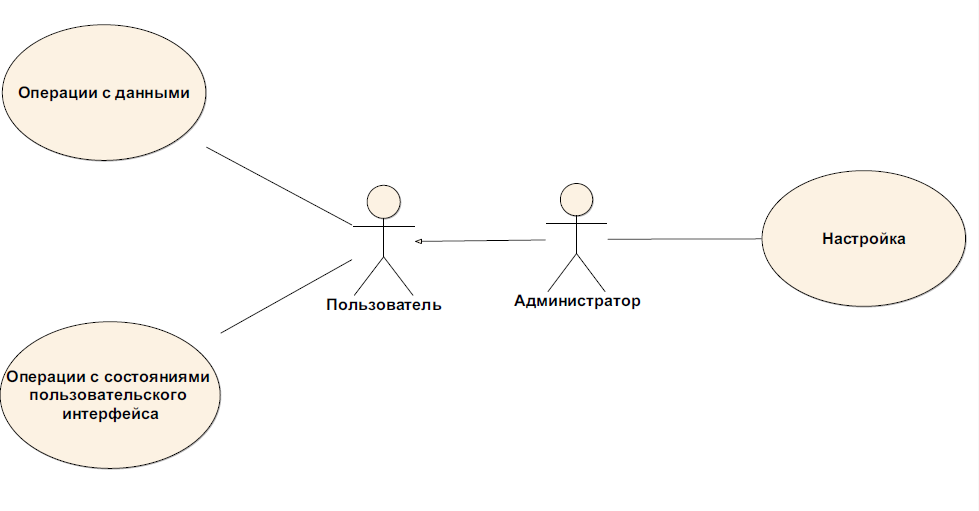
\includegraphics[scale=0.5]{general_use_case.png}
	\caption{ Диаграмма вариантов использования}
	\label{fig:arch_and_mod::lexer_flow}
	\clearpage
\end{figure}

Как видно из диаграммы, для программного средства необходимы два актера:

\begin{itemize}
	\item пользователь – это любой конечный пользователь из круга лиц, имеющий доступ к удаленному управлению данными на устройствах;
	\item администратор – это такой пользователь, который кроме всех обычных функций, доступных пользователю, имеет еще специфические функции настройки данных; следует отметить, что администратор наследуются от пользователя.
\end{itemize}

Среди основных функций пользователя можно выделить:

\begin{itemize}
	\item операции с данными: все функции, связанные с отображением и управлением мультимедийных данных, дополнительные специфические функции с мультимедиа;
	\item операции с состояниями пользовательского интерфейса: все функ-ции, предназначенные для управления состояниями пользовательского ин-терфейса.
\end{itemize}

У администратора следует выделить функции настройки программного средства, предназначенные настройки всех компонент, связанных с коректной работой пользователя.

Рассмотрим необходимые функции для работы с объявлениями. диаграмма вариантов использования «Работа с объявлениями» представлена ниже.

\begin{figure}[!htb]
	\centering
	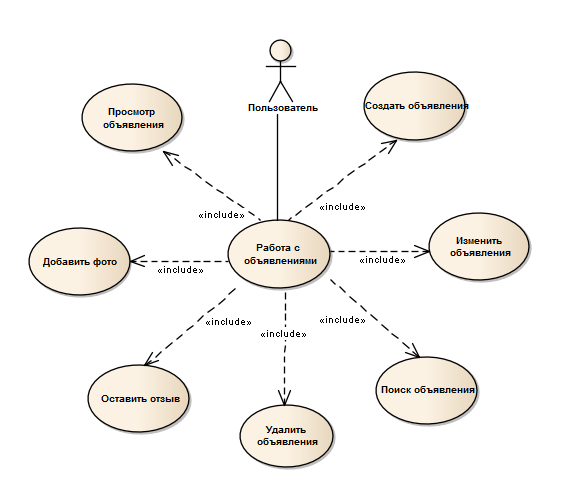
\includegraphics[scale=0.8]{notes_use_case.png}
	\caption{ диаграмма вариантов использования «Работа с объявлениями»}
	\label{fig:arch_and_mod::lexer_flow}
	\clearpage
\end{figure}

Как видно из диаграммы, функция «Работа с объявлениями» включает в себя следующие возможности:

\begin{itemize}
	\item «Создать объявления»: данная функция дает возможность пользователю создавать объявления для возможности выставить свою недвижимость на продажу. 
	\item «Изменить объявление»: функция означает возможность пользователем изменять ранее созданные объявления. Включает возможность редактирования информация, которая была описана при создании объявления.
	\item «Поиск объявления»: такая функция означает возможность пользователя поиска объявления для покупки или аренды недвижимости. Данная функция включает в себя множество критериев для поиска.
	\item «Удалить объявления»: функция означает возможность удалить выбранное объявление.
	\item «Оставить отзыв»: функция дает возможность пользователем добавлять комментарии, задавать дополнительные вопросы на счет недвижимости.
	\item «Добавить фото»: функция означает возможность пользователю добавить фото о недвижимости.
	\item «Просмотр объявления»: функция дает возможность пользователям просматривать объявление о недвижимости.
\end{itemize}

Рассмотрим подробнее функцию «Создать новое объявление». Диаграмма вариантов использования представлена ниже.


\begin{figure}[!htb]
	\centering
	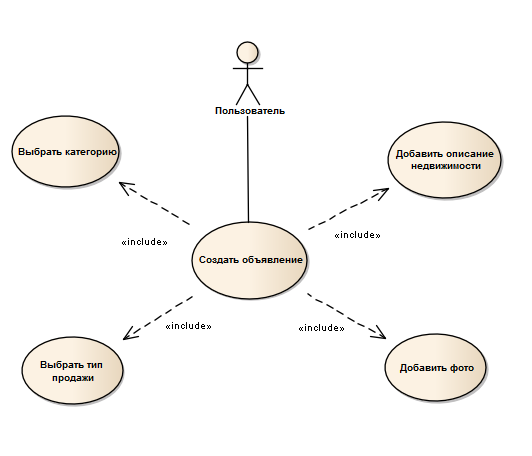
\includegraphics[scale=0.8]{create_note_use_case.png}
	\caption{ Диаграмма вариантов использования «Создать объявление»}
	\label{fig:arch_and_mod::lexer_flow}
	\clearpage
\end{figure}

Как видно из диаграммы, функция «Создать объявления» включает в себя следующие возможности:

\begin{itemize}
	\item «Добавить описание недвижимости»: данная функция дает возможность пользователю добавить необходимую информацию о своей недвижимости. Данная информация будет видна другим пользователям.  
	\item «Добавить фото»: функция означает возможность пользователю добавить фотографии о недвижимости. Например пользователь может добавить фотографию планировки квартиры, фотографию гостиной, фотографию кухни и т.д .
	\item «Выбрать тип продажи»: эта функция дает возможность пользователя выбрать тип продажи недвижимости. Будет это аренда жилья, чистая продажа недвижимости или обмен с доплатой.
	\item «Выбрать категорию»: эта функция дает возможность пользователя выбрать категорию объявления. В зависимости от категории, будущее объявление будет размещено в нужной секции. Это функция облегчает поиск для других клиентов.
\end{itemize}

Рассмотрим необходимые функции для роли «Администратор». Диаграмма вариантов использования представлена ниже.

\begin{figure}[!htb]
	\centering
	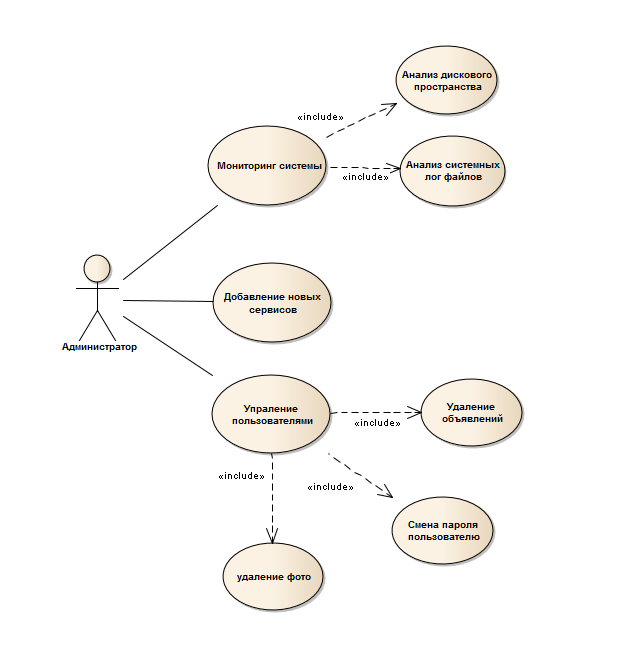
\includegraphics[scale=0.8]{admin_use_case.png}
	\caption{ Диаграмма вариантов использования для роли «Администратор»}
	\label{fig:arch_and_mod::lexer_flow}
	\clearpage
\end{figure}

Данная диаграмма показывает, какими функциями должен обладать пользователь, с ролью администратор.  Рассмотрим каждую функции в подробном описании:

\begin{itemize}
	\item «Анализ дискового пространства»: данная функция дает возможность администратору смотреть свободное место дискового пространства. Данная функция необходима, чтобы периодически чистить устаревшую информацию, которая будет храниться на диске.
	\item «Анализ системных лог файлов»: функция означает возможность администратору просматривать системные лог файлы на наличие ошибок. В случаи сбоя приложения, пользователю необходима узнать по какой причине произошёл сбой. 
	\item «Добавление новых сервисов»: эта функция дает возможность администратору добавить новый сервис. данная функция предназначена для расширения функционала будущего программного средства. 
	\item «Удаление объявления»: эта функция дает возможность администратору удалить любое объявление. Данная функция предназначена для удаления устаревших и неактуальных объявлений, в случаи, если пользователь сам не удалил объявление.
	\item «Удаление фото»: эта функция дает возможность администратору удалить любые фотграфии. Данная функция предназначена для удаления устаревших и неактуальных фотографий в случаи, если пользователь сам не удалил объявление.
	\item «Смена пароля пользователю»: функция дает возможность администратору сменить пароль пользователю. Например, если пользователь не смог восстановить пароль с помощью стандартных методов, он может обратиться в сервисный центр.
\end{itemize}

Для возможности пользоваться программным средством, необходима учётная запись.  

Учётная запись это хранимая в компьютерной системе совокупность данных о пользователе, необходимая для его опознавания (аутентификации) и предоставления доступа к его личным данным и настройкам. Учётная запись, как правило, содержит сведения, необходимые для опознания пользователя при подключении к системе, сведения для авторизации и учёта. Это идентификатор пользователя (login) и его пароль. Пароль, как правило, хранится в зашифрованном или хэшированном виде для обеспечения его безопасности. Для использования учётной записи (другими словами, для входа в систему под чьим-то именем) необходимо использовать логин и пароля. Для регистрации необходимо использовать дополнительное поле email. 

Рассмотрим необходимые функции для работы с учетной записью. Данная диаграмма показывает, что пользователь может делать с учетной записью. 

Диаграмма вариантов использования представлена ниже.

\begin{figure}[!htb]
	\centering
	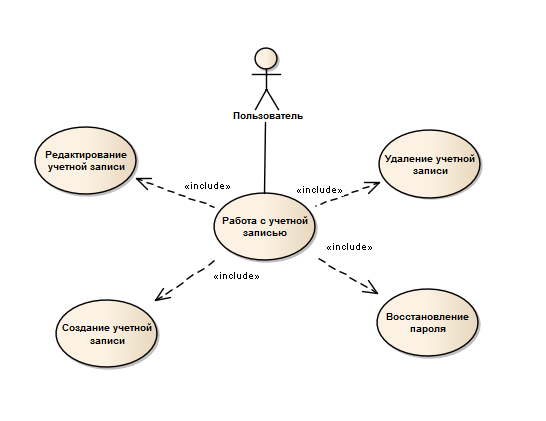
\includegraphics[scale=0.8]{account_use_case.png}
	\caption{ Диаграмма вариантов использования «Работа с учетной записью»}
	\label{fig:arch_and_mod::lexer_flow}
	\clearpage
\end{figure}

Рассмотрим каждую функцию подробнее:

\begin{itemize}
	\item «Создание учетной записи»: данная функция дает возможность пользователю завести учетную запись, чтобы использовать возможности программного средства.
	\item «Редактирование учетной записи»: данная функция позволяет пользователю изменить или дополнить информацией свою учетную запись.
	\item «Удаление учетной записи»: данная функция позволяет пользователю удалить свою учетную запись.
	\item «Восстановление пароля»: данная функция дает возможность пользователю востановить пароль от учетной записи. 
\end{itemize}

\subsection{Разработка спецификации функциональных требований}

На основе функциональной модели ПС и поставленных задач необходимо разработать спецификацию функциональных требований к программному средству для продажи квартир.

Спецификация функционального требования «Создание учетной записи пользователя»:

\begin{itemize}
	\item Функции создания учетной записи должна быть доступна только клиентам;
	\item При нажатии пользователем на кнопку «sign up» на экране отображается окно, в котором пользователь должен указать логин, пароль, электронную почту;
	\item  После нажатия на кнопку “create” в системе должен появиться новый пользователь. Должно произойти перенаправление на страницу входа в программное средство; 
	\item Если логин или электронная почта уже используется у другого пользователя, ПС должно предложить пользователю ввести другой логин и электронную почту, т.к такие данные уже используются;
\end{itemize}

Спецификация функционального требования «Восстановление учетной записи пользователя»:

\begin{itemize}
	\item Функции должна быть доступна только клиентам;
	\item При нажатии пользователем на кнопку «forgot password» на экране отображается окно, в котором пользователь должен указать свою  электронную почту для восстановления пароля;
	\item После нажатия на кнопку “restore” на почту должны прийти инструкции как восстановить пароль. Должно произойти перенаправление на страницу входа в программное средство; 
\end{itemize}


Спецификация функционального требования «Добавление объявления»:

\begin{itemize}
	\item Функции должна быть доступна только клиентам;
	\item При нажатии пользователем на кнопку «forgot password» на экране отображается окно, в котором пользователь должен указать свою  электронную почту для восстановления пароля;
	\item  После нажатия на кнопку “restore” на почту должны прийти инструкции как восстановить пароль. Должно произойти перенаправление на страницу входа в программное средство;
\end{itemize}

Спецификация функционального требования «редактирование объявления»:

\begin{itemize}
	\item Функции должна быть доступна только клиентам;
	\item Функция редактирования мультимедиа должна быть доступна, после выбора файла и отмечена галочкой;
	\item Нажатие пользователем во время редактирования клавиши «Cancel» должно отменить редактирование;
	\item При нажатии пользователем во время редактирования на клавишу «Enter» редактируемое мультимедиа должно быть сохранено;
	\item После редактирования выбранного мультимедиа страница должна быть обновлена;
\end{itemize}

Спецификация функционального требования «удаления  объявления»:

\begin{itemize}
	\item Функции должна быть доступна всем;
	\item При нажатии пользователем на кнопку удаления должно быть показано окно с подтверждением удаления; 
	\item После удаления выбранного мультимедиа страница должна быть обновлена;
\end{itemize}

Спецификация функционального требования «добавление фотографий»:

\begin{itemize}
	\item Функции должна быть доступна только клиентам;
	\item на странице объявления должна присутствовать кнопка «Add photo». При нажатии на кнопку,  появляется диалоговое окно;
	\item в диалоговом окне должны быть кнопки «choose photo», «add», «cancel»;
	\item при нажатии кнопки «choose photo» пользователь должен выбрать фото;
	\item после нажатия кнопки «Add» выбранная фотография появляется на странице объявления;
	\item при нажатии кнопки «cancel» происходит отмена данной операции;
\end{itemize}

Спецификация функционального требования «поиск объявления»:

\begin{itemize}
	\item Функции должна быть доступна только клиентам;
	\item На главной странице должна присутствовать панель для поиска объявлений;
	\item На панели должны быть следующие критерии для поиска: ценовой диапазон, город, район, количество комнат, типа продажи, тип категории, кнопка «Search»;
	\item При нажатии на кнопку «Search» в центре экрана появляются найденные объявления;
\end{itemize}

Спецификация функционального требования «Добавления отзывы»:

\begin{itemize}
	\item Функции должна быть доступна только клиентам;
	\item на странице объявления должна присутствовать кнопка «Add comment». При нажатии на кнопку, появляется диалоговое окно;
	\item после нажатия кнопки «Add» отзыв появляется на странице объявления;
\end{itemize}




\section{Архитектура и модули системы} % (fold)
\label{sec:arch_and_mod}

Разработанное программное средство представляет из себя клиент-серверное приложение, в котором клиентом выступает браузер, а сервером — веб-сервер. Логика веб-приложения распределена между сервером и клиентом, хранение данных осуществляется, преимущественно, на сервере, обмен информацией происходит по сети. Одним из преимуществ такого подхода является тот факт, что клиенты не зависят от конкретной операционной системы пользователя. Исходя из выше сказанного, можно сказать, что веб-приложения являются кроссплатформенными сервисами. Серверная часть приложения реализована с помощью языка Java. Клиентская часть реализована с помощью языка Javascript [6].

Серверная часть состоит из следующих модулей:
\begin{itemize}
	\item модуль доступа к данным (DAO);
	\item модуль сервисов(Бизнес логика);
	\item модуль предоставления данных(Форматирование данных);
\end{itemize}

Клиентская часть состоит из следующих компонентов:
\begin{itemize}
	\item модуль действий(actions);
	\item модуль отображений(components);
\end{itemize}

Рассмотрим каждый компонент по отдельности. 

\subsection{Модуль доступа к данным}
\label{sub:arch_and_mod:lexer}

Данный модуль дает возможность доступа к базе данных. Для реализации данной функциональности использовался шаблон проектирования DAO. 

Шаблон проектирования DAO -- это объект, который предоставляет абстрактный интерфейс к какому-либо типу базы данных или механизму хранения. Определённые возможности предоставляются независимо от того, какой механизм хранения используется и без необходимости специальным образом соответствовать этому механизму хранения. Этот шаблон проектирования применим ко множеству языков программирования, большинству программного обеспечения, нуждающемуся в хранении информации и к большей части баз данных. На данном  уровне нет механизма для управления транзакциями, т.к. транзакции как правило принимают участие в бизнес операциях [7].  

В качестве выбора данного шаблона, послужили следующие факторы:

\begin{itemize}
	\item DAO инкапсулирует доступ к источнику данных;
	\item DAO является реализацией слоя объектно-реляционного отображения;
	\item DAO более ориентирован на источник данных;
\end{itemize}


Основная цель данного модуля --- упростить процесс взаимодействия с БД. Пример реализации шаблона DAO приведены в листинге~\ref{lst:arch_and_mod:DAO}:

\begin{lstlisting}[language=Java, style=rubystyle, caption={Определение для доступа к данным}, label=lst:arch_and_mod:DAO]
public interface IDAO<Key extends Serializable, E> {

E create(E entity);

E read(Key key);

void update(E entity);

void delete(E entity);

}

public abstract class AbstractDAOImp<Key extends Serializable, E> implements IDAO<Key, E> {

@Autowired
private SessionFactory sessionFactory;

private Class<E> clazz;

protected AbstractDAOImp(Class<E> clazz) {
	this.clazz = clazz;
}

protected Session getSession() {
	return sessionFactory.getCurrentSession();
}

@Override
public E create(E entity) {
	Session session = getSession();
	session.persist(entity);
	session.flush();
	return entity;
}

@Override
public E read(Key key) {
	return getSession().find(clazz, key);
}

@Override
public void update(E entity) {
	getSession().update(entity);
}

@Override
public void delete(E entity) {
	getSession().delete(entity);
}

}

@Repository("UserRepository")
public class UserDAOImp extends AbstractDAOImp<Integer, User> {

protected UserDAOImp() {
	super(User.class);
}

public List<User> readAllUser() {
	return getSession().createQuery("from users", User.class).list();
}

}
\end{lstlisting}


\subsection{Модуль сервисов}~
\label{sec:arch_and_mod:regex}
На этом уровне реализована бизнес логика приложения, управление транзакциями, сервис для загрузки изображений и другие. 

Для начала рассмотрим сервис, который взаимодействует с модулем DAO. Сервис для взаимодейсвтия с DAO приведен в листинге~\ref{lst:arch_and_mod:Service1}:

\begin{lstlisting}[language=Java, style=rubystyle, caption={Использование DAO в сервисах}, label=lst:arch_and_mod:Service1]

@Service("UserService")
@Transactional
public class UserService {

@Autowired
private UserDAOImp daoImp;

public User addUser(User user) {
	return daoImp.create(user);
}

public void updateUser(User user) {
	daoImp.update(user);
}

public void removeUser(User user) {
	daoImp.delete(user);
}

public List<User> findAllUser() {
	return daoImp.readAllUser();
}

public User findUserById(int id) {
	return daoImp.read(id);
}

}

@Service("CommentService")
@Transactional
public class CommentService {

@Autowired
private CommentDAOImp daoImp;

public Post addPost(Comment comment){
return daoImp.create(comment);
}

public Post findCommentById(int id){
return daoImp.read(id);
}

public void updateComment(Post post){
daoImp.update(post);
}

public void removeComment(Post post){
daoImp.delete(post);
}

}

\end{lstlisting}

Сначала может показаться, что модуль сервис повторяет методы класса DAO. Но эти методы не просто повторяют, они оборачивают методы DAO с использованием транзакций. Транзакция это группа последовательных операций с базой данных, которая представляет собой логическую единицу работы с данными. Транзакция может быть выполнена либо целиком и успешно, соблюдая целостность данных и независимо от параллельно идущих других транзакций, либо не выполнена вообще, и тогда она не должна произвести никакого эффекта. Можно заметить, что модуль сервисов зависит от модуля DAO.

Рассмотрим сервис для загрузки и сохранения изображений. При разработке приложений была обнаружена проблема с быстрой загрузкой графического контента. Если картинки довольно большие, то необходимо обеспечить эффективную работу с памятью для предотвращения злополучной ошибки OutOfMemoryError. Так же во время загрузки изображения было необходимо показывать маленькое изображение. Именно данная проблематика и подталкивает обратиться к библиотеке с открытым исходным кодом – Universal Image Loader, целью которой является универсализация решения вышеописанной задачи в виде гибкого и конфигурируемого инструмента.

На данный момент библиотеку можно использовать в тех случаях, когда нужно загрузить и отобразить (и можно еще закэшировать) картинку из интернета или из файловой системы. Классические примеры применения ImageLoader'а – это списки, таблицы, галереи, где необходимо отображать изображения из сети.

Среди возможностей ImageLoader'а можно выделить следующие до-стоинства:

\begin{itemize}
	\item асинхронная загрузка и отображение изображений из интернета или с SD-карты;
	\item возможность кэширования загруженных картинок в памяти и/или на файловой системе устройства;
	\item возможность отслеживания процесса загрузки посредством «слушателей»;
	\item эффективная работа с памятью при кэшировании картинок в памяти;
	\item широкие возможности настройки ImageLoader'а.
\end{itemize}

К глобальным настройкам ImageLoader'а можно отнести:

\begin{itemize}
	\item максимальный размер кэшируемых в памяти картинок;
	\item тайм-аут для установки соединения и загрузки картинки;
	\item максимальное количество потоков для загрузки изображений, работающих одновременно;
	\item приоритет потоков по загрузке и отображению картинок;
	\item программная реализация дискового кэша (можно выбрать одну из готовых реализаций или создать свою собственную);
	\item программная реализация кэша в памяти (можно выбрать одну из готовых реализаций или создать свою собственную);
	\item опции загрузки изображения по умолчанию.
\end{itemize}

Опции загрузки изображения (применяются к каждому отдельному вызову ImageLoader.displayImage(...)) предоставляют возможность указать:

\begin{itemize}	
	\item отображать ли картинку – заглушку в ImageView, пока реальная картинка грузится (если да, то нужно указать эту «заглушку»);
	\item отображать ли какую-либо картинку в ImageView, если URL кар-тинки был передан пустым (если да, то нужно указать эту картинку); 
	\item кэшировать ли загруженную картинку в памяти;
	\item кэшировать ли загруженную картинку на файловой системе;
	\item тип декодирования изображения (максимально быстрый или мак-симально экономный для памяти).
\end{itemize}


\begin{figure}[!htb]
			\centering
			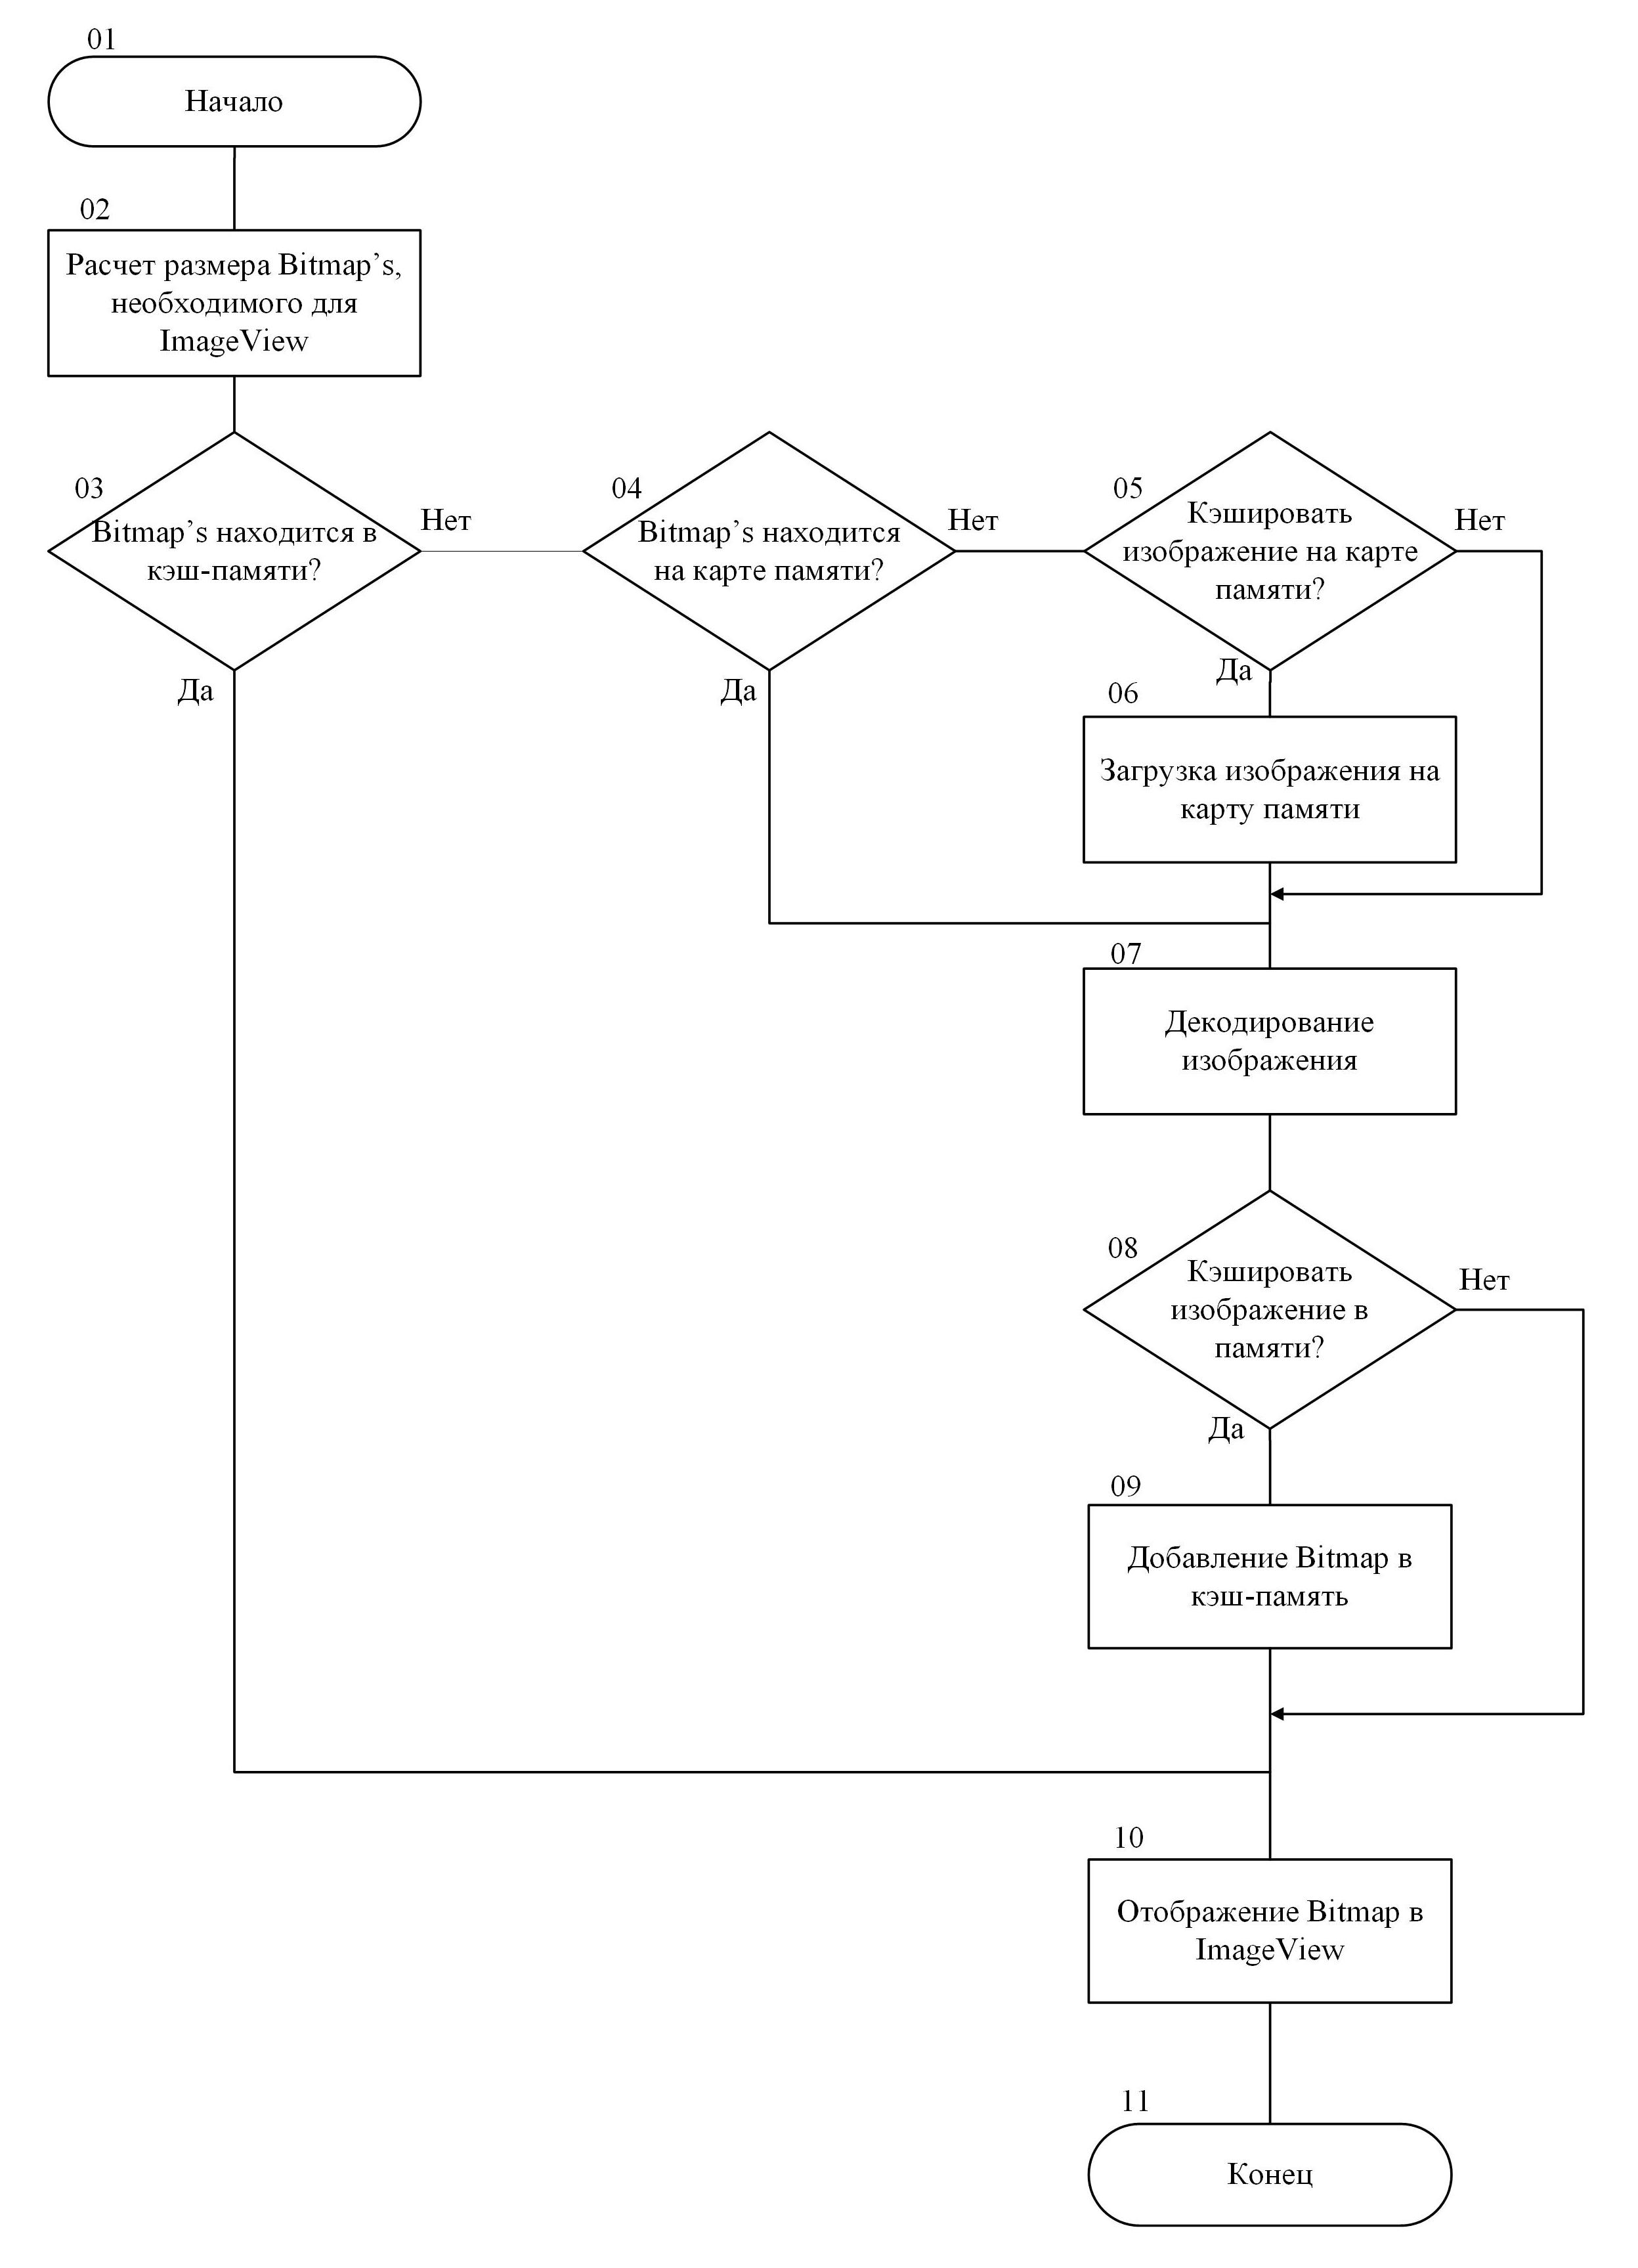
\includegraphics[scale=0.28]{loadImage.jpg}
			\caption{ Схема алгоритма ImageLoader }
			\label{fig:arch_and_mod:ImageLoader}
\end{figure}

Как уже упоминалось, программные реализации дискового кэша и кэша в памяти можно подключить свои. Но, скорее всего, будет достаточ-но готовых решений, которые в большинстве своем представляют собой кэши, ограниченные по какому-либо параметру (размер, количество файлов) и имеющие свою логику самоочищения при превышении лимита (FIFO, самый старый объект, самый большой объект, наиболее редко используемый) [8].


Каждая задача на загрузку и отображение картинки выполняется в отдельном потоке, кроме случаев, если картинка находится в кэше в памяти. Тогда она просто сразу отображается. Существует отдельная очередь потоков, куда попадают задачи, если нужная картинка закэширована на файловой системе. 

Если же нужной картинки нет в кэше, то задача-поток попадает в пул пото-ков. Таким образом, быстрому отображению закэшированных картинок ничего не препятствует.

Для управления загрузкой картинок, используется класс ImageLoaderService. Это singletone, поэтому чтобы получить единственный экземпляр класса нужно вызвать метод getInstance(). Перед использованием ImageLoader'а по назна-чению (для отображения картинок), необходимо проинициализировать его конфигурацией.

Самый простой вариант использования ImageLoader'a (с конфигурацией по умолчанию) представлен  в листинге~\ref{lst:arch_and_mod:Service2}:

\begin{lstlisting}[language=Java, style=rubystyle, caption={Определение ImageLoaderService}, label=lst:arch_and_mod:Service2]
@PropertySource(value = { "classpath:imageLoader.properties" })
@Service("ImageLoaderService")
public class ImageLoaderService {

@Autowired
private Environment environment;
private static ImageLoader imageLoader;

public ImageLoader getInstance() {
if(imageLoader == null){
ImageLoader imageLoader = ImageLoader.init(getProperties());
}
return imageLoader;
}


private Properties getProperties() {
Properties properties = environment.loadConfiguration();
return properties;
}

}
\end{lstlisting}


\subsection{Модуль предоставления данных}
\label{sub:arch_and_mod:parser}
Следующий за модулем сервисов --- модуль предоставляения данных. Для обработки клиентских запросов используются \textit{spring controllers}.
 
Spring controllers --- это классы, которые осуществляют обработку запроса от клиента (браузера). Здесь происходит валидация данных, передача данных в модуль сервисы. Завершающим этапом будет генерация и форматирование ответа в формат \textit{JSON} [9].

JSON --- это текстовый формат обмена данными, основанный на JavaScript. Как и многие другие текстовые форматы, JSON легко читается. За счёт своей лаконичности по сравнению с XML, формат JSON был более подходящим для сериализации сложных структур. Если говорить о веб-приложениях, формат уместен в задачах обмена данными между браузером и сервером [10].

Бизнес логика приложения в этом модуле не присутствует, она делегируется модулю сервисов.

В качестве примера рассмотрим controller, который отвечает за регистрацию и входа пользователя в систему. Класс LoginController представлен в листинге~\ref{lst:arch_and_mod:Service3}:

\begin{lstlisting}[language=Java, style=rubystyle, caption={Определение LoginController}, label=lst:arch_and_mod:Service3]
@Controller
@RequestMapping(value="api/user"
public class LoginController{

@Autowired
private LoginService loginService;

@Autowired
private UserService userService;

@RequestMapping(value="/signin",method=RequestMethod.GET)
public String signIn(HttpServletRequest request, HttpServletResponse response){
String username = request.getParameter("login");
String password = request.getParameter("password");

boolean isValidUser = loginService.isValidUser(username, password);
User user = null;
if(isValidUser){
user = userService.findUserByLogin(username, password);
}

return ObjectMapper.toJSON(user);
}


@RequestMapping(value="/signup",method=RequestMethod.POST)
public HttpServletResponse signUp(HttpServletRequest request, HttpServletResponse response) {
String username = request.getParameter("login");
String password = request.getParameter("password");

boolean isValidUser = loginService.isValidUser(username, password);
if(isValidUser){
userService.createUser(username, password)
response.setAttribute("signUp", "Success operation. You will be redirected to sign in page!");
}else{ 
response.setAttribute("signUp", "Invalid operation. Please, specify correct usernamge, email!");
}
return response;
}

}
\end{lstlisting}

Метод signIn нужен для входа в программное средство. Данный метод включает в себя запрос от клиента и будущий ответ. Для начала входа систему, необходимо получить имя пользователя и его пароль. Если такой пользователь существует, то система загружает пользователя и формирует ответ на клиент. Строка \textit{ObjectMapper.toJSON} преобразует джава объект в формат JSON. Этот ответ будет обработан клиентом. 

Метод signUp нужен для регистрации пользователя в программном средстве.  Данный метод включает в себя запрос от клиента и будущий ответ. Для регистрации в программном средстве, необходимо получить имя пользователя и  пароль, который прислал клиент в запросе. Далее проверяется, если такой пользователь не существует в системе, то пользователь будет создан, иначе происходит уведомление клиента о некорректности передаваемых данных.


\subsection{Модуль действий}
Рассмотрим модуль действий. Модуль находиться на клиентской части и отвечает за взаимодействие со слоем предоставления данных. Данный модуль общается посредством \textit{http} и \textit{ajax}. 

HTTP — широко распространённый протокол передачи данных, изначально предназначенный для передачи гипертекстовых документов (то есть документов, которые могут содержать ссылки, позволяющие организовать переход к другим документам). Http метод представляет собой последовательность из любых символов, кроме управляющих и разделителей, и определяет операцию, которую нужно осуществить с указанным ресурсом. 

AJAX --- подход к построению интерактивных пользовательских интерфейсов веб-приложений, заключающийся в «фоновом» обмене данными браузера с веб-сервером. В результате, при обновлении данных веб-страница не перезагружается полностью, и веб-приложения становятся быстрее и удобнее. AJAX — не самостоятельная технология, а концепция использования нескольких смежных технологий. 
AJAX базируется на двух основных принципах:

\begin{itemize}
	\item использование технологии динамического обращения к серверу «на лету», без перезагрузки всей страницы полностью, например с использованием XMLHttpRequest (основной объект);
	\item использование DHTML для динамического изменения содержания страницы;
\end{itemize}

В качестве формата для обмена данных между клиентом и сервером используется JSON.

Первый пример демонструет вход в систему. LoginAction представлен в листинге~\ref{lst:arch_and_mod:Service4}:

\begin{lstlisting}[language=Java, style=rubystyle, caption={Определение LoginAction}, label=lst:arch_and_mod:Service4]

var LoginAction = {

signIn: function(nickname, password, callback){

	$.ajaxPost("/api/user/signIn", {"nickname": nickname, "password": password}, function (data) {
		callback(data);
	});

}

}
\end{lstlisting}

Рассмотри ситуацию, когда пользователь хочет оставить комментарий на недвижимость. Пользователь может добавить комментарий, удалить комментарий, редактировать комментарий, читать предыдущие комментарии. В рамках этих условий, был разработан модуль CommentsActions, который выполняет все вышеперечисленные действия. CommentsActions представлен в листинге~\ref{lst:arch_and_mod:Service5}:

\begin{lstlisting}[language=Java, style=rubystyle, caption={Определение CommentsActions}, label=lst:arch_and_mod:Service5]
var CommentsActions = {

addComment: function(text, callback){
	$.ajaxPost("/api/comments/addComment/", function (data) {
		if (callback) {
			callback(data);
		}       
	});
},

removeComment: function(id, callback){
	$.ajaxPost("/api/comments/removeComment/", {"id":id}, function (data) {
		if (callback) {
			callback(data);
		}
	});
},

editComment: function(id, text, callback){
	$.ajaxPost("/api/comments/editComment/", {"id":id, "text":text}, function (data) {
		if (callback) {
			callback(data);
		}
	});
},

loadAllComments:function(id, callback){
	$.ajaxPost("/api/comments/loadAll/", {"id":id}, function (data) {
		if (callback) {
		callback(data);
		}
	});
}

}

\end{lstlisting}

Подобным обазом работают и другие функции. Сначала указываться url для запроса на сервер. Далее перечесляются обязательные параметры для сервиса. Следующим параметрам идет функцию в которую придет ответа от севера. Если ответ удволетворяет условию, будет вызвана \textit{callback функция}.

Callback функция или функция обратного вызова в программировании — передача исполняемого кода в качестве одного из параметров другого кода. Обратный вызов позволяет в функции исполнять код, который задаётся в аргументах при её вызове. 

В момент, когда ответит ajax запрос, будет вызва функция обратного вызова. Обработка ответа будет представлена в месте, где используется модуль действия. 

\subsection{Модуль отображения}

Рассмотрим модуль отображений. Модуль находиться на клиентской части и отвечает за взаимодействие со слоем действий. Данный модуль непосредственно отображает информацию для конечного пользователя. 
Для реализации данного модуля, была выбрана библиотека \textit{React}. 

React --- уровень представления данных. React дает язык шаблонов и некоторые callback-функции для отрисовки HTML. Весь результат работы React --- это готовый HTML. Компоненты react занимаются тем, что хранят свое внутреннее состояние в памяти (например: какая закладка выбрана), но в итоге отображается html. 

Библиотека была выбрана из-за следующих плюсов:
\begin{itemize}
	\item Всегда можно сказать, как компонент будет отрисован, глядя на исходный код;
	\item Связывание JavaScript и HTML в JSX делает компоненты простыми для понимания;
	\item Можно генерировать html на сервере;
\end{itemize}

Рассмотрим форму для регистрации, реализованую с помощью библиотеки React. Код представлен в листинге~\ref{lst:arch_and_mod:Service6}:

\begin{lstlisting}[language=Java, style=rubystyle, caption={Форма регистрации LoginAction}, label=lst:arch_and_mod:Service6]

import React, { PropTypes } from 'react';
import { Link } from 'react-router';
import { Card, CardText } from 'material-ui/Card';
import RaisedButton from 'material-ui/RaisedButton';
import TextField from 'material-ui/TextField';


const LoginForm = ({
onSubmit,
onChange,
errors,
user
}) => (
<Card className="container">
<form action="/" onSubmit={onSubmit}>
<h2 className="card-heading">Login</h2>

{errors.summary && <p className="error-message">{errors.summary}</p>}

<div className="field-line">
<TextField
floatingLabelText="Email"
name="email"
errorText={errors.email}
onChange={onChange}
value={user.email}
/>
</div>

<div className="field-line">
<TextField
floatingLabelText="Password"
type="password"
name="password"
onChange={onChange}
errorText={errors.password}
value={user.password}
/>
</div>

<div className="button-line">
<RaisedButton type="submit" label="Log in" primary />
</div>

<CardText>Don't have an account? <Link to={'/signup'}>Create one</Link>.</CardText>
</form>
</Card>
);

LoginForm.propTypes = {
onSubmit: PropTypes.func.isRequired,
onChange: PropTypes.func.isRequired,
errors: PropTypes.object.isRequired,
user: PropTypes.object.isRequired
};

export default LoginForm;

import React, { PropTypes } from 'react';
import { Link, IndexLink } from 'react-router';


const Base = ({ children }) => (
<div>
<div className="top-bar">
<div className="top-bar-left">
<IndexLink to="/">React App</IndexLink>
</div>

<div className="top-bar-right">
<Link to="/login">Log in</Link>
<Link to="/signup">Sign up</Link>
</div>

</div>

{children}

</div>
);

Base.propTypes = {
children: PropTypes.object.isRequired
};

export default Base;

import Base from './components/Base.jsx';
import HomePage from './components/HomePage.jsx';
import LoginPage from './containers/LoginPage.jsx';
import SignUpPage from './containers/SignUpPage.jsx';


const routes = {
// base component (wrapper for the whole application).
component: Base,
childRoutes: [

{
path: '/',
component: HomePage
},

{
path: '/login',
component: LoginPage
},

{
path: '/signup',
component: SignUpPage
}

]
};

export default routes;
\end{lstlisting}

В React имеет компоненты, состояние, рендер. Компонент включает в себя html и функции для управления элементами на странице. Рендер предоставляет конечный вариант HTML браузеру (то, что видит пользователь). В некоторых компонентах нужно сохранять внутреннее состояние, которое используется во время визуализации. Например, флажок должен помнить, что он был выбран. Для этого используется функция состояние.

В завершении, рассмотрим диаграмму компонентов, отражающая работу всего приложения. Диаграмма представлена на рисунке \ref{fig:arch_and_mod::components}

\begin{figure}[!htb]
  \centering
  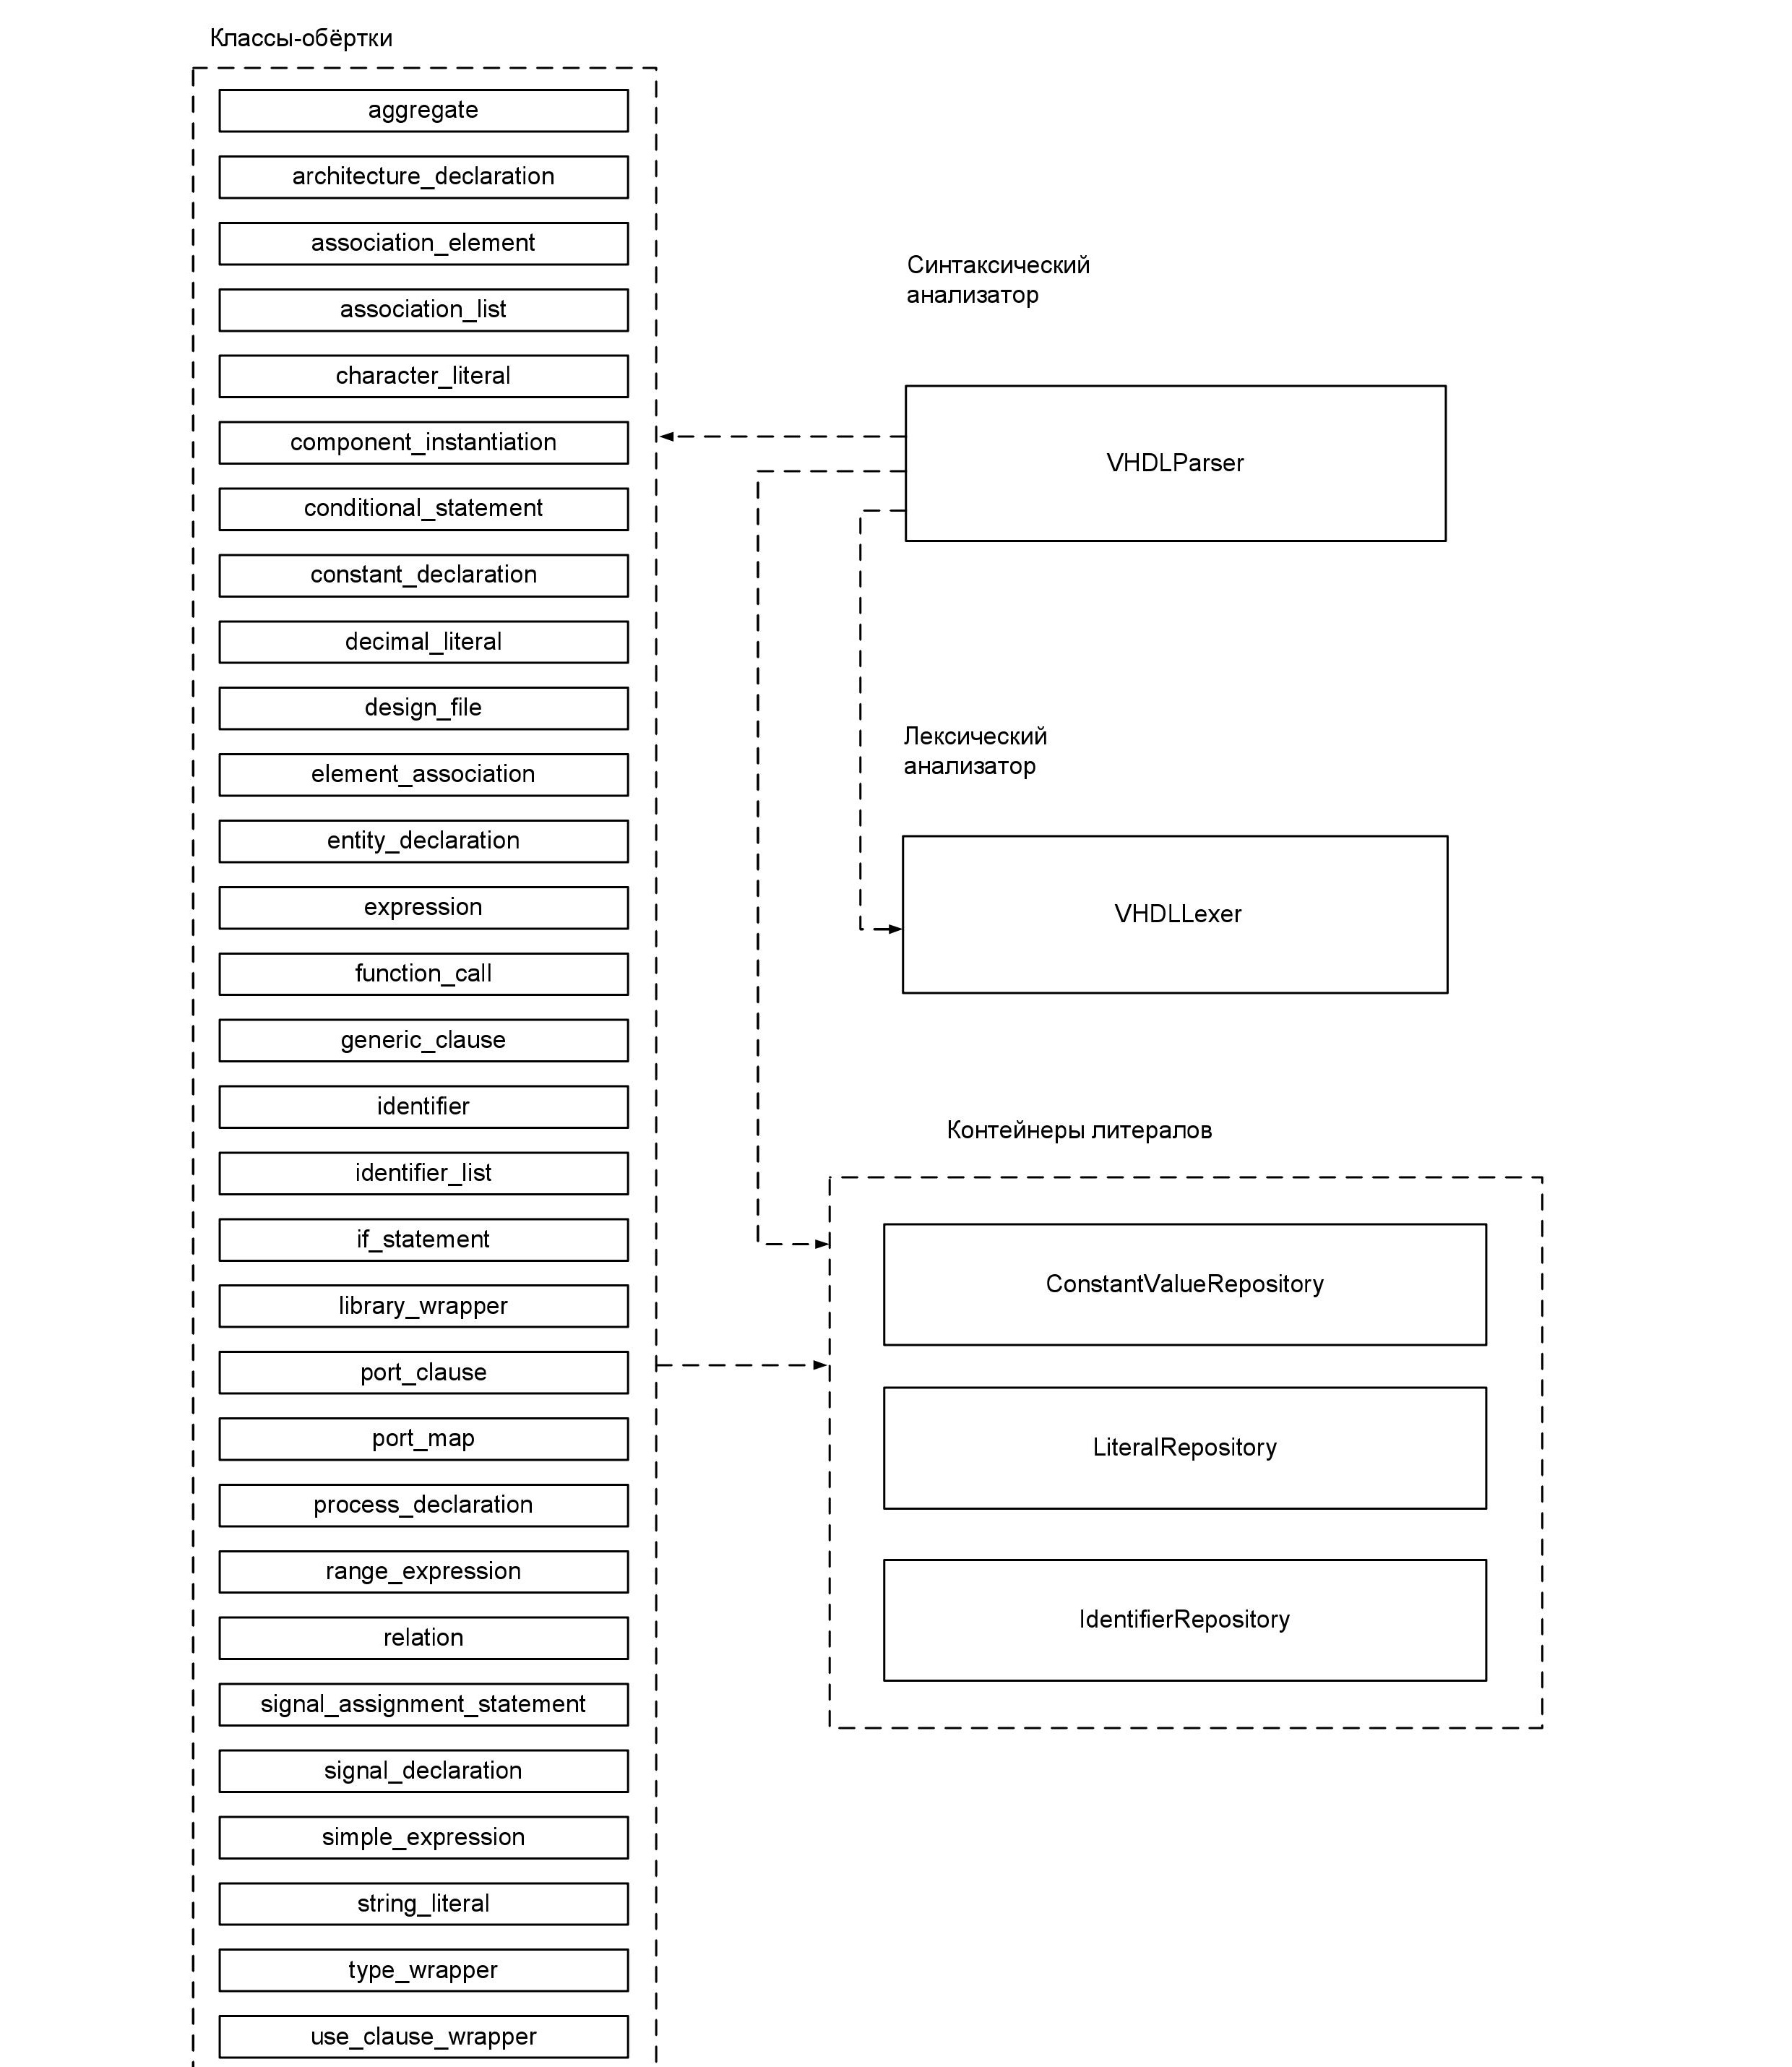
\includegraphics[scale=0.9]{components.jpg}
  \caption{ Диаграмма компонентов программного средства }
  \label{fig:arch_and_mod::components}
\end{figure}


\section{Тестирование приложения}
\label{sec:testing}

Для оценки правильности работы программного средства было проведено тестирование. Тест-кейсы для функционального требования <<Взаимодействие с пользователем>> представлены в таблице \ref{sec:testing:interaction_cases}



\begin{longtable}[l]{| >{\raggedright}m{0.3\textwidth}
                  | >{\raggedright}m{0.3\textwidth}
                  | >{\raggedright\arraybackslash}m{0.3\textwidth}|}
  \caption{Тестирование взаимодействия с пользователем}
  \label{sec:testing:interaction_cases} \tabularnewline

  \hline
       Название тест-кейса и его описание & Ожидаемый результат  & Полученный результат \\
   \hline
   \centering{1} & \centering{2} & \centering{3} \tabularnewline
   \hline
   Запуск программы без аргументов \\ а) Ввести имя исполняемого модуля без аргументов \\ б) нажать клавишу Ввода  &
   a) Имя исполняемого модуля отображается в консоли \\ б) Отображается справочная информация об использовании приложения &
   Пройден \\
   \hline


  Запуск программы с неверными аргументами \\
   а) Ввести имя исполняемого модуля с неверными аргументами \\
   б) Нажать клавишу ввода
   &
   а) Имя исполняемого модуля и аргументы отображаются в консоли \\
   б) Отображается ошибка о вводе неправильного аргумента(аргументов)
   &
   Пройден \\
   \hline

   Запуск программы с неверными аргументами \\
   a) Ввести имя исполняемого модуля с неверными аргументами \\
   б) Нажать клавишу ввода
   &
   а) Имя исполняемого модуля и аргументы отображаются в консоли \\
   б) Отображается ошибка о вводе неправильного аргумента(аргументов)
   &
   Пройден \\
   % \pagebreak

   % \caption*{Продолжение таблицы~\ref{sec:testing:interaction_cases}} \\
   % \hline
   % 1 & 2 & 3 \\
   % \hline

  \pagebreak
  \caption*{Продолжение таблицы~\ref{sec:testing:interaction_cases}} \\
   \hline
   \centering 1 & \centering 2 & \centering 3 \tabularnewline
   \hline

   Запуск программы с переданным путём до существующего файла \\
   a) Ввести имя исполняемого модуля и передать путь до существующего файла как аргумент \\
   б) Нажать клавишу ввода
   % \begin{enumerate}
   % \end{enumerate}
   &
   а) Имя исполняемого модуля с путём до существующего файла отображаются в консоли \\
   б) Программа выводит обфусцированный код в консоль\\
   &
   Пройден\\
   \hline


   Запуск программы с несуществующим файлом \\
   а) Ввести имя исполняемого модуля и передать путь до несуществующего файла как аргумент \\
   б) нажать клавишу Ввода
   &
   а) Имя исполняемого модуля с путём до несуществующего файла отображаются в консоли \\
   б) Программа выводит ошибку о том, что файл не может быть найден
   &
   Пройден \\
   \hline

   Запуск программы с входным и выходным файлом \\
   а) Ввести имя исполняемого модуля и передать путь до существующего файла и файла вывода как аргументы \\
   б) Нажать клавишу Ввода \\
   в) Открыть файл вывода
   &
   а) Имя исполняемого модуля с путём до существующего файла и файла вывода отображаются в консоли \\
   б) Программа выполняет работу \\
   в) Конечный файл содержит результаты работы программы
   &
   Пройден \\
  \pagebreak
  \caption*{Продолжение таблицы~\ref{sec:testing:interaction_cases}} \\
   \hline
   \centering 1 & \centering 2 & \centering 3 \tabularnewline
   \hline
   Запуск программы с входным файлом и флагом --lexical-only
   а) Ввести имя исполняемого модуля и передать путь до существующего файла с аргументов --lexical-only \\
   б) нажать клавишу Ввода
   &
   а) Имя исполняемого модуля с путём до существующего файла и аргумент отображаются в консоли \\
   б) Программа не содержит функциональной обфускации
   &
   Пройден \\
   \hline
   Запуск программы с входным файлом и флагом --functional-only
   а) Ввести имя исполняемого модуля и передать путь до существующего файла с аргументов --functional-only \\
   б) нажать клавишу Ввода
   &
   а) Имя исполняемого модуля с путём до существующего файла и аргумент отображаются в консоли \\
   б) Программа содержит функциональную обфускацию, но не содержит лексической
   &
   Пройден \\
   \hline
\end{longtable}





   Тест-кейсы для функционального требования <<Анализирование входных файлов>> представлены в таблице \ref{sec:testing:analyzing_cases}.
   \pagebreak
\begin{longtable}[l]{| >{\raggedright}m{0.3\textwidth}
                  | >{\raggedright}m{0.3\textwidth}
                  | >{\raggedright\arraybackslash}m{0.3\textwidth}|}
  \caption{Тестирование функциональных требований}
  \label{sec:testing:analyzing_cases} \tabularnewline

  \hline
    Название тест-кейса и его описание & Ожидаемый результат & Полученный результат
    \tabularnewline
   \hline
   \centering 1 & \centering 2 & \centering 3 \tabularnewline
   \hline
   Запуск программы с действительным VHDL кодом \\
   а) Ввести имя исполняемого модуля с входным файлом, являющимся правильным VHDL-кодом \\
   Б) нажать клавишу Ввода
   &
   а) Имя исполняемого модуля и путь до файла отображается в консоли \\
   б) Генерируется правильное абстрактное синтаксическое дерево
   &
   Пройден \\

   \hline
   Запуск программы с недействительным VHDL кодом \\
   а) Ввести имя исполняемого модуля с входным файлом, являющимся неправильным VHDL-кодом \\
   б) нажать клавишу Ввода
   &
   а) Имя исполняемого модуля и путь до файла отображается в консоли \\
   б) Выводится сообщения об ошибке анализа
   &
   Пройден \\
   \hline
\end{longtable}
Таким образом, результат тестирования подтверждает, что программное средство лексической и функциональной обфускации проектных описаний цифровых устройств функционирует в полном соответствии со спецификацией требований.
  % \begin{longtable}[l]{| >{\raggedright}m{0.3\textwidth}
  %                 | >{\centering}m{0.3\textwidth}
  %                 | >{\centering}m{0.3\textwidth}|}
  % \caption{Тестирование анализирования входных файлов}
  % \label{sec:testing:analyzing_cases} \tabularnewline

  % \hline
  %      Название тест-кейса и его описание & Ожидаемый результат & Полученный результат
  %    \tabularnewline
  %  \hline
  %  1 & 2 & 3 \\
  %  \hline
  %  Запуск программы без аргументов
  %  \begin{enumerate}
  %  \item Ввести имя исполняемого модуля без аргументов
  %  \item нажать клавишу Ввода
  %  \end{enumerate}
  %  &
  %  \begin{enumerate}
  %  \item Имя исполняемого модуля отображается в консоли
  %  \item Отображается справочная информация об использовании приложения
  %  \end{enumerate}
  %  &
  %  \begin{enumerate}
  %  \item Имя исполняемого модуля отображается в консоли
  %  \item Отображается справочная информация об использовании приложения
  %  \end{enumerate} \\
  %  \hline
   %-----------------------------------------
  % \caption*{Продолжение таблицы~\ref{table:econ:calculation_cost_and_price}}
  % \hline
  %   {\begin{center}
  %      Наименование статей
  %   \end{center} } & \mbox{Норматив,} \% & Методика расчета & \mbox{Значение,} руб. \\
  %  \hline
   % Прогнозируемая цена без налогов
   % &
   % & $ \text{Ц}_{\text{п}} = \text{С}_{\text{п}} + \text{П}_{\text{с}}$
   % & \num{\estimatedPrice} \\
   % \hline
   % Отчисления и налоги в местный и республиканский бюджеты
   % & $ \text{Н}_{\text{мр}} = \num{\localRepubTaxNormative} $
   % & $ \text{О}_{\text{мр}} = { \text{Ц}_{\text{п}} \cdot \text{Н}_{\text{мр}} } / { \num{100} - \text{Н}_{\text{мр}} } $
   % & \num{\localRepubTax} \\
   % \hline
   % Налог на добавленную стоимость
   % & $ \text{Н}_{\text{дс}} = \num{\ndsNormative} $
   % & $ \text{НДС}_{\text{}} = { (\text{Ц}_{\text{п}} + \text{О}_{\text{мр}}) \cdot \text{Н}_{\text{дс}} } / \num{100} $
   % & \num{\nds} \\
   % \hline
   % Прогнозируемая отпускная цена
   % &
   % & $ \text{Ц}_{\text{о}} = \text{Ц}_{\text{п}} + \text{О}_{\text{мр}} + \text{НДС} $
   % & \num{\sellingPrice} \\
   % \hline


\section{Методика~использования разработанного приложения}
\label{sec:usage}
Программное средство лексической и функциональной обфускации проектных описаний цифровых устройств представляет собой консольное приложение, которое может работать под управлением операционных систем семейства Windows и *nix. Корректная работа приложения гарантируется в ОС, перечисленных в разделе, описывающем анализ предметной области и укрупненную спецификацию требований. Данная методика использования программного сердства составлена с использованием операционной системы Arch Linux и симулятора терминала Sakura. Поскольку приложение является консольным и не содержит промежуточных состояний, в качестве управления используются аргументы, передаваемые при запуске приложения. Запуск приложения без аргументов(или с использованием аргументов -h или -help) и результат его работы представлены на рисунке \ref{fig:sec:usage:without_args}.

При запуске приложения в аналитическом режиме проверяется правильность кода, однако не выполняется его обфускация. Анализатор проверяет каждую сущность в дизайне и если она верна, то выводится соответствующее сообщение:

\begin{figure}[hbtp]
\centering
  
\includegraphics[scale=0.65]{analyze_success.jpg}
  \caption{ Запуск приложения в аналитическом режиме с корректным входным файлом }
  \label{fig:sec:usage:analyze_success}
\end{figure}

\afterpage{
  \begin{landscape}
  \thispagestyle{lscape}
  \begin{figure}[htbp]
  \centering
    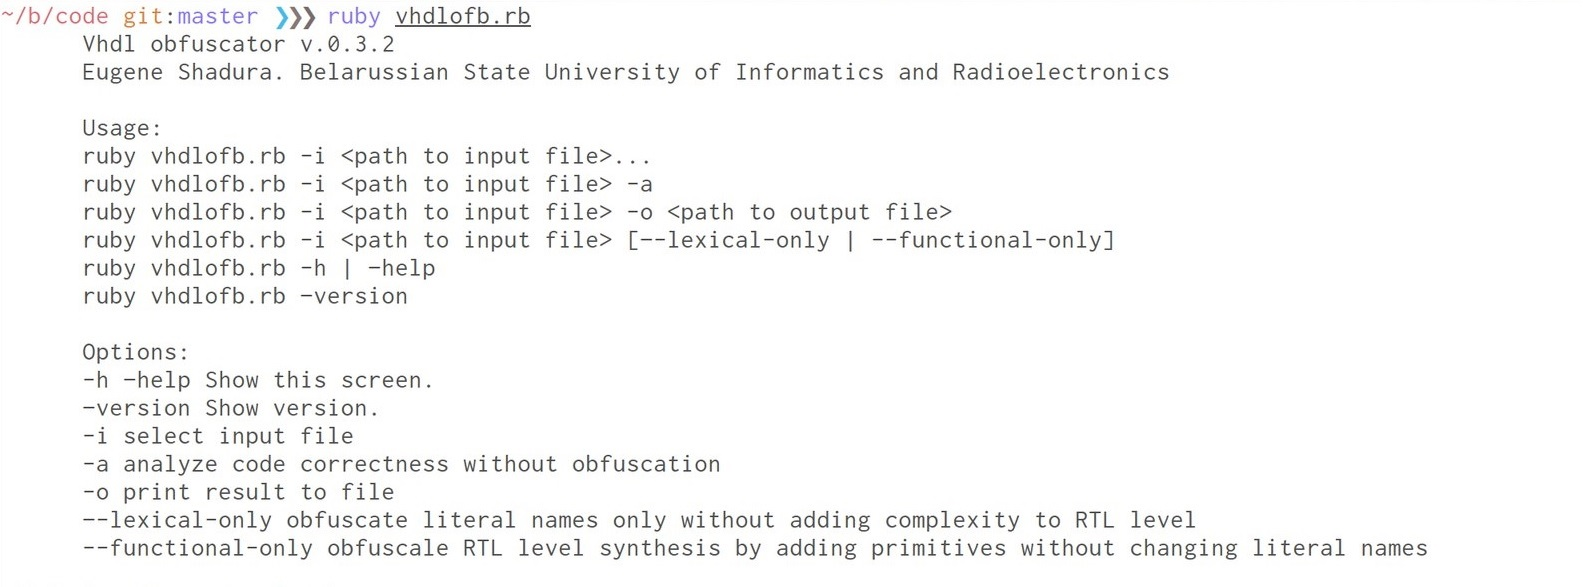
\includegraphics[scale=0.65]{without_args.jpg}
    \caption{ Запуск приложения без аргументов }
    \label{fig:sec:usage:without_args}
  \end{figure}
  \end{landscape}

}

Если же исходный код содержит какие-либо ошибки, то пользователь увидит сообщение с ошибкой, которое содержит символ, который привёл к ней:


\begin{figure}[ht]
\centering
  
\includegraphics[scale=0.65]{analyze_error.jpg}
  \caption{ Запуск приложения в аналитическом режиме с некорректным входным файлом }
  \label{fig:sec:usage:analyze_error}
\end{figure}

\begin{landscape}
\thispagestyle{lscape}
\begin{figure}[ht]
\centering
  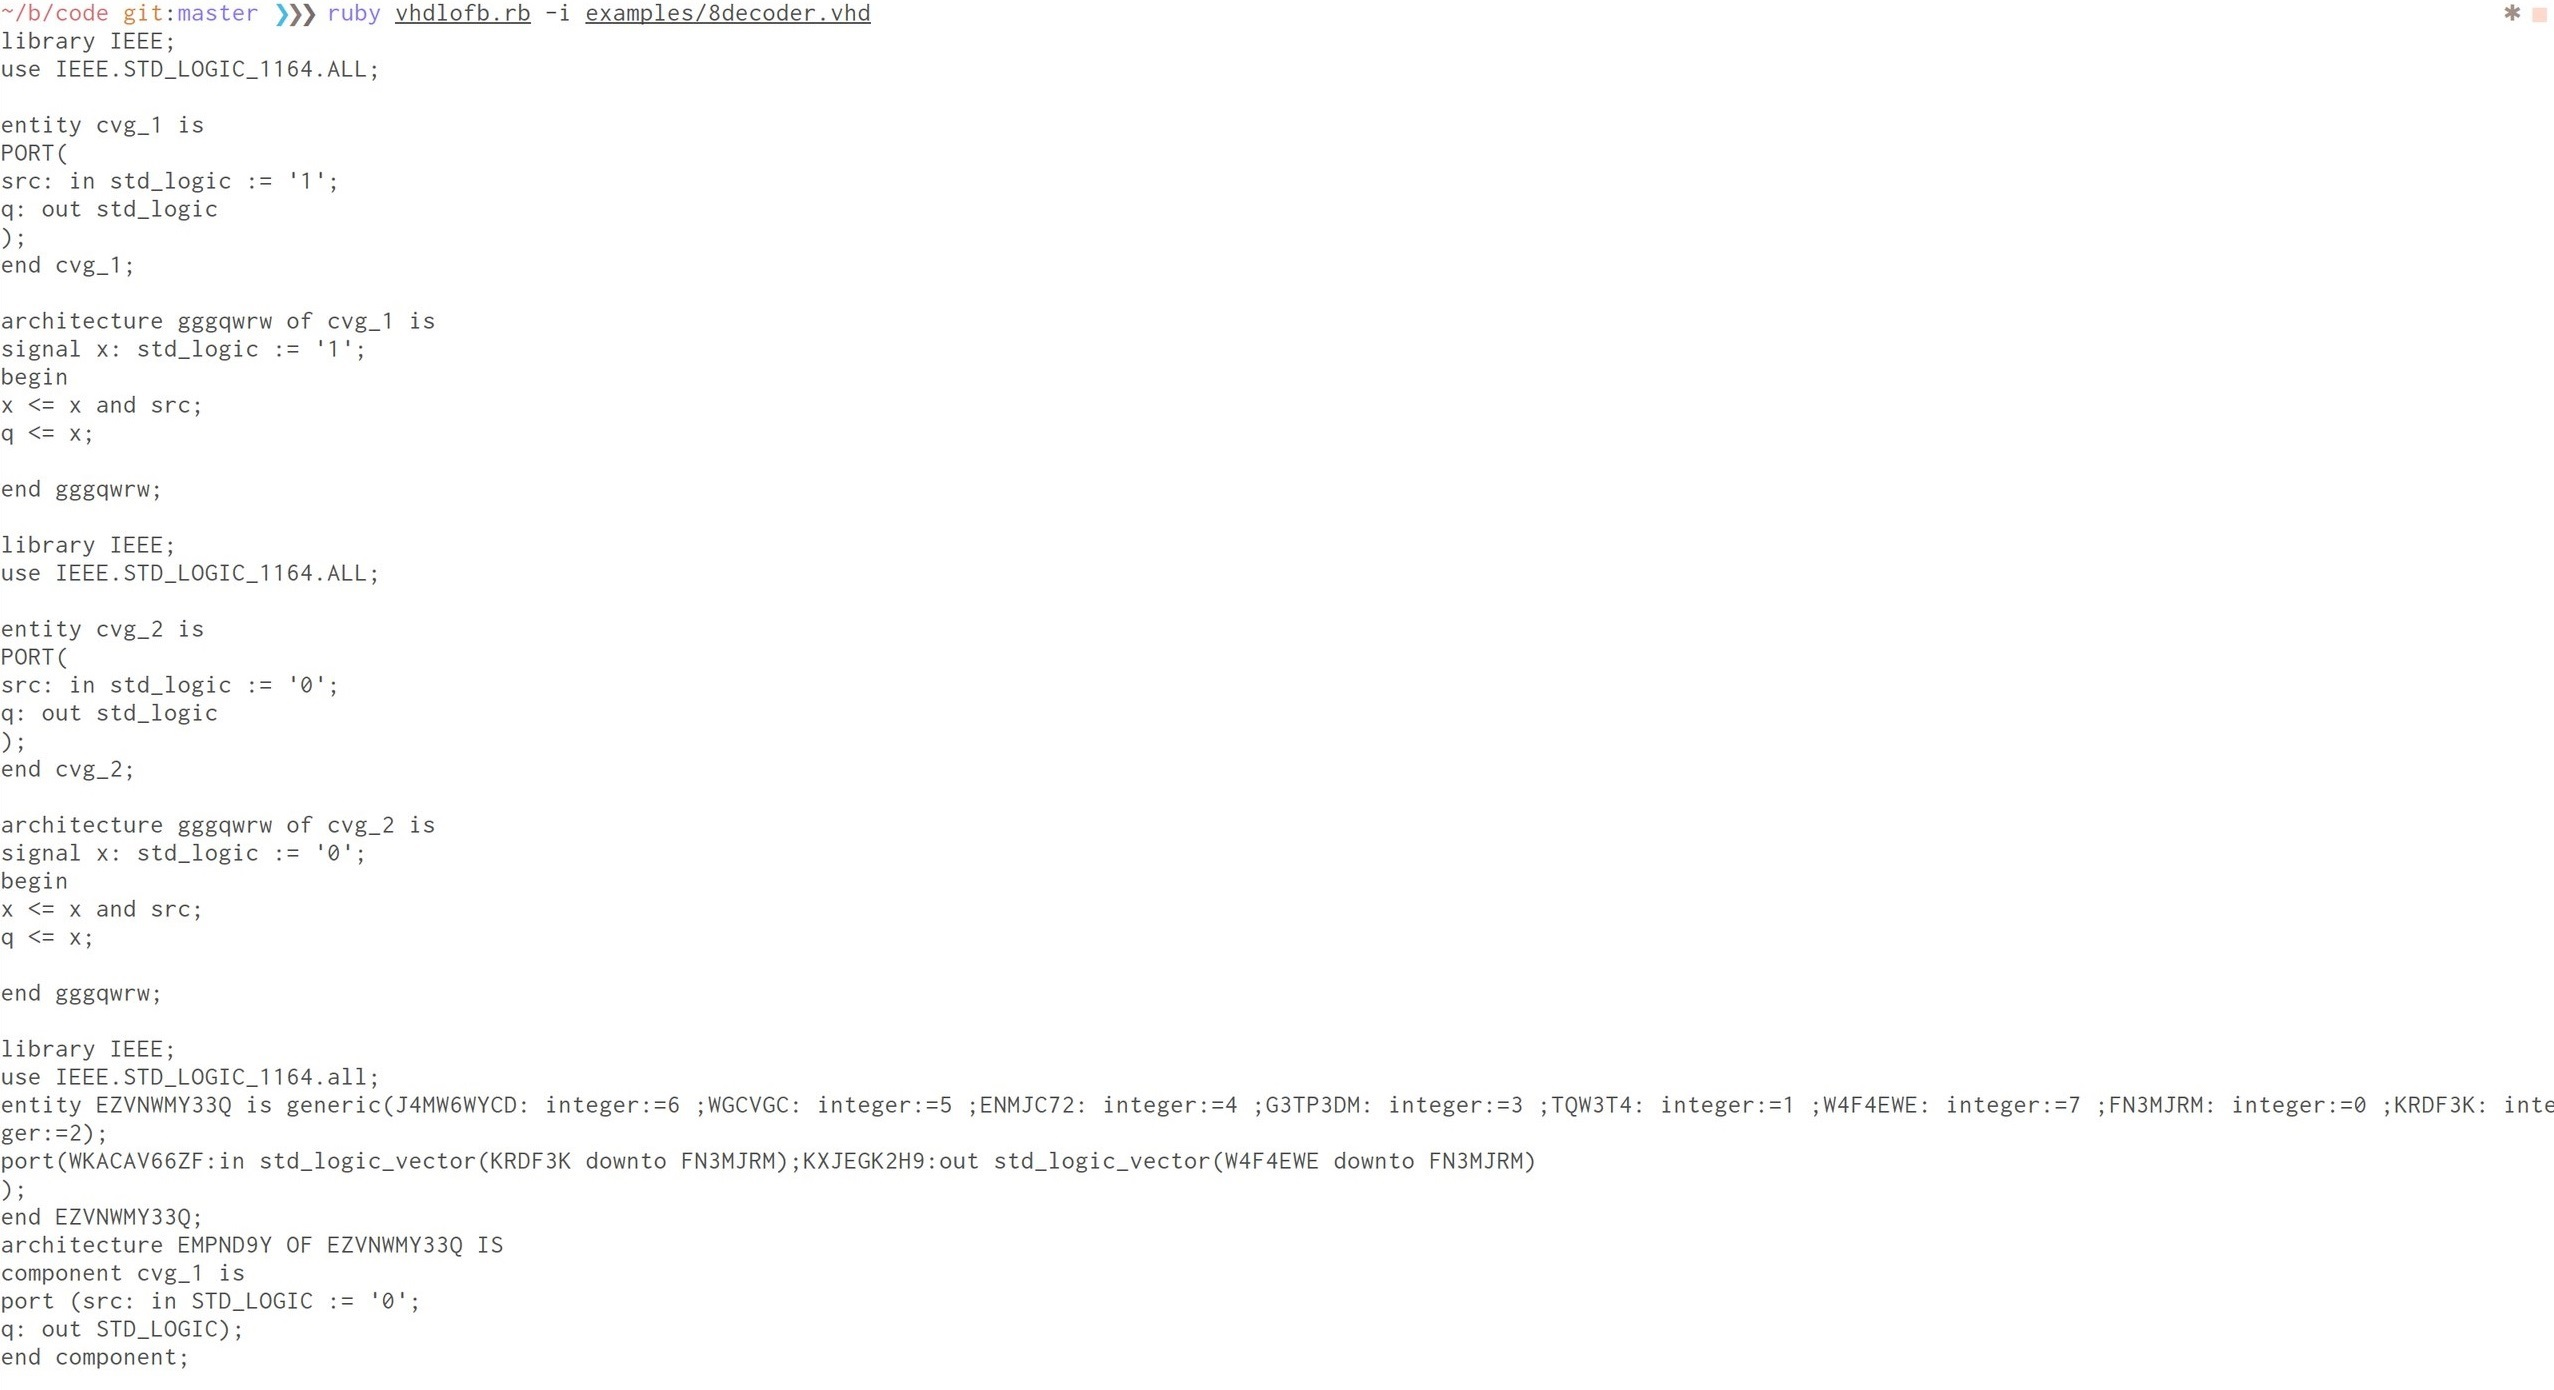
\includegraphics[scale=0.25]{without_output.jpg}
  \caption{ Запуск приложения без указания выходного файла }
  \label{fig:sec:usage:without_output}
\end{figure}
\end{landscape}

\clearpage


% \newcommand{\companyname}{\mbox{<<Техартгруп>>}}

\section{Охрана труда}

\subsection[Обеспечение пожарной безопасности на предприятии]{Обеспечение пожарной безопасности на предприятии малого бизнеса \companyname{}}


Целью дипломного проекта является реализация и анализ алгоритмов построения вероятностных сетей.
Вероятностная сеть является компактным и эффективным способом представления знаний.
Вероятностные сети используются в программном обеспечении для принятия решения в условиях недостаточной определенности.
Данный способ статистического моделирования показал свою пригодность в реальных условиях в сложных предметных областях: медицине, космической промышленности, финансовой сфере и других областях.
Первоначальные стадии разработки дипломного проекта выполнялись на предприятии ООО~\companyname{} во время прохождения преддипломной практики.
В настоящем разделе рассматриваются вопросы, связанные с обеспечением пожарной безопасности на предприятии.

Предприятие \companyname{} занимается предоставлением услуг по разработке информационных систем для иностранных предприятий. 
В минском офисе компании на данный момент работает более 200 человек. 
% TODO: Переписать абсолютный бред в оставшейся части абзаца.
Большое количество конкурирующих компаний, разрабатывающих программное обеспечение в Минске, способствует повышению общего уровня условий труда.
Это, в частности, сказывается на комфортабельности рабочих мест.
Работникам предоставляются светлые, проветриваемые, тихие кабинеты, гибкий график рабочего времени, специальные комнаты отдыха и т.\,д.
Современные компании негласно ориентируются на соответствие лучшим мировым практикам в области охраны труда и, в частности, пожарной безопасности.

На предприятии \companyname{} за пожарную безопасность отвечает директор компании.
Для каждого нового сотрудника производится инструктаж по пожарной безопасности и технике безопасности, а так же знакомство с планом эвакуации при возникновении черезвычайных ситуаций~\cite[\ignore{раздел~5.5.8,} с.~324]{michnuk_2009}.
За проведение инструктажа отвечает специальный человек из отдела материально"=технического снабжения предприятия.
В компании действует набор правил, обязательных для исполнения сотрудниками.
В целях повышения пожарной безопасности курение в здании офиса запрещено.
Все сотрудники обязаны в конце рабочего дня выключить свои персональные компьютеры и обесточить их.
В конце рабочего дня специальный сотрудник проверяет соблюдение данного правила в каждом рабочем кабинете, чтобы там были выключены все электрические приборы: компьютеры, электрические чайники, кондиционеры, освещение и т.\,д.
Все рабочие компьютеры подключены к источникам бесперебойного питания, которые подключены к сетевыми фильтрам, защищающим от скачков напряжения в электросети.

Офис компании расположен в центре города.
Здание офиса представляет собой монолитную железобетонную конструкцию высотой шесть этажей, офис компании находится на двух верхних этажах.
Конструкция здания предусматривает три способа эвакуации с этажа: выход в паркинг, лестничная клетка с выходом на улицу, лестничная клетка с выходом на первый этаж паркинга. 
В случае недоступности основных эвакуационных выходов из каждого кабинета можно через окно попасть на лоджию~\cite[\ignore{раздел~5.5.4,} с.~314\,--\,316]{michnuk_2009}.
Схемы эвакуации выдаются в виде электронного документа каждому новому сотруднику, а также находятся на специальном стенде в рабочих кабинетах.
Все кабинеты офиса расположены вдоль длинного коридора, который оборудован специальными аварийными светильниками и знаками, указывающими направление эвакуации.
На случай отключения электроэнергии компания имеет два дизельных"=генератора, обеспечивающих нужды предприятия на случай отключения электроэнергии.

Офис компании оборудован необходимыми средствами сигнализации о пожаре~\cite[с.~215]{sinilov_2010}. %\cite[с.~5\,--\,7]{sharovar_1979}. 
Каждый кабинет оборудован пожарным дымовым оптико"=электрическим точечным извещателем \mbox{ИП212-02М1} (рисунок~\ref{fig:fire_alarms}).
На предприятии производиться регулярный контроль и проверка работоспособности пожарных извещателей специальным человеком из отдела материально"=технического снабжения предприятия.
В коридорах дополнительно установлены ручные пожарные извещатели \mbox{ИП 5-2Р} (рисунок~\ref{fig:fire_alarms}).
Для извещения о пожаре также может быть использована корпоративная электронная почта, а также другие современные способы обмена информацией.

\begin{figure}[ht]
\centering
  \begin{subfigure}[b]{0.45\textwidth} 
    \centering
    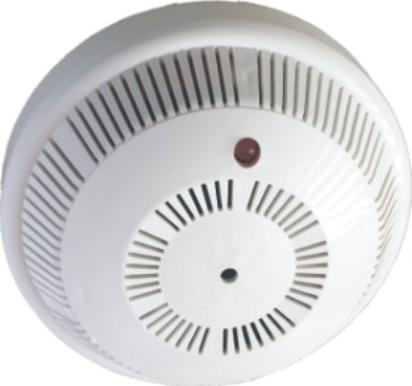
\includegraphics[scale=0.85]{avt_pozh_izv.jpg}  
    \caption{}
  \end{subfigure}
  \begin{subfigure}[b]{0.45\textwidth} 
    \centering
    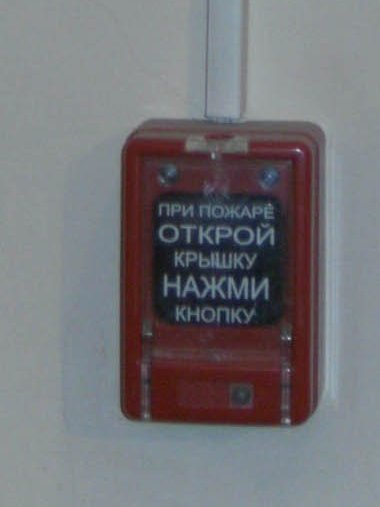
\includegraphics[scale=1.2]{ruch_pozh_izv.jpg}  
    \caption{}
  \end{subfigure}
  \caption{ а "--- автономный пожарный извещатель;
            б "--- ручной пожарный извещатель.}
  \label{fig:fire_alarms}
\end{figure}

На случай возникновения пожара в каждом рабочем кабинете находиться ручной порошковый огнетушитель \mbox{ОП-10}~(з)~МИГ~М (рисунок~\ref{fig:extinguishing_fire}), пригодный для тушения пожаров различного типа, в том числе для тушения электрических приборов~\cite[\ignore{раздел 5.5.7,} с.~221\,--\,323]{michnuk_2009}.
Каждый этаж здания офиса оборудован двумя пожарными кранами для тушения пожара.
Пожарные краны расположены в противоположных частях коридора, недалеко от эвакуационных выходов (рисунок~\ref{fig:extinguishing_fire}).
На случай воспламенения электрической проводки или другого электрического оборудования в каждом кабинете установлены электрические щитки, необходимые для отключения подачи электроэнергии в пределах кабинета.
Во всех помещениях офиса предприятия установлена оросительная система пожаротушения для ликвидации возгорания до приезда пожарной службы~\cite[\ignore{раздел~5.5.6,} с.~318\,--\,320]{michnuk_2009}.
При расследовании возможных причин возникновения пожара может быть задействована система видео"=наблюдения, установленная во всех помещениях предприятия.

\begin{figure}[ht]
\centering
  \begin{subfigure}[b]{0.45\textwidth} 
    \centering
    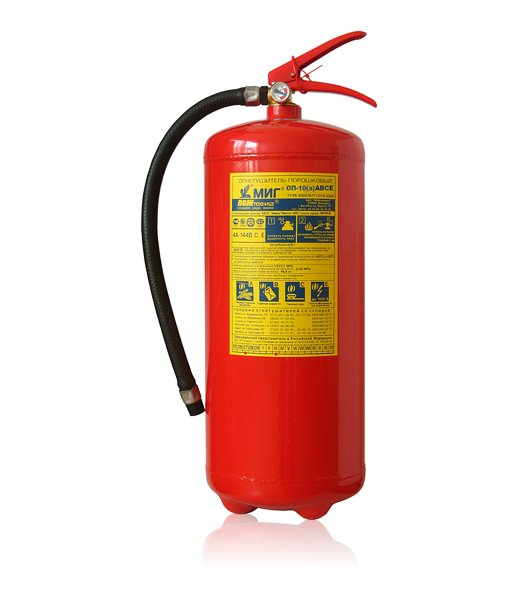
\includegraphics[scale=0.34]{ognetush.jpg}  
    \caption{}
  \end{subfigure}
  \begin{subfigure}[b]{0.45\textwidth} 
    \centering
    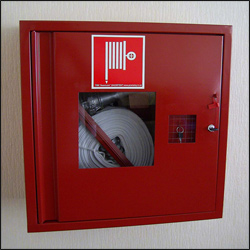
\includegraphics[scale=0.7]{pozh_kran.jpg}  
    \caption{}
  \end{subfigure}
  \caption{ а "--- порошковый огнетушитель \mbox{ОП-10}~(з)~МИГ~М;
            б "--- пожарный кран.}
  \label{fig:extinguishing_fire}
\end{figure}

Основной род деятельности на предприятии "--- разработка информационных систем "--- не предусматривает непосредственный контакт с горючими или легко"=воспламеняющимися веществами, что сильно снижает риски возникновения пожара на предприятии.
Наиболее вероятными причинами возникновения пожара, с учетом специфики предприятия, могут являться нарушение правил внутреннего распорядка "--- курение на рабочем месте, и неисправность электрического оборудования, которого в офисе компании достаточно~\cite[\ignore{раздел 5.5.1,} с.~312]{michnuk_2009}.
С целью снижения риска возникновения пожара по причине неисправности электрического оборудования в компании запрещено пользоваться неисправным оборудованием, а все исправное оборудование подключается в сеть через специальные сетевые фильтры и источники бесперебойного питания.
В целом правила распорядка на предприятии и высокая культура работы с электрическим оборудованием снижают риски возникновения пожара до минимума.

Большой проблемой в достижении максимальной пожарной безопасности предприятия является доступность подъезда пожарной техники к зданию офиса.
В будние дни прилегающие улицы, стоянки, пешеходные переходы заняты неправильно припаркованным личным транспортом.
Большую часть светлого времени суток движение по прилегающим улицам очень затруднено.
Данную проблему предприятие не в силах решить самостоятельно, проблема заключается в низкой культуре владельцев транспорта и игнорировании многочисленных нарушений правил дорожного движения  сотрудниками ГАИ.
% Заключительное предложение
Таким образом, изложенные выше предложения, не смотря на проблемы с подъездом пожарной техники, обеспечат пожарную безопасность на предприятии \companyname{}.


\newcommand{\byr}{Br}

\section{Технико-экономическое обоснование разработки ПС}

% Begin Calculations

\FPeval{\totalProgramSize}{16025}
\FPeval{\totalProgramSizeCorrected}{14490}

\FPeval{\normativeManDays}{306} %Tn

\FPeval{\additionalComplexity}{0.20} %Ksl
\FPeval{\complexityFactor}{clip(1 + \additionalComplexity)}

\FPeval{\stdModuleUsageFactor}{0.9} %Kt
\FPeval{\originalityFactor}{0.7} %Kn

\FPeval{\adjustedManDaysExact}{clip( \normativeManDays * \complexityFactor * \stdModuleUsageFactor * \originalityFactor )}
\FPround{\adjustedManDays}{\adjustedManDaysExact}{0}

\FPeval{\daysInYear}{366}
\FPeval{\redLettersDaysInYear}{6}
\FPeval{\weekendDaysInYear}{105}
\FPeval{\vocationDaysInYear}{24}
\FPeval{\workingDaysInYear}{ clip( \daysInYear - \redLettersDaysInYear - \weekendDaysInYear - \vocationDaysInYear ) }

\FPeval{\developmentTimeMonths}{6}
\FPeval{\developmentTimeYearsExact}{clip(\developmentTimeMonths / 12)}
\FPround{\developmentTimeYears}{\developmentTimeYearsExact}{2}
\FPeval{\requiredNumberOfProgrammersExact}{ clip( \adjustedManDays / (\developmentTimeYears * \workingDaysInYear) + 0.5 ) }

% тут должно получаться 2 ))
\FPtrunc{\requiredNumberOfProgrammers}{\requiredNumberOfProgrammersExact}{0}

\FPeval{\tariffRateFirst}{298000} %Tm1
\FPeval{\tariffFactorFst}{3.04}
\FPeval{\tariffFactorSnd}{3.48}


\FPeval{\employmentFstExact}{clip( \adjustedManDays / \requiredNumberOfProgrammers )}
\FPtrunc{\employmentFst}{\employmentFstExact}{0}

\FPeval{\employmentSnd}{clip(\adjustedManDays - \employmentFst)}


\FPeval{\workingHoursInMonth}{160} %Fr
\FPeval{\salaryPerHourFstExact}{clip( \tariffRateFirst * \tariffFactorFst / \workingHoursInMonth )}
\FPeval{\salaryPerHourSndExact}{clip( \tariffRateFirst * \tariffFactorSnd / \workingHoursInMonth )}
\FPround{\salaryPerHourFst}{\salaryPerHourFstExact}{0}
\FPround{\salaryPerHourSnd}{\salaryPerHourSndExact}{0}

\FPeval{\bonusRate}{1.5}
\FPeval{\workingHoursInDay}{8}
\FPeval{\totalSalaryExact}{clip( \workingHoursInDay * \bonusRate * ( \salaryPerHourFst * \employmentFst + \salaryPerHourSnd * \employmentSnd ) )}
\FPround{\totalSalary}{\totalSalaryExact}{0}

\FPeval{\additionalSalaryNormative}{20}

\FPeval{\additionalSalaryExact}{clip( \totalSalary * \additionalSalaryNormative / 100 )}
\FPround{\additionalSalary}{\additionalSalaryExact}{0}

\FPeval{\socialNeedsNormative}{0.5}
\FPeval{\socialProtectionNormative}{34.5}
\FPeval{\socialProtectionFund}{ clip(\socialNeedsNormative + \socialProtectionNormative) }

\FPeval{\socialProtectionCostExact}{clip( (\totalSalary + \additionalSalary) * \socialProtectionFund / 100 )}
\FPround{\socialProtectionCost}{\socialProtectionCostExact}{0}

\FPeval{\stuffNormative}{3}
\FPeval{\stuffCostExact}{clip( \totalSalary * \stuffNormative / 100 )}
\FPround{\stuffCost}{\stuffCostExact}{0}

\FPeval{\timeToDebugCodeNormative}{15}
%\FPeval{\reducingTimeToDebugFactor}{0.3} %?
\FPeval{\adjustedTimeToDebugCodeNormative}{\timeToDebugCodeNormative}

\FPeval{\oneHourMachineTimeCost}{2400}

\FPeval{\machineTimeCostExact}{ clip( \oneHourMachineTimeCost * \totalProgramSizeCorrected / 100 * \adjustedTimeToDebugCodeNormative ) }
\FPround{\machineTimeCost}{\machineTimeCostExact}{0}

\FPeval{\businessTripNormative}{15}
\FPeval{\businessTripCostExact}{ clip( \totalSalary * \businessTripNormative / 100 ) }
\FPround{\businessTripCost}{\businessTripCostExact}{0}

\FPeval{\otherCostNormative}{20}
\FPeval{\otherCostExact}{clip( \totalSalary * \otherCostNormative / 100 )}
\FPround{\otherCost}{\otherCostExact}{0}

\FPeval{\overheadCostNormative}{100}
\FPeval{\overallCostExact}{clip( \totalSalary * \overheadCostNormative / 100 )}
\FPround{\overheadCost}{\overallCostExact}{0}

\FPeval{\overallCost}{clip( \totalSalary + \additionalSalary + \socialProtectionCost + \stuffCost + \machineTimeCost + \businessTripCost + \otherCost + \overheadCost ) }

\FPeval{\supportNormative}{30}
\FPeval{\softwareSupportCostExact}{clip( \overallCost * \supportNormative / 100 )}
\FPround{\softwareSupportCost}{\softwareSupportCostExact}{0}


\FPeval{\baseCost}{ clip( \overallCost + \softwareSupportCost ) }

\FPeval{\profitability}{35}
\FPeval{\incomeExact}{clip( \baseCost / 100 * \profitability )}
\FPround{\income}{\incomeExact}{0}

\FPeval{\estimatedPrice}{clip( \income + \baseCost )}

\FPeval{\localRepubTaxNormative}{3.9}
\FPeval{\localRepubTaxExact}{clip( \estimatedPrice * \localRepubTaxNormative / (100 - \localRepubTaxNormative) )}
\FPround{\localRepubTax}{\localRepubTaxExact}{0}
%\FPeval{\localRepubTax}{0}

\FPeval{\ndsNormative}{20}
\FPeval{\ndsExact}{clip( (\estimatedPrice + \localRepubTax) / 100 * \ndsNormative )}
\FPround{\nds}{\ndsExact}{0}


\FPeval{\sellingPrice}{clip( \estimatedPrice + \localRepubTax + \nds )}

\FPeval{\taxForIncome}{18}
\FPeval{\incomeWithTaxesExact}{clip(\income * (1 - \taxForIncome / 100))}
\FPround{\incomeWithTaxes}{\incomeWithTaxesExact}{0}

% End Calculations

Целью дипломного проекта является создание программного средства для обфускации исходных кодов проектных описаний, написанныъ на языке VHDL.
Данное программное средство позволяет усложнить чтение злоумышленником как исходных кодов программы(лексическая обфускация), так и результата их синтеза(функциональная обфускация). Данное программное средство обладает рядом достоинств: позволяет проверять правильность исходного кода на предварительном этапе, имеет возможность интеграции с другими инструментами разработки, позволяет проводить только лексическую или только функциональную обфускацию, или обе сразу.

Расчеты выполнены на основе методического пособия~\cite{palicyn_2006}.

\subsection{Расчёт сметы затрат и цены программного продукта}

Целесообразность создания коммерческого ПО требует проведения предварительной экономической оценки и расчета экономического эффекта.
Экономический эффект у разработчика ПО зависит от объёма инвестиций в разработку проекта, цены на готовый программный продукт и количества проданных копий, и проявляется в виде роста чистой прибыли.

Исходные данные для разрабатываемого проекта указаны в таблице~\ref{table:econ:initial_data}.

\begin{table}[!ht]
\caption{Исходные данные}
\label{table:econ:initial_data}
  \centering
  \begin{tabular}{| >{\raggedright}m{0.62\textwidth}
                  | >{\centering}m{0.17\textwidth}
                  | >{\centering\arraybackslash}m{0.13\textwidth}|}
    \hline
    {\begin{center}
      Наименование
    \end{center} } & Условное обозначение & Значение \\
    \hline
    Категория сложности & & 2 \\

    \hline
    Коэффициент сложности, ед. & $ \text{К}_\text{с} $ & \num{\complexityFactor} \\

    \hline
    Степень использования при разработке стандартных модулей, ед. & $ \text{К}_\text{т} $ & \num{\stdModuleUsageFactor} \\

    \hline
    Коэффициент новизны, ед. & $ \text{К}_\text{н} $ & \num{\originalityFactor} \\

    \hline
    Годовой эффективный фонд времени, дн. & $ \text{Ф}_\text{эф} $ & \num{\workingDaysInYear} \\

    \hline
    Продолжительность рабочего дня, ч. & $ \text{Т}_\text{ч} $ & \num{\workingHoursInDay} \\

    \hline
    Месячная тарифная ставка первого разряда, \byr{} & $ \text{Т}_{\text{м}_{1}}$ & \num{\tariffRateFirst} \\

    \hline
    Коэффициент премирования, ед. & $ \text{К} $ & \num{\bonusRate} \\

    \hline
    Норматив дополнительной заработной платы, ед. & $ \text{Н}_\text{д} $ & \num{\additionalSalaryNormative} \\

    \hline
    Норматив отчислений в ФСЗН и обязательное страхование, $\%$ & $ \text{Н}_\text{сз} $ & \num{\socialProtectionFund} \\

    \hline
    Норматив командировочных расходов, $\%$ & $ \text{Н}_\text{к} $ & \num{\businessTripNormative} \\

    \hline
    Норматив прочих затрат, $\%$ & $ \text{Н}_\text{пз} $ & \num{\otherCostNormative} \\

    \hline
    Норматив накладных расходов, $\%$ & $ \text{Н}_\text{рн} $ & \num{\overheadCostNormative} \\

    \hline
    Прогнозируемый уровень рентабельности, $\%$ & $ \text{У}_\text{рп} $ & \num{\profitability} \\

    \hline
    Норматив НДС, $\%$ & $ \text{Н}_\text{дс} $ & \num{\ndsNormative} \\

    \hline
    Норматив налога на прибыль, $\%$ & $ \text{Н}_\text{п} $ & \num{\taxForIncome} \\

    \hline
    Норматив расхода материалов, $\%$ & $ \text{Н}_\text{мз} $ & \num{\stuffNormative} \\

    \hline
    Норматив расхода машинного времени, ч. & $ \text{Н}_\text{мв} $ & \num{\adjustedTimeToDebugCodeNormative} \\

    \hline
    Цена одного часа машинного времени, \byr{} & $ \text{Н}_\text{мв} $ & \num{\oneHourMachineTimeCost} \\

    \hline
    Норматив расходов на сопровождение и адаптацию ПО, $\%$ & $ \text{Н}_\text{рса} $ & \num{\supportNormative} \\
    \hline
  \end{tabular}
\end{table}

На основании сметы затрат и анализа рынка ПО определяется плановая отпускаемая цена.
Для составления сметы затрат на создание ПО необходима предварительная оценка трудоемкости ПО и его объёма.
Расчет объёма программного продукта (количества строк исходного кода) предполагает определение типа программного обеспечения, всестороннее техническое обоснование функций ПО и определение объёма каждой функций.
Согласно классификации типов программного обеспечения~\cite[с.~59,~приложение 1]{palicyn_2006}, разрабатываемое ПО с наименьшей ошибкой можно классифицировать как ПО методo"=ориентированных расчетов.

В данном разделе рассмотрим экономическую эффективность программного средства. Программный комплекс относится ко 2-ой группе сложности. Категория новизны продукта - «В».
Для оценки экономической эффективности разработанного программного средства проводится расчет цены и прибыли от продажи одной системы(программы).

Общий объём программного продукта определяется исходя из количества и объёма функций, реализованных в программе:
\begin{equation}
  \label{eq:econ:total_program_size}
  V_{o} = \sum_{i = 1}^{n} V_{i} \text{\,,}
\end{equation}
\begin{explanation}
где & $ V_{i} $ & объём отдельной функции ПО, LoC; \\
    & $ n $ & общее число функций.
\end{explanation}

На стадии технико-экономического обоснования проекта рассчитать точный объём функций невозможно.
Вместо вычисления точного объёма функций применяются приблизительные оценки на основе данных по аналогичным проектам или по нормативам~\cite[с.~61,~приложение 2]{palicyn_2006}, которые приняты в организации.

\begin{table}[ht]
\caption{Перечень и объём функций программного модуля}
\label{table:econ:function_sizes}
\centering
  \begin{tabular}{| >{\centering}m{0.12\textwidth}
                  | >{\raggedright}m{0.40\textwidth}
                  | >{\centering}m{0.18\textwidth}
                  | >{\centering\arraybackslash}m{0.18\textwidth}|}

  \hline
         \multirow{2}{0.12\textwidth}[-0.5em]{\centering \No{} функции}
       & \multirow{2}{0.40\textwidth}[-0.55em]{\centering Наименование (содержание)}
       & \multicolumn{2}{c|}{\centering Объём функции, LoC} \tabularnewline

  \cline{3-4} &
       & { по каталогу ($ V_{i} $) }
       & { уточненный ($ V_{i}^{\text{у}} $) } \tabularnewline

  \hline
  101 & Организация ввода информации & \num{85} & \num{60} \tabularnewline

  \hline
  102 & Контроль, предварительная обработка и ввод информации & \num{300} & \num{250} \tabularnewline

  \hline
  103 & Анализ входного языка(синтаксический и семантический) & \num{700} & \num{690} \tabularnewline

  \hline
  107 & Синтаксический и семантический анализ входного языка и генерация кодов команд & \num{9000} & \num{7800} \tabularnewline

  \hline
  108 & Процессор языка & \num{3500} & \num{3200} \tabularnewline

  \hline
  109 & Организация ввода/вывода информации с интерактивном режиме & \num{200} & \num{150} \tabularnewline

  \hline
  305 & Обработка файлов & \num{300} & \num{2500} \tabularnewline

  \hline
  309 & Формирование файла & \num{1000} & \num{900} \tabularnewline

  \hline
  506 & Обработка ошибочных и сбойных ситуаций & \num{400} & \num{300} \tabularnewline

  \hline
  507 & Обеспечение интерфейса между компонентами & \num{900} & \num{890} \tabularnewline

  \hline

  % Уточенная оценка вычислялась с помощью R: (+ручной фикс)
  % set.seed(35)
  % locs <- c(100, 520, 2700, 520, 750, 1100, 430, 730, 460, 8370)
  % locs.which.corrected <- rbinom(length(locs), 1, 0.4)
  % locs.corrections <- rnorm(length(locs), mean = -0.25, sd=0.3)
  % locs.correction.factor <- 1 + locs.which.corrected * locs.corrections
  % locs.corrected <- signif(locs * locs.correction.factor, digits = 2)
  % locs.corrected
  % sum(locs)
  % sum(locs.corrected)

  Итог & & {\num{\totalProgramSize}} & {\num{\totalProgramSizeCorrected}} \tabularnewline

  \hline

  \end{tabular}
\end{table}

Перечень и объём функций программного модуля перечислен в таблице~\ref{table:econ:function_sizes}.
По приведенным данным уточненный объём некоторых функций изменился, и общий уточненный объём ПО $ V_{\text{у}} = \SI{\totalProgramSizeCorrected}{\text{LoC}} $.

\subsection{Расчёт нормативной трудоемкости}

На основании общего объема ПО определяется нормативная трудоемкость ($ \text{Т}_\text{н}$) с учетом сложности ПО. Для ПО 2-ой группы сложности, к которой относится разрабатываемый программный продукт, нормативная трудоемкость составит~$ \text{Т}_\text{н} = \SI{\normativeManDays}{\text{чел.} / \text{дн.}}  $

Нормативная трудоемкость служит основой для оценки общей трудоемкости~$ \text{Т}_\text{о} $.
Используем формулу (\ref{eq:econ:effort_common}) для оценки общей трудоемкости для небольших проектов:
\begin{equation}
  \label{eq:econ:effort_common}
  \text{Т}_\text{о} = \text{Т}_\text{н} \cdot
                      \text{К}_\text{с} \cdot
                      \text{К}_\text{т} \cdot
                      \text{К}_\text{н} \text{\,,}
\end{equation}
\begin{explanation}
где & $ \text{К}_\text{с} $ & коэффициент, учитывающий сложность ПО; \\
    & $ \text{К}_\text{т} $ & поправочный коэффициент, учитывающий степень использования при разработке стандартных модулей; \\
    & $ \text{К}_\text{н} $ & коэффициент, учитывающий степень новизны ПО.
\end{explanation}

Дополнительные затраты труда на разработку ПО учитываются через коэффициент сложности, который вычисляется по формуле
\begin{equation}
\label{eq:econ:complexity_coeff}
  \text{К}_{\text{с}} = 1 + \sum_{i = 1}^n \text{К}_{i} \text{\,,}
\end{equation}
\begin{explanation}
где & $ \text{К}_{i} $ & коэффициент, соответствующий степени повышения сложности ПО за счет конкретной характеристики; \\
    & $ n $ & количество учитываемых характеристик.
\end{explanation}

Наличие двух характеристик сложности позволяет~\cite[c.~66, приложение~4, таблица~П.4.2]{palicyn_2006} вычислить коэффициент сложности
\begin{equation}
\label{eq:econ:complexity_coeff_calc}
  \text{К}_{\text{с}} = \num{1} + \num{\additionalComplexity} = \num{\complexityFactor} \text{\,.}
\end{equation}

Разрабатываемое ПО использует стандартные компоненты. Согласно справочным данным~\cite[c.~68,~приложение~4, таблица~П.4.5]{palicyn_2006} коэффициент использования стандартных модулей для разрабатываемого приложения $ \text{К}_\text{т} = \num{\stdModuleUsageFactor} $.
Разрабатываемое ПО не является новым, существуют аналогичные более зрелые разработки у различных компаний и университетов по всему миру.
Влияние степени новизны на трудоемкость создания ПО определяется коэффициентом новизны~---~$ \text{К}_\text{н} $.
Согласно справочным данным~\cite[c.~67, приложение~4, таблица~П.4.4]{palicyn_2006} для разрабатываемого ПО $ \text{К}_\text{н} = \num{\originalityFactor} $.
Подставив приведенные выше коэффициенты для разрабатываемого ПО в формулу~(\ref{eq:econ:effort_common}) получим общую трудоемкость разработки
\begin{equation}
  \label{eq:econ:effort_common_calc}
  \text{Т}_\text{о} = \num{\normativeManDays} \cdot \num{\complexityFactor} \cdot \num{\stdModuleUsageFactor} \cdot \num{\originalityFactor} \approx \SI{\adjustedManDays}{\text{чел.}/\text{дн.}}
\end{equation}

На основе общей трудоемкости и требуемых сроков реализации проекта вычисляется плановое количество исполнителей.
Численность исполнителей проекта рассчитывается по формуле:
\begin{equation}
  \label{eq:econ:num_of_programmers}
  \text{Ч}_\text{р} = \frac{\text{Т}_\text{о}}{\text{Т}_\text{р} \cdot \text{Ф}_\text{эф}} \text{\,,}
\end{equation}
\begin{explanation}
где & $ \text{Т}_\text{о} $ & общая трудоемкость разработки проекта, $ \text{чел.}/\text{дн.} $; \\
    & $ \text{Ф}_\text{эф} $ & эффективный фонд времени работы одного работника в течение года, дн.; \\
    & $ \text{Т}_\text{р} $ & срок разработки проекта, лет.
\end{explanation}

Эффективный фонд времени работы одного разработчика вычисляется по формуле
\begin{equation}
  \label{eq:econ:effective_time_per_programmer}
  \text{Ф}_\text{эф} =
    \text{Д}_\text{г} -
    \text{Д}_\text{п} -
    \text{Д}_\text{в} -
    \text{Д}_\text{о} \text{\,,}
\end{equation}
\begin{explanation}
где & $ \text{Д}_\text{г} $ & количество дней в году, дн.; \\
    & $ \text{Д}_\text{п} $ & количество праздничных дней в году, не совпадающих с выходными днями, дн.; \\
    & $ \text{Д}_\text{в} $ & количество выходных дней в году, дн.; \\
    & $ \text{Д}_\text{п} $ & количество дней отпуска, дн.
\end{explanation}

Согласно данным, приведенным в производственном календаре для пятидневной рабочей недели в 2016 году для Беларуси~\cite{belcalendar_2016}, фонд рабочего времени составит
\begin{equation}
  \text{Ф}_\text{эф} = \num{\daysInYear} - \num{\redLettersDaysInYear} - \num{\weekendDaysInYear} - \num{\vocationDaysInYear} = \SI{\workingDaysInYear}{\text{дн.}}
\end{equation}

Учитывая срок разработки проекта $ \text{Т}_\text{р} = \SI{\developmentTimeMonths}{\text{мес.}} = \SI{\developmentTimeYears}{\text{года}} $, общую трудоемкость и фонд эффективного времени одного работника, вычисленные ранее, можем рассчитать численность исполнителей проекта
\begin{equation}
  \label{eq:econ:num_of_programmers_calc}
  \text{Ч}_\text{р} =
    \frac{\num{\adjustedManDays}}
         {\num{\developmentTimeYears} \cdot \num{\workingDaysInYear}}
    \approx \SI{\requiredNumberOfProgrammers}{\text{рабочих}}.
\end{equation}

Вычисленные оценки показывают, что для выполнения запланированного проекта в указанные сроки необходимо два рабочих.

\subsection{Расчёт основной заработной платы исполнителей}

Информация о работниках перечислена в таблице~\ref{table:econ:programmers}.
\begin{table}[ht]
  \caption{Работники, занятые в проекте}
  \label{table:econ:programmers}
  \begin{tabular}{| >{\centering}m{0.4\textwidth}
                  | >{\centering}m{0.15\textwidth}
                  | >{\centering}m{0.18\textwidth}
                  | >{\centering\arraybackslash}m{0.15\textwidth}|}
   \hline
   Исполнители & Разряд & Тарифный коэффициент & \mbox{Чел./дн.} занятости \\
   \hline
   Программист \Rmnum{1}-категории & $ \num{13} $ & $ \num{\tariffFactorFst} $ & $ \num{\employmentFst} $ \\
   \hline
   Ведущий программист & $ \num{15} $ & $ \num{\tariffFactorSnd} $ & $ \num{\employmentSnd} $ \\
   \hline
  \end{tabular}
\end{table}

Месячная тарифная ставка одного работника вычисляется по формуле
\begin{equation}
  \label{eq:econ:month_salary}
  \text{Т}_\text{ч} =
    \frac {\text{Т}_{\text{м}_{1}} \cdot \text{Т}_{\text{к}} }
          {\text{Ф}_{\text{р}} }  \text{\,,}
\end{equation}
\begin{explanation}
где & $ \text{Т}_{\text{м}_{1}} $ & месячная тарифная ставка 1-го разряда, \byr; \\
    & $ \text{Т}_{\text{к}} $ & тарифный коэффициент, соответствующий установленному тарифному разряду; \\
    & $ \text{Ф}_{\text{р}} $ & среднемесячная норма рабочего времени, час.
\end{explanation}




Подставив данные из таблицы~\ref{table:econ:programmers} в формулу~(\ref{eq:econ:month_salary}), приняв значение тарифной ставки 1-го разряда $ \text{Т}_{\text{м}_{1}} = \SI{\tariffRateFirst}{\text{\byr}} $ и среднемесячную норму рабочего времени $ \text{Ф}_{\text{р}} = \SI{\workingHoursInMonth}{\text{часов}} $ получаем
\begin{equation}
  \label{eq:econ:month_salary_calc1}
  \text{Т}_{\text{ч}}^{\text{прогр. \Rmnum{1}-разр.}} = \frac{ \num{\tariffRateFirst} \cdot \num{\tariffFactorFst} } { \num{\workingHoursInMonth} } = \SI{\salaryPerHourFst}{\text{\byr}/\text{час;}}
\end{equation}
\begin{equation}
  \label{eq:econ:month_salary_calc2}
  \text{Т}_{\text{ч}}^{\text{вед. прогр.}} = \frac{ \num{\tariffRateFirst} \cdot \num{\tariffFactorSnd} } { \num{\workingHoursInMonth} } = \SI{\salaryPerHourSnd}{\text{\byr}/\text{час.}}
\end{equation}

Основная заработная плата исполнителей на конкретное ПО рассчитывается по формуле
\begin{equation}
  \label{eq:econ:total_salary}
  \text{З}_{\text{о}} = \sum^{n}_{i = 1}
                        \text{Т}_{\text{ч}}^{i} \cdot
                        \text{Т}_{\text{ч}} \cdot
                        \text{Ф}_{\text{п}} \cdot
                        \text{К}
                          \text{\,,}
\end{equation}
\begin{explanation}
где & $ \text{Т}_{\text{ч}}^{i} $ & часовая тарифная ставка \mbox{$ i $-го} исполнителя, \byr$/$час; \\
    & $ \text{Т}_{\text{ч}} $ & количество часов работы в день, час; \\
    & $ \text{Ф}_{\text{п}} $ & плановый фонд рабочего времени \mbox{$ i $-го} исполнителя, дн.; \\
    & $ \text{К} $ & коэффициент премирования.
\end{explanation}

Подставив ранее вычисленные значения и данные из таблицы~\ref{table:econ:programmers} в формулу~(\ref{eq:econ:total_salary}) и приняв коэффициент премирования $ \text{К} = \num{\bonusRate} $ получим
\begin{equation}
  \label{eq:econ:total_salary_calc}
  \text{З}_{\text{о}} = (\salaryPerHourFst \cdot \num{\employmentFst} + \salaryPerHourSnd \cdot \num{\employmentSnd}) \cdot \num{\workingHoursInDay} \cdot \num{\bonusRate} = \SI{\totalSalary}{\text{\byr}} \text{\,.}
\end{equation}

Дополнительная заработная плата включает выплаты предусмотренные законодательством от труде и определяется по нормативу в процентах от основной заработной платы
\begin{equation}
  \label{eq:econ:additional_salary}
  \text{З}_{\text{д}} =
    \frac {\text{З}_{\text{о}} \cdot \text{Н}_{\text{д}}}
          {100\%} \text{\,,}
\end{equation}
\begin{explanation}
  где & $ \text{Н}_{\text{д}} $ & норматив дополнительной заработной платы, $ \% $.
\end{explanation}

Приняв норматив дополнительной заработной платы $ \text{Н}_{\text{д}} = \num{\additionalSalaryNormative\%} $ и подставив известные данные в формулу~(\ref{eq:econ:additional_salary}) получим
\begin{equation}
  \label{eq:econ:additional_salary_calc}
  \text{З}_{\text{д}} =
    \frac{\num{\totalSalary} \cdot 20\%}
         {100\%} \approx \SI{\additionalSalary}{\text{\byr}} \text{\,.}
\end{equation}

Расчеты общей суммы расходов и прогнозируемой цены ПО, а также его себестоимости сведены в таблицу~\ref{table:econ:calculation_cost_and_price}.

\begin{longtable}[l]{| >{\raggedright}m{0.27\textwidth}
                  | >{\centering}m{0.16\textwidth}
                  | >{\centering}m{0.35\textwidth}
                  | >{\centering\arraybackslash}m{0.15\textwidth}|}
  \caption{Расчет себестоимости и отпускной цены ПО}
  \label{table:econ:calculation_cost_and_price}

  \hline
    {\begin{center}
       Наименование статей
    \end{center} } & \mbox{Норматив,} \% & Методика расчета & \mbox{Значение,} руб. \\
   \hline
   Отчисления в фонд социальной защиты и обязательного страхования
   & $ \text{Н}_{\text{сз}} = \num{\socialProtectionFund} $
   & $ \text{З}_{\text{сз}} = (\text{З}_{\text{о}} + \text{З}_{\text{д}}) \cdot \text{Н}_{\text{сз}} / {\num{100}} $
   & \num{\socialProtectionCost}\\
   \hline
   Материалы и комплектующие
   & $ \text{Н}_{\text{мз}} = \num{\stuffNormative} $
   & $\text{М} = { \text{З}_{\text{о}} \cdot \text{Н}_{\text{мз}} } / { \num{100} } $
   & \num{\stuffCost} \\
   \hline
   Машинное время
   &
   & $ \text{Р}_{\text{м}} = \text{Ц}_{\text{м}} \cdot \text{V}_{\text{о}} / \num{100} \cdot \text{Н}_{\text{мв}} $
   $ \text{Н}_{\text{мв}} = \num{\timeToDebugCodeNormative}{\text{ машино-часов}}$
   $ \text{Ц}_{\text{м}} = \SI{\oneHourMachineTimeCost}{\text{\byr}} $
   & \num{\machineTimeCost} \\
   \hline
   Расходы на научные командировки
   & $ \text{Н}_{\text{к}} = \num{\businessTripNormative} $
   & $  \text{Р}_{\text{к}} = { \text{З}_{\text{о}} \cdot \text{Н}_{\text{к}} } / \num{100} $
   & \num{\businessTripCost} \\
   \hline
   Прочие прямые расходы
   & $ \text{Н}_{\text{пз}} = \num{\otherCostNormative} $
   & $  \text{П}_{\text{з}} = { \text{З}_{\text{о}} \cdot \text{Н}_{\text{пз}} } / \num{100} $
   & \num{\otherCost} \\
   \hline
   Накладные расходы
   & $ \text{Н}_{\text{рн}} = \num{\overheadCostNormative} $
   & $  \text{Р}_{\text{н}} = { \text{З}_{\text{о}} \cdot \text{Н}_{\text{рн}} } / \num{100} $
   & \num{\overheadCost}\\
   \hline
   Общая сумма расходов по смете
   &
   & $  \text{С}_{\text{р}} = \text{З}_{\text{о}} + \text{З}_{\text{д}} + \text{З}_{\text{сз}} + \text{М} + \text{Р}_{\text{м}} + \text{Р}_{\text{к}} + \text{П}_{\text{з}} + \text{Р}_{\text{н}} $
   & \num{\overallCost}\\
   \hline
   Сопровождение и адаптация ПО
   & $ \text{Н}_{\text{рса}} = \num{\supportNormative} $
   & $  \text{Р}_{\text{са}} = {\text{С}_{\text{р}} \cdot \text{Н}_{\text{рса}} } / { \num{100} } $
   & \num{\softwareSupportCost} \\
   \hline
   Полная себестоимость ПО
   &
   & $ \text{С}_{\text{п}} = \text{С}_{\text{р}} + \text{Р}_{\text{са}} $
   & \num{\baseCost} \\
   \hline
   Прогнозируемая прибыль
   & $ \text{У}_{\text{рп}} = \num{\profitability} $
   & $  \text{П}_{\text{с}} = { \text{С}_{\text{п}} \cdot \text{У}_{\text{рп}} } / \num{100} $
   & \num{\income} \\

   %-----------------------------------------
  \caption*{Продолжение таблицы~\ref{table:econ:calculation_cost_and_price}}
  \hline
    {\begin{center}
       Наименование статей
    \end{center} } & \mbox{Норматив,} \% & Методика расчета & \mbox{Значение,} руб. \\
   \hline
   Прогнозируемая цена без налогов
   &
   & $ \text{Ц}_{\text{п}} = \text{С}_{\text{п}} + \text{П}_{\text{с}}$
   & \num{\estimatedPrice} \\
   \hline
   Отчисления и налоги в местный и республиканский бюджеты
   & $ \text{Н}_{\text{мр}} = \num{\localRepubTaxNormative} $
   & $ \text{О}_{\text{мр}} = { \text{Ц}_{\text{п}} \cdot \text{Н}_{\text{мр}} } / { \num{100} - \text{Н}_{\text{мр}} } $
   & \num{\localRepubTax} \\
   \hline
   Налог на добавленную стоимость
   & $ \text{Н}_{\text{дс}} = \num{\ndsNormative} $
   & $ \text{НДС}_{\text{}} = { (\text{Ц}_{\text{п}} + \text{О}_{\text{мр}}) \cdot \text{Н}_{\text{дс}} } / \num{100} $
   & \num{\nds} \\
   \hline
   Прогнозируемая отпускная цена
   &
   & $ \text{Ц}_{\text{о}} = \text{Ц}_{\text{п}} + \text{О}_{\text{мр}} + \text{НДС} $
   & \num{\sellingPrice} \\
   \hline
\end{longtable}

\subsection{Расчёт экономической эффективности у разработчика}

Важная задача при выборе проекта для финансирования это расчет экономической эффективности проектов и выбор наиболее выгодного проекта.
Разрабатываемое ПО является заказным, т.е. разрабатывается для одного заказчика на заказ. На основании анализа рыночных условий и договоренности с заказчиком об отпускной цене прогнозируемая рентабельность проекта составит $ \text{У}_{\text{рп}} = \num{\profitability\%} $.

Чистую прибыль от реализации проекта можно рассчитать по формуле
\begin{equation}
  \label{eq:econ:income_with_taxes}
  \text{П}_\text{ч} =
    \text{П}_\text{c} \cdot
    \left(1 - \frac{ \text{Н}_\text{п} }{ \num{100\%} } \right) \text{\,,}
\end{equation}
\begin{explanation}
  где & $ \text{Н}_{\text{п}} $ & величина налога на прибыль,~$\%$.
\end{explanation}

Приняв значение налога на прибыль $ \text{Н}_{\text{н}} = \num{\taxForIncome\%} $ и подставив известные данные в формулу~(\ref{eq:econ:income_with_taxes}) получаем чистую прибыль
\begin{equation}
  \label{eq:econ:income_with_taxes_calc}
  \text{П}_\text{ч} =
    \num{\income} \cdot \left( 1 - \frac{\num{\taxForIncome\%}}{100\%} \right) = \SI{\incomeWithTaxes}{\text{\byr}} \text{\,.}
\end{equation}

Программное обеспечение разрабатывалось для одного заказчика в связи с этим экономическим эффектом разработчика будет являться чистая прибыль от реализации~$ \text{П}_\text{ч} $.
Рассчитанные данные приведены в таблице~\ref{table:econ:calculated_data}.

\begin{table}[!ht]
\caption{Рассчитанные данные}
\label{table:econ:calculated_data}
  \centering
  \begin{tabular}{| >{\raggedright}m{0.60\textwidth}
                  | >{\centering}m{0.17\textwidth}
                  | >{\centering\arraybackslash}m{0.15\textwidth}|}
    \hline
    {\begin{center}
      Наименование
    \end{center} } & Условное обозначение & Значение \\
    \hline
    Нормативная трудоемкость, чел.$/$дн. & $ \text{Т}_\text{н} $ & \num{\normativeManDays} \\

    \hline
    Общая трудоемкость разработки, чел.$/$дн. & $ \text{Т}_\text{о} $ & \num{\adjustedManDays} \\

    \hline
    Численность исполнителей, чел. & $ \text{Ч}_\text{р} $ & \num{\requiredNumberOfProgrammers} \\

    \hline
    Часовая тарифная ставка программиста \Rmnum{1}-разряда, \byr{}$/$ч. & $ \text{Т}_{\text{ч}}^{\text{прогр. \Rmnum{1}-разр.}} $ & \num{\salaryPerHourFst} \\

    \hline
    Часовая тарифная ставка ведущего программиста, \byr{}$/$ч. & $ \text{Т}_{\text{ч}}^{\text{вед. прогр.}} $ & \num{\salaryPerHourSnd} \\

    \hline
    Основная заработная плата, \byr{} & $ \text{З}_\text{о} $ & \num{\totalSalary} \\

    \hline
    Дополнительная заработная плата, \byr{} & $ \text{З}_\text{д}$ & \num{\additionalSalary} \\

    \hline
    Отчисления в фонд социальной защиты, \byr{} & $ \text{З}_\text{сз} $ & \num{\socialProtectionCost} \\

    \hline
    Затраты на материалы, \byr{} & $ \text{М} $ & \num{\stuffCost} \\

    \hline
    Расходы на машинное время, \byr{} & $ \text{Р}_\text{м} $ & \num{\machineTimeCost} \\

    \hline
    Расходы на командировки, \byr{} & $ \text{Р}_\text{к} $ & \num{\businessTripCost} \\

    \hline
    Прочие затраты, \byr{} & $ \text{П}_\text{з} $ & \num{\otherCost} \\

    \hline
    Накладные расходы, \byr{} & $ \text{Р}_\text{н} $ & \num{\overheadCost} \\

    \hline
    Общая сумма расходов по смете, \byr{} & $ \text{С}_\text{р} $ & \num{\overallCost} \\

    \hline
    Расходы на сопровождение и адаптацию, \byr{} & $ \text{Р}_\text{са} $ & \num{\softwareSupportCost} \\

    \hline
    Полная себестоимость, \byr{} & $ \text{С}_\text{п} $ & \num{\baseCost} \\

    \hline
    Прогнозируемая прибыль, \byr{} & $ \text{П}_\text{с} $ & \num{\income} \\

    \hline
    НДС, \byr{} & $ \text{НДС} $ & \num{\nds} \\

    \hline
    Прогнозируемая отпускная цена ПО, \byr{} & $ \text{Ц}_\text{о} $ & \num{\sellingPrice} \\

    \hline
    Чистая прибыль, \byr{} & $ \text{П}_\text{ч} $ & \num{\incomeWithTaxes} \\

    \hline
  \end{tabular}
\end{table}

\subsection{Выводы по технико-экономическому обоснованию}

Программное средство лексической и функциональной обфускации проектных описаний цифровых устройств является выгодным программным продуктом.
Чистая прибыль от реализации ПС ($ \text{П}_\text{ч} $ \num{\incomeWithTaxes} рублей) остается организации-разработчику и представляет собой экономический эффект от создания нового программного средства. В итоге было произведено технико-экономическое обоснование разрабатываемого проекта, составлена смета затрат и рассчитана прогнозируемая прибыль, а также показана экономическая целесообразность разработки.


\sectioncentered*{Заключение}
\addcontentsline{toc}{section}{Заключение}

Недвижимость является основой материального производства и имущественного благополучия граждан. Вложение капиталов и сбережений в недвижимость – важнейший экономический процесс рыночной экономики. 

В данном дипломном проекте был рассмотрен вопрос продажи и аренды недвижимости, а также была иследована бизнес область в данной тематике. В рамках дипломного проекта было разработано программное средство веб-приложение для продажи квартир.

В разработанном проекте был использован подход, который предоставляет решения с недвижимостью. Программное средство дает пользователю возможность быстрого поиска необходимой недвижимости. Быстрый способ продать или сдать в аренду свою недвижимость. 

В целом получены хорошие результаты по оптимизации в данной бизнес области. Различные функции программного средства, позволяют сократить объем бумажной работы, а так же существенно сокращают время работы риэлторов. 

В итоге получилось раскрыть тему дипломного проекта и создать в его рамках программное обеспечение.
Но за рамками рассматриваемой темы осталось еще много других бизнес правил и функций, которые можно улучшить или реализовать.

В дальнейшем планируется развивать и довести существующее ПО до полноценного приложения, способное решать более широкий класс задач, возникающих в области недвижимости.

% Зачем: Изменение надписи для списка литературы
% Почему: Пункт 2.8.1 Требований по оформлению пояснительной записки.
\renewcommand{\bibsection}{\sectioncentered*{Cписок использованных источников}}
\phantomsection\pagebreak% исправляет нумерацию в документе и исправляет гиперссылки в pdf
\addcontentsline{toc}{section}{Cписок использованных источников}

% Зачем: Печать списка литературы. База данных литературы - файл bibliography_database.bib
\bibliography{bibliography_database}




\sectioncentered*{ПРИЛОЖЕНИЕ А}
\addcontentsline{toc}{section}{Приложение А Исходный код программного средства.}
\begin{center}
\vspace{-1em}
\textbf{ (обязательное)}

\textbf{Исходный код программного средства}
\end{center}


  \begin{lstlisting}[language=Ruby, style=rubystyle]
class VHDLParser


rule

vhdl : design_file {result = val}

abstract_literal :
  DECIMAL_LITERAL {result = DecimalLiteral.new(val[0]);LiteralRepository.add(result);}
  | BASED_LITERAL {result = val[0]}

access_type_definition :
  ACCESS subtype_indication {result = val}

actual_designator :
  expression {result = val[0]}
  | signal_name {result = val[0]}
  | variable_name {result = val[0]}
  | file_name {result = val[0]}
  | OPEN {result = val[0]}

actual_parameter_part :
  parameter_association_list {result = val}

actual_part :
  actual_designator {result = val[0];}
  | function_name '(' actual_designator ')' {result = val;}
  | type_mark '(' actual_designator ')' {result = val;}

adding_operator :
  '+' {result = val}
  | '-' {result = val}
  | '&' {result = val}

aggregate :
  '(' element_association aggregate_loop0 ')' {result = Aggregate.new(val[1..2].flatten);}

aggregate_loop0 :
  ',' element_association aggregate_loop0 {result = val}
  | {result = val}

alias_declaration :
  ALIAS alias_designator ':' subtype_indication IS name signature ';' {result = val}
  | ALIAS alias_designator IS name signature ';' {result = val}
  | ALIAS alias_designator ':' subtype_indication IS name ';' {result = val}
  | ALIAS alias_designator IS name ';' {result = val}

alias_designator :
  identifier {result = val}
  | CHARACTER_LITERAL {result = CharacterLiteral.new(val[0]); ConstantValueRepository.add(result); }
  | operator_symbol {result = val}

allocator :
  NEW subtype_indication {result = val}
  | NEW qualified_expression {result = val}

architecture_body :
    ARCHITECTURE identifier OF type_name IS architecture_declarative_part BEGIN architecture_statement_part END ARCHITECTURE identifier ';' {InitializeRepository.add(val[1]); result = ArchitectureDeclaration.new(val[1], val[3], val[5], val[7],val[9...val.length-1]);}
  | ARCHITECTURE identifier OF type_name IS architecture_declarative_part BEGIN architecture_statement_part END identifier ';' {InitializeRepository.add(val[1]); result = ArchitectureDeclaration.new(val[1], val[3], val[5], val[7],val[9...val.length-1]); }
  | ARCHITECTURE identifier OF type_name IS architecture_declarative_part BEGIN architecture_statement_part END ARCHITECTURE ';' {InitializeRepository.add(val[1]);result = ArchitectureDeclaration.new(val[1], val[3], val[5], val[7],val[9...val.length-1]);}
  | ARCHITECTURE identifier OF type_name IS architecture_declarative_part BEGIN architecture_statement_part END ';' {InitializeRepository.add(val[1]);result = ArchitectureDeclaration.new(val[1], val[3], val[5], val[7],val[9...val.length-1]);}

architecture_declarative_part :
  architecture_declarative_part_loop0 {result = val[0];}

architecture_declarative_part_loop0 :
  block_declarative_item architecture_declarative_part_loop0 {result = val.flatten.compact;}
  | {result = val}

architecture_statement_part :
  architecture_statement_part_loop0 {result = val}

architecture_statement_part_loop0 :
  concurrent_statement architecture_statement_part_loop0 {result = val}
  | {result = val;}

array_type_definition :
  unconstrained_array_definition {result = val}
  | constrained_array_definition {result = val}

assertion :
  ASSERT condition REPORT expression SEVERITY expression {result = val}
  | ASSERT condition SEVERITY expression {result = val}
  | ASSERT condition REPORT expression {result = val}
  | ASSERT condition {result = val}

assertion_statement :
  LABEL ':' assertion ';' {result = val}
  | assertion ';' {result = val}

association_element :
  formal_part '=>' actual_part {result = AssociationElement.new(val[0], val[2]);}
  | actual_part {result = AssociationElement.new(nil, val[0])}

association_list :
  association_element association_list_loop0 {result = AssociationList.new(val.flatten)}

association_list_loop0 :
  ',' association_element association_list_loop0 {result = val[1..2];}
  | {result = val;}

attribute_declaration :
  ATTRIBUTE identifier ':' type_mark ';' {result = val}

attribute_designator :
  attribute_simple_name {result = val}

attribute_name :
  prefix signature '\'' attribute_designator '(' expression ')' {result = val; }
  | prefix '\'' attribute_designator '(' expression ')' {result = val}
  | prefix signature '\'' attribute_designator {result = val}
  | prefix '\'' attribute_designator {result = val}

attribute_simple_name :
  label {result = val[0]; InitializeRepository.add(result)}

attribute_specification :
  ATTRIBUTE attribute_designator OF entity_specification IS expression ';' {result = val}

base_unit_declaration :
  identifier ';' {result = val}

basic_character :
  basic_graphic_character {result = val}
  | format_effector {result = val}

basic_graphic_character :
  upper_case_letter {result = val}
  | digit {result = val}
  | special_character {result = val}
  | space_character {result = val}

binding_indication :
  USE entity_aspect generic_map_aspect port_map_aspect {result = val}
  | generic_map_aspect port_map_aspect {result = val}
  | USE entity_aspect port_map_aspect {result = val}
  | port_map_aspect {result = val}
  | USE entity_aspect generic_map_aspect {result = val}
  | generic_map_aspect {result = val}
  | USE entity_aspect {result = val}
  | {result = val}

block_configuration :
  FOR block_specification block_configuration_loop0 block_configuration_loop1 END FOR ';' {result = val}

block_configuration_loop0 :
  use_clause block_configuration_loop0 {result = val}
  | {result = val}

block_configuration_loop1 :
  configuration_item block_configuration_loop1 {result = val}
  | {result = val}

block_declarative_item :
  subprogram_declaration {result = val}
  | subprogram_body {result = val}
  | type_declaration {result = val}
  | subtype_declaration {result = val}
  | constant_declaration {result = val[0]; }
  | signal_declaration {result = val[0]; result.type.append_semicolon = true}
  | shared_variable_declaration {result = val}
  | file_declaration {result = val}
  | alias_declaration {result = val}
  | component_declaration {result = val}
  | attribute_declaration {result = val}
  | attribute_specification {result = val}
  | configuration_specification {result = val}
  | disconnection_specification {result = val}
  | use_clause {result = val}
  | group_template_declaration {result = val}
  | group_declaration {result = val}

block_declarative_part :
  block_declarative_part_loop0 {result = val}

block_declarative_part_loop0 :
  block_declarative_item block_declarative_part_loop0 {result = val}
  | {result = val}

block_header :
  generic_clause generic_map_aspect ';' port_clause port_map_aspect ';' {result = val}
  | generic_clause port_clause port_map_aspect ';' {result = val}
  | port_clause port_map_aspect ';' {result = val}
  | generic_clause generic_map_aspect ';' port_clause {result = val}
  | generic_clause port_clause {result = val}
  | port_clause {result = val}
  | generic_clause generic_map_aspect ';' {result = val}
  | generic_clause {result = val}
  | {result = val}

block_specification :
  architecture_name {result = val}
  | block_statement_label {result = val}
  | generate_statement_label '(' index_specification ')' {result = val}
  | generate_statement_label {result = val}

block_statement :
  block_label ':' BLOCK '(' guard_expression ')' IS block_header block_declarative_part BEGIN block_statement_part END BLOCK block_label ';' {result = val}
  | block_label ':' BLOCK IS block_header block_declarative_part BEGIN block_statement_part END BLOCK block_label ';' {result = val}
  | block_label ':' BLOCK '(' guard_expression ')' block_header block_declarative_part BEGIN block_statement_part END BLOCK block_label ';' {result = val}
  | block_label ':' BLOCK block_header block_declarative_part BEGIN block_statement_part END BLOCK block_label ';' {result = val}
  | block_label ':' BLOCK '(' guard_expression ')' IS block_header block_declarative_part BEGIN block_statement_part END BLOCK ';' {result = val}
  | block_label ':' BLOCK IS block_header block_declarative_part BEGIN block_statement_part END BLOCK ';' {result = val}
  | block_label ':' BLOCK '(' guard_expression ')' block_header block_declarative_part BEGIN block_statement_part END BLOCK ';' {result = val}
  | block_label ':' BLOCK block_header block_declarative_part BEGIN block_statement_part END BLOCK ';' {result = val}

block_statement_part :
  block_statement_part_loop0 {result = val}

block_statement_part_loop0 :
  concurrent_statement block_statement_part_loop0 {result = val}
  | {result = val}

case_statement :
  case_label ':' CASE expression IS case_statement_alternative case_statement_loop0 END CASE case_label ';' {result = val;}
  | CASE expression IS case_statement_alternative case_statement_loop0 END CASE case_label ';' {result = val;}
  | case_label ':' CASE expression IS case_statement_alternative case_statement_loop0 END CASE ';' {result = val;}
  | CASE expression IS case_statement_alternative case_statement_loop0 END CASE ';' {result = val.join(' ');}

case_statement_alternative :
  WHEN choices '=>' sequence_of_statements {result = val;}

case_statement_loop0 :
  case_statement_alternative case_statement_loop0 {result = val}
  | {result = val}

choice :
  simple_expression {result = val}
  | discrete_range {result = val}
  | element_simple_name {result = val}
  | OTHERS {result = val}

choices :
  choice choices_loop0 {result = val[0]}

choices_loop0 :
  '|' choice choices_loop0 {result = val}
  | {result = val}

component_configuration :
  FOR component_specification binding_indication ';' block_configuration END FOR ';' {result = val}
  | FOR component_specification block_configuration END FOR ';' {result = val}
  | FOR component_specification binding_indication ';' END FOR ';' {result = val}
  | FOR component_specification END FOR ';' {result = val}

component_declaration :
  COMPONENT identifier IS local_generic_clause formal_port_clause END COMPONENT component_simple_name ';' {result = val}
  | COMPONENT identifier local_generic_clause formal_port_clause END COMPONENT component_simple_name ';' {result = val}
  | COMPONENT identifier IS formal_port_clause END COMPONENT component_simple_name ';' {result = val}
  | COMPONENT identifier formal_port_clause END COMPONENT component_simple_name ';' {result = val}
  | COMPONENT identifier IS local_generic_clause END COMPONENT component_simple_name ';' {result = val}
  | COMPONENT identifier local_generic_clause END COMPONENT component_simple_name ';' {result = val}
  | COMPONENT identifier IS END COMPONENT component_simple_name ';' {result = val}
  | COMPONENT identifier END COMPONENT component_simple_name ';' {result = val}
  | COMPONENT identifier IS local_generic_clause formal_port_clause END COMPONENT ';' {result = val}
  | COMPONENT identifier local_generic_clause formal_port_clause END COMPONENT ';' {result = val}
  | COMPONENT identifier IS formal_port_clause END COMPONENT ';' {result = val}
  | COMPONENT identifier formal_port_clause END COMPONENT ';' {result = val}
  | COMPONENT identifier IS local_generic_clause END COMPONENT ';' {result = val}
  | COMPONENT identifier local_generic_clause END COMPONENT ';' {result = val}
  | COMPONENT identifier IS END COMPONENT ';' {result = val}
  | COMPONENT identifier END COMPONENT ';' {result = val}

component_instantiation_statement :
  attribute_simple_name ':' instantiated_unit generic_map_aspect port_map_aspect ';' {result = ComponentInstantiation.new(val[0], val[2], val[3], val[4]);}
  | attribute_simple_name ':' instantiated_unit port_map_aspect ';' {result = ComponentInstantiation.new(val[0], val[2], nil, val[3]);}
  | attribute_simple_name ':' instantiated_unit generic_map_aspect ';' {result = ComponentInstantiation.new(val[0], val[2], val[3], nil); }
  | attribute_simple_name ':' instantiated_unit ';' {result = ComponentInstantiation.new(val[0], val[2], nil, nil); }

component_specification :
  instantiation_list ':' type_name {result = val;}

composite_type_definition :
  array_type_definition {result = val}
  | record_type_definition {result = val}

concurrent_assertion_statement :
  LABEL ':' POSTPONED assertion ';' {result = val}
  | POSTPONED assertion ';' {result = val}
  | LABEL ':' assertion ';' {result = val}
  | assertion ';' {result = val}

concurrent_procedure_call_statement :
  LABEL ':' POSTPONED procedure_call ';' {result = val}
  | POSTPONED procedure_call ';' {result = val}
  | LABEL ':' procedure_call ';' {result = val}
  | procedure_call ';' {result = val}

concurrent_signal_assignment_statement :
  LABEL ':' POSTPONED conditional_signal_assignment {result = val}
  | POSTPONED conditional_signal_assignment {result = val}
  | LABEL ':' conditional_signal_assignment {result = val}
  | conditional_signal_assignment {result = val}
  | LABEL ':' POSTPONED selected_signal_assignment {result = val}
  | POSTPONED selected_signal_assignment {result = val}
  | LABEL ':' selected_signal_assignment {result = val}
  | selected_signal_assignment {result = val}

concurrent_statement :
  block_statement {result = val; }
  | component_instantiation_statement {result = val;}
  | concurrent_procedure_call_statement {result = val; }
  | concurrent_assertion_statement {result = val; }
  | concurrent_signal_assignment_statement {result = val;}
  | process_statement {result = val[0]}
  | generate_statement {result = val;}
  | signal_assignment_statement {result = val[0]}
  |conditional_signal_assignment {result = val[0]}


condition :
  boolean_expression {result = val;}
  | function_call {result = ConditionalStatement.new(val[0], nil, nil);}
  | expression relational_operator expression {result=ConditionalStatement.new(val[0], val[1], val[2]);val;}
  | expression {result=ConditionalStatement.new(val[0], nil, nil);}
  | relation { val = val.flatten; result = ConditionalStatement.new(val[0], val[1], val[2]);val; }

condition_clause :
  UNTIL condition {result = val}

conditional_signal_assignment :
  target '<=' options conditional_waveforms ';' {result = val.flatten.join(' ')}
  | target '<=' conditional_waveforms ';'{result = val.flatten.join(' ')}
  | function_call '<=' conditional_waveforms ';' {result = val.flatten.join(' ')}

conditional_waveforms :
  conditional_waveforms_loop0 waveform WHEN condition {result = val; ; }
  | conditional_waveforms_loop0 waveform {result = val; }
  | conditional_waveforms_loop0 {result = val; }

conditional_waveforms_loop0 :
  waveform WHEN condition ELSE conditional_waveforms_loop0 {result = val.flatten}
  | waveform {result = val[0]}
  | {result = val;}

configuration_declaration :
  CONFIGURATION identifier OF type_name IS configuration_declarative_part block_configuration END CONFIGURATION configuration_simple_name ';' {result = val}
  | CONFIGURATION identifier OF type_name IS configuration_declarative_part block_configuration END configuration_simple_name ';' {result = val}
  | CONFIGURATION identifier OF type_name IS configuration_declarative_part block_configuration END CONFIGURATION ';' {result = val}
  | CONFIGURATION identifier OF type_name IS configuration_declarative_part block_configuration END ';' {result = val}

configuration_declarative_item :
  use_clause {result = val}
  | attribute_specification {result = val}
  | group_declaration {result = val}

configuration_declarative_part :
  configuration_declarative_part_loop0 {result = val}

configuration_declarative_part_loop0 :
  configuration_declarative_item configuration_declarative_part_loop0 {result = val}
  | {result = val}

configuration_item :
  block_configuration {result = val}
  | component_configuration {result = val}

configuration_specification :
  FOR component_specification binding_indication ';' {result = val}

constant_declaration :
  CONSTANT identifier_list ':' subtype_indication ':=' expression ';' {result = ConstantDeclaration.new(val[1], val[3], val[5]); }
  | CONSTANT identifier_list ':' subtype_indication ';' {result = ConstantDeclaration.new(val[1], val[3], nil);}

constrained_array_definition :
  ARRAY index_constraint OF element_subtype_indication {result = val}

constraint :
  range_constraint {result = val}
  | index_constraint {result = val}

context_clause :
  context_clause_loop0 {result = val}

context_clause_loop0 :
  context_item context_clause_loop0 {result = val}
  | {result = val}

context_item :
  library_clause {result = val.flatten;}
  | use_clause {result = val.flatten;}

declaration :
  type_declaration {result = val}
  | subtype_declaration {result = val}
  | object_declaration {result = val}
  | interface_declaration {result = val}
  | alias_declaration {result = val}
  | attribute_declaration {result = val}
  | component_declaration {result = val}
  | group_template_declaration {result = val}
  | group_declaration {result = val}
  | entity_declaration {result = val}
  | configuration_declaration {result = val}
  | subprogram_declaration {result = val}
  | package_declaration {result = val}

delay_mechanism :
  TRANSPORT {result = val}
  | REJECT time_expression INERTIAL {result = val}
  | INERTIAL {result = val}

design_file :
  design_unit design_file_loop0 {result = DesignFile.new(val.flatten)}

design_file_loop0 :
  design_unit design_file_loop0 {result = val}
  | {result = val}

design_unit :
  context_clause library_unit  {result = val}

designator :
  identifier {result = val}
  | operator_symbol {result = val}

direction :
  TO {result = val;}
  | DOWNTO {result = val}

disconnection_specification :
  DISCONNECT guarded_signal_specification AFTER time_expression ';' {result = val}

discrete_range :
  discrete_subtype_indication {result = val}
  | range_expression {result = val}

element_association :
  choices '=>' expression {val[2] = val[2].as_value;result = ElementAssociation.new(val[0], val[2]);}
  | expression {result = ElementAssociation.new([val[0]], val[2]);}

element_declaration :
  identifier_list ':' element_subtype_definition ';' {result = val}

element_subtype_definition :
  subtype_indication {result = val}

entity_aspect :
  ENTITY type_name '(' architecture_identifier ')' {result = val}
  | ENTITY type_name {result = val}
  | CONFIGURATION configuration_name {result = val}
  | OPEN {result = val}

entity_class :
  ENTITY {result = val}
  | ARCHITECTURE {result = val}
  | CONFIGURATION {result = val}
  | PROCEDURE {result = val}
  | FUNCTION {result = val}
  | PACKAGE {result = val}
  | TYPE {result = val}
  | SUBTYPE {result = val}
  | CONSTANT {result = val}
  | SIGNAL {result = val}
  | VARIABLE {result = val}
  | COMPONENT {result = val}
  | LABEL {result = val}
  | LITERAL {result = val}
  | UNITS {result = val}
  | GROUP {result = val}
  | FILE {result = val}

entity_class_entry :
  entity_class '<>' {result = val}
  | entity_class {result = val}

entity_class_entry_list :
  entity_class_entry entity_class_entry_list_loop0 {result = val}

entity_class_entry_list_loop0 :
  ',' entity_class_entry entity_class_entry_list_loop0 {result = val}
  | {result = val}

entity_declaration :
  ENTITY identifier IS entity_header entity_declarative_part BEGIN entity_statement_part END ENTITY type_name ';' { InitializeRepository.add(val[1]) ;result = EntityDeclaration.new(val[1], val[3], val[4].flatten);}
  | ENTITY identifier IS entity_header entity_declarative_part END ENTITY type_name ';' { InitializeRepository.add(val[1]) ;result = EntityDeclaration.new(val[1], val[3], val[4].flatten);}
  | ENTITY identifier IS entity_header entity_declarative_part BEGIN entity_statement_part END type_name ';' { InitializeRepository.add(val[1]) ;result = EntityDeclaration.new(val[1], val[3], val[4].flatten);}
  | ENTITY identifier IS entity_header entity_declarative_part END type_name ';' { InitializeRepository.add(val[1]) ;result = EntityDeclaration.new(val[1], val[3], val[4].flatten);}
  | ENTITY identifier IS entity_header entity_declarative_part BEGIN entity_statement_part END ENTITY ';' { InitializeRepository.add(val[1]) ;result = EntityDeclaration.new(val[1], val[3], val[4].flatten);}
  | ENTITY identifier IS entity_header entity_declarative_part END ENTITY ';' { InitializeRepository.add(val[1]) ;result = EntityDeclaration.new(val[1], val[3], val[4].flatten);}
  | ENTITY identifier IS entity_header entity_declarative_part BEGIN entity_statement_part END ';' { InitializeRepository.add(val[1]) ;result = EntityDeclaration.new(val[1], val[3], val[4].flatten);}
  | ENTITY identifier IS entity_header entity_declarative_part END ';' { InitializeRepository.add(val[1]) ;result = EntityDeclaration.new(val[1], val[3], val[4].flatten);}

entity_declarative_item :
  subprogram_declaration {result = val}
  | subprogram_body {result = val}
  | type_declaration {result = val}
  | subtype_declaration {result = val}
  | constant_declaration {result = val[0] }
  | signal_declaration {result = va[0]}
  | shared_variable_declaration {result = val}
  | file_declaration {result = val}
  | alias_declaration {result = val}
  | attribute_declaration {result = val}
  | attribute_specification {result = val}
  | disconnection_specification {result = val}
  | use_clause {result = val}
  | group_template_declaration {result = val}
  | group_declaration {result = val}

entity_declarative_part :
  entity_declarative_part_loop0 {result = val}

entity_declarative_part_loop0 :
  entity_declarative_item entity_declarative_part_loop0 {result = val}
  | {result = val}

entity_designator :
  entity_tag signature {result = val}
  | entity_tag {result = val}

entity_header :
  formal_generic_clause formal_port_clause {result = val}
  | formal_port_clause {result = val; }
  | formal_generic_clause {result = val;}
  | {result = val}

formal_generic_clause :
  generic_clause {result = val[0];}
entity_name_list :
  entity_designator entity_name_list_loop0 {result = val;}
  | OTHERS {result = val;}
  | ALL {result = val}

entity_name_list_loop0 :
  ',' entity_designator entity_name_list_loop0 {result = val}
  | {result = val}

entity_specification :
  entity_name_list ':' entity_class {result = val;}

entity_statement :
  concurrent_assertion_statement {result = val}
  | passive_concurrent_procedure_call_statement {result = val}
  | passive_process_statement {result = val}

entity_statement_part :
  entity_statement_part_loop0 {result = val}

entity_statement_part_loop0 :
  entity_statement entity_statement_part_loop0 {result = val}
  | {result = val}

entity_tag :
  label {result = val}
  | CHARACTER_LITERAL {result = CharacterLiteral.new(val[0]);ConstantValueRepository.add(result);}
  | operator_symbol {result = val}

enumeration_literal :
  identifier {result = val[0];}
  | CHARACTER_LITERAL {result = CharacterLiteral.new(val[0]); ConstantValueRepository.add(result); }

enumeration_type_definition :
  '(' enumeration_literal enumeration_type_definition_loop0 ')' {result = val}

enumeration_type_definition_loop0 :
  ',' enumeration_literal enumeration_type_definition_loop0 {result = val}
  | {result = val}

exit_statement :
  LABEL ':' EXIT loop_label WHEN condition ';' {result = val}
  | EXIT loop_label WHEN condition ';' {result = val}
  | LABEL ':' EXIT WHEN condition ';' {result = val}
  | EXIT WHEN condition ';' {result = val}
  | LABEL ':' EXIT loop_label ';' {result = val}
  | EXIT loop_label ';' {result = val}
  | LABEL ':' EXIT ';' {result = val}
  | EXIT ';' {result = val}

expression :
  relation expression_loop0 {result = Expression.new(val.flatten);}
  | STRING_LITERAL {result = StringLiteral.new(val[0]);}
  | relation expression_loop1 {result =  Expression.new(val.flatten);}
  | relation expression_loop2 {result =  Expression.new(val.flatten);}
  | relation NAND relation {result =  Expression.new(val.flatten);}
  | relation NOR relation {result =  Expression.new(val.flatten);}
  | relation expression_loop3 {result =  Expression.new(val.flatten);}

expression_loop0 :
  AND relation expression_loop0 {result = val;}
  | {result = val}

expression_loop1 :
  OR relation expression_loop1 {result = val}
  | {result = val}

expression_loop2 :
  XOR relation expression_loop2 {result = val}
  | {result = val}

expression_loop3 :
  XNOR relation expression_loop3 {result = val}
  | {result = val}

extended_digit :
  digit {result = val}
  | letter {result = val}

factor :
  primary '**' primary {result = val;}
  | primary {result = val[0];}
  | ABS primary {result = val}
  | NOT primary {result = val; }


file_declaration :
  FILE identifier_list ':' subtype_indication file_open_information ';' {result = val}
  | FILE identifier_list ':' subtype_indication ';' {result = val}

file_logical_name :
  string_expression {result = val}

file_open_information :
  OPEN file_open_kind_expression IS file_logical_name {result = val}
  | IS file_logical_name {result = val}

file_type_definition :
  FILE OF type_mark floating_type_definition ':=' range_constraint {result = val}

formal_designator :
  type_name {result = val[0]}
  | identifier {result = val[0]}

formal_parameter_list :
  parameter_interface_list {result = val}

function_name :
  identifier {result = val}
formal_part :
  formal_designator {result = val[0]}
  | function_call {result = val[0];}
  | type_mark '(' formal_designator ')' {result = val}


formal_port_clause :
  port_clause {result = val[0];}

full_type_declaration :
  TYPE identifier IS type_definition ';' {result = val}

function_call :
  identifier '(' identifier_list ')' {result = FunctionCall.new(val[0], val[2]);}
  | identifier '(' numeric_literal ')' {result = FunctionCall.new(val[0], val[2]);}
  | identifier '(' range_expression ')'{val[2].ignore_braces = true;result = FunctionCall.new(val[0], val[2]);}
  | identifier '(' simple_expression ')'{result = FunctionCall.new(val[0], val[2]);}


generate_statement :
  generate_label ':' generation_scheme GENERATE generate_statement_loop0 BEGIN generate_statement_loop1 END GENERATE generate_label ';' {result = val}
  | generate_label ':' generation_scheme GENERATE generate_statement_loop1 END GENERATE generate_label ';' {result = val}
  | generate_label ':' generation_scheme GENERATE generate_statement_loop0 BEGIN generate_statement_loop1 END GENERATE ';' {result = val}
  | generate_label ':' generation_scheme GENERATE generate_statement_loop1 END GENERATE ';' {result = val}

generate_statement_loop0 :
  block_declarative_item generate_statement_loop0 {result = val}
  | {result = val}

generate_statement_loop1 :
  concurrent_statement generate_statement_loop1 {result = val}
  | {result = val}

generation_scheme :
  FOR generate_parameter_specification {result = val}
  | IF condition {result = val;}

generic_association_list :
  association_list {result = val[0];}

generic_clause :
  GENERIC '(' generic_list ')' ';' {result = GenericClause.new(val[2]);}

generic_list :
  port_interface_list {result = val[0]; }

generic_map_aspect :
  GENERIC MAP '(' generic_association_list ')' {val[3].elements.each  {|el| el.actual_part = el.actual_part.as_value }; result = PortMap.new('GENERIC', val[3]);}

group_constituent :
  name {result = val}
  | CHARACTER_LITERAL {result = CharacterLiteral.new(val[0]);ConstantValueRepository.add(result);}

group_constituent_list :
  group_constituent group_constituent_list_loop0 {result = val}

group_constituent_list_loop0 :
  ',' group_constituent group_constituent_list_loop0 {result = val}
  | {result = val}

group_declaration :
  GROUP identifier ':' group_template_name '(' group_constituent_list ')' ';' {result = val}

group_template_declaration :
  GROUP identifier IS '(' entity_class_entry_list ')' ';' {result = val}

guarded_signal_specification :
  guarded_signal_list ':' type_mark {result = val}

identifier :
  BASIC_IDENTIFIER {result = Identifier.new(val[0]);}
  | EXTENDED_IDENTIFIER {result = Identifier.new(val[0])}

identifier_list :
  identifier identifier_list_loop0 {result = val = IdentifierList.new(val.flatten); InitializeRepository.add(result.identifiers) }

identifier_list_loop0 :
  ',' identifier identifier_list_loop0 {result = val - [',']}
  | {result = val}

if_statement :
  if_label ':' IF condition THEN sequence_of_statements if_statement_loop0 ELSE sequence_of_statements END IF if_label ';' {result = IfStatement.new(val[0], val[3], val[5..6], val[8], val[9...val.length-1])}
  | IF condition THEN sequence_of_statements if_statement_loop0 ELSE sequence_of_statements END IF if_label ';' {result = IfStatement.new(nil, val[1], val[3..4], val[6], val[7...val.length-1])}
  | if_label ':' IF condition THEN sequence_of_statements if_statement_loop0 END IF if_label ';' {result = IfStatement.new(val[0], val[3], val[5..6], nil, val[9...val.length-1])}
  | IF condition THEN sequence_of_statements if_statement_loop0 END IF if_label ';' {result = IfStatement.new(nil, val[1], val[3..4], nil, val[5...val.length-1])}
  | if_label ':' IF condition THEN sequence_of_statements if_statement_loop0 ELSE sequence_of_statements END IF ';' {result = IfStatement.new(val[0], val[3], val[5..6], val[8], val[9...val.length-1])}
  | IF condition THEN sequence_of_statements if_statement_loop0 ELSE sequence_of_statements END IF ';' {result = IfStatement.new(nil, val[1], val[3..4], val[6], val[7...val.length-1])}
  | if_label ':' IF condition THEN sequence_of_statements if_statement_loop0 END IF ';' {result = IfStatement.new(val[0], val[3], val[5..6], nil, val[7...val.length-1])}
  | IF condition THEN sequence_of_statements if_statement_loop0 END IF ';' {result = IfStatement.new(nil, val[1], val[3..4], nil, val[5...val.length-1])}
  | IF '(' condition ')' THEN sequence_of_statements if_statement_loop0 END IF ';' {result = IfStatement.new(nil, val[2], val[5..6], nil, val[7...val.length-1]);}
  | IF '(' condition ')' THEN sequence_of_statements if_statement_loop0 ELSE sequence_of_statements END IF ';' {result = IfStatement.new(nil, val[2], val[5..6], val[8], val[9...val.length-1]);}

if_statement_loop0 :
  ELSIF condition THEN sequence_of_statements if_statement_loop0 {result = val;}
  | {result = val}

incomplete_type_declaration :
  TYPE identifier ';' {result = val}

index_constraint :
  '(' discrete_range index_constraint_loop0 ')' {result = val}

index_constraint_loop0 :
  ',' discrete_range index_constraint_loop0 {result = val}
  | {result = val}

index_specification :
  discrete_range {result = val}
  | static_expression {result = val}

index_subtype_definition :
  type_mark RANGE '<>' {result = val}

indexed_name :
  prefix '(' expression indexed_name_loop0 ')' {result = val}

indexed_name_loop0 :
  ',' expression indexed_name_loop0 {result = val}
  | {result = val}

instantiated_unit :
  COMPONENT type_name {result = val}
  | type_name {result = val[0];}
  | identifier {result = val[0]; }
  | ENTITY type_name '(' architecture_identifier ')' {result = val}
  | ENTITY type_name {result = val}
  | CONFIGURATION configuration_name {result = val}

instantiation_list :
  attribute_simple_name instantiation_list_loop0 {result = val;}
  | OTHERS {result = val}
  | ALL {result = val}

instantiation_list_loop0 :
  ',' attribute_simple_name instantiation_list_loop0 {result = val}
  | {result = val}

integer_type_definition :
  range_constraint {result = val}

interface_constant_declaration :
  CONSTANT identifier_list ':' IN subtype_indication ':=' static_expression {result = SignalDeclaration.new(val[1], val[3][0]);  }
  | CONSTANT identifier_list ':' subtype_indication ':=' static_expression {result = SignalDeclaration.new(val[1], val[3][0]);  }
  | CONSTANT identifier_list ':' IN subtype_indication {result = SignalDeclaration.new(val[1], val[3][0]);  }
  | CONSTANT identifier_list ':' subtype_indication {result = SignalDeclaration.new(val[1], nil);  }


interface_declaration :
  interface_signal_declaration {result = val}
  | interface_variable_declaration {result = val}
  | interface_file_declaration {result = val}
  | interface_constant_declaration {result = val;}

interface_element :
  interface_declaration {result = val[0];}

interface_file_declaration :
  FILE identifier_list ':' subtype_indication {result = val}

interface_list :
  interface_element interface_list_loop0 {result = val.flatten; result.last.type.append_semicolon = false; }

interface_list_loop0 :
  ';' interface_element interface_list_loop0 {result = val[1..2]}
  | {result = val}

interface_signal_declaration :
  SIGNAL identifier_list ':' mode subtype_indication BUS ':=' static_expression {val[4].append_semicolon = true ;result = SignalDeclaration.new(val[0],val[1], val[3], val[4], val[7]);  }
  | identifier_list ':' mode subtype_indication BUS ':=' static_expression {val[3].append_semicolon = true ;result = SignalDeclaration.new(nil, val[0], val[2], val[3], val[6]);  }
  | SIGNAL identifier_list ':' subtype_indication BUS ':=' static_expression {val[3].append_semicolon = true ;result = SignalDeclaration.new(val[0],val[1], nil, val[3], val[6]);  }
  | identifier_list ':' subtype_indication BUS ':=' static_expression {val[2].append_semicolon = true ;result = SignalDeclaration.new(nil, val[0], nil, val[2], val[5] ); }
  | SIGNAL identifier_list ':' mode subtype_indication ':=' static_expression {val[4].append_semicolon = true ;result = SignalDeclaration.new(val[0],val[1], val[3], val[4], val[6]);  }
  | identifier_list ':' mode subtype_indication ':=' static_expression {val[3].append_semicolon = true ;result = SignalDeclaration.new(nil, val[0], val[2], val[3], val[5]);  }
  | SIGNAL identifier_list ':' subtype_indication ':=' static_expression {val[3].append_semicolon = true ;result = SignalDeclaration.new(val[0], val[1], nil, val[3],val[5]);  }
  | identifier_list ':' subtype_indication ':=' static_expression {val[2].append_semicolon = true ;result = SignalDeclaration.new(nil, val[0], nil, val[2], val[4]);  }
  | SIGNAL identifier_list ':' mode subtype_indication BUS {val[4].append_semicolon = true ;result = SignalDeclaration.new(val[0], val[1], val[3], val[4]);  }
  | identifier_list ':' mode subtype_indication BUS {val[3].append_semicolon = true ;result = SignalDeclaration.new(nil, val[0], val[2], val[3]);  }
  | SIGNAL identifier_list ':' subtype_indication BUS {val[3].append_semicolon = true ;result = SignalDeclaration.new(val[0], val[1], nil, val[3]);  }
  | identifier_list ':' subtype_indication BUS {val[2].append_semicolon = true ;result = SignalDeclaration.new(nil, val[0], nil, val[2]);  }
  | SIGNAL identifier_list ':' mode subtype_indication {val[4].append_semicolon = true ;result = SignalDeclaration.new(val[0], val[1], val[3], val[4]);  }
  | identifier_list ':' mode subtype_indication {val[3].append_semicolon = true ;result = SignalDeclaration.new(nil, val[0], val[2], val[3]);}
  | SIGNAL identifier_list ':' subtype_indication {val[3].append_semicolon = true ;result = SignalDeclaration.new(val[0], val[1], nil, val[3]); }
  | identifier_list ':' subtype_indication {val[2].append_semicolon = true ;result = SignalDeclaration.new(nil, val[0], nil, val[2]);  }

interface_variable_declaration :
  VARIABLE identifier_list ':' mode subtype_indication ':=' static_expression {result = val}
  | identifier_list ':' mode subtype_indication ':=' static_expression {result = val; }
  | VARIABLE identifier_list ':' subtype_indication ':=' static_expression {result = val; }
  | identifier_list ':' subtype_indication ':=' static_expression {result = val; }
  | VARIABLE identifier_list ':' mode subtype_indication {result = val; }
  | identifier_list ':' mode subtype_indication {result = val; }
  | VARIABLE identifier_list ':' subtype_indication {result = val}
  | identifier_list ':' subtype_indication {result = val; }

iteration_scheme :
  WHILE condition {result = val}
  | FOR loop_parameter_specification {result = val}

label :
  identifier {result = val[0]; }

library_clause :
  LIBRARY logical_name_list ';' {result = LibraryWrapper.new(val[1].flatten);}

library_unit :
  primary_unit {result = val}
  | secondary_unit {result = val}

literal_expression :
  numeric_literal {result = val[0]}
  | enumeration_literal {result = val[0]}
  | STRING_LITERAL {result = StringLiteral.new(val[0]);}
  | BIT_STRING_LITERAL {result = val[0];}
  | NULL {result = val[0];}

local_generic_clause :
  generic_clause {result = val}

logical_name_list :
  label logical_name_list_loop0 {result = val}

logical_name_list_loop0 :
  ',' label logical_name_list_loop0 {result = val}
  | {result = val}

logical_operator :
  AND {result = val}
  | OR {result = val}
  | NAND {result = val}
  | NOR {result = val}
  | XOR {result = val}
  | XNOR {result = val}

loop_statement :
  loop_label ':' iteration_scheme LOOP sequence_of_statements END LOOP loop_label ';' {result = val;}
  | iteration_scheme LOOP sequence_of_statements END LOOP loop_label ';' {result = val;}
  | loop_label ':' LOOP sequence_of_statements END LOOP loop_label ';' {result = val;}
  | LOOP sequence_of_statements END LOOP loop_label ';' {result = val;}
  | loop_label ':' iteration_scheme LOOP sequence_of_statements END LOOP ';' {result = val;}
  | iteration_scheme LOOP sequence_of_statements END LOOP ';' {result = val;}
  | loop_label ':' LOOP sequence_of_statements END LOOP ';' {result = val;}
  | LOOP sequence_of_statements END LOOP ';' {result = val;}

miscellaneous_operator :
  '**' {result = val}
  | ABS {result = val}
  | NOT {result = val}

mode :
  IN {result = val[0]}
  | OUT {result = val[0]}
  | INOUT {result = val[0]}
  | BUFFER {result = val[0]}
  | LINKAGE {result = val[0]}

multiplying_operator :
  '*' {result = val}
  | '/' {result = val}
  | MOD {result = val}
  | REM {result = val}

name :
  label {result = val[0]}
  | operator_symbol {result = val[0]}
  | selected_name {result = val[0]}
  | indexed_name {result = val[0]}
  | slice_name {result = val[0]}
  | attribute_name {result = val[0]}

next_statement :
  LABEL ':' NEXT loop_label WHEN condition ';' {result = val}
  | NEXT loop_label WHEN condition ';' {result = val}
  | LABEL ':' NEXT WHEN condition ';' {result = val}
  | NEXT WHEN condition ';' {result = val}
  | LABEL ':' NEXT loop_label ';' {result = val}
  | NEXT loop_label ';' {result = val}
  | LABEL ':' NEXT ';' {result = val}
  | NEXT ';' {result = val}

null_statement :
  LABEL ':' NULL ';' {result = val}
  | NULL ';' {result = val}

numeric_literal :
  abstract_literal {result = val[0]}
  | physical_literal {result = val}

object_declaration :
  constant_declaration {result = val[0]}
  | signal_declaration {result = val}
  | variable_declaration {result = val}
  | file_declaration {result = val}

operator_symbol :
  STRING_LITERAL {result = StringLiteral.new(val[0]);}

options :
  GUARDED delay_mechanism {result = val}
  | delay_mechanism {result = val}
  | GUARDED {result = val}
  | {result = val}

package_body :
  PACKAGE BODY package_simple_name IS package_body_declarative_part END PACKAGE BODY package_simple_name ';' {result = val}
  | PACKAGE BODY package_simple_name IS package_body_declarative_part END package_simple_name ';' {result = val}
  | PACKAGE BODY package_simple_name IS package_body_declarative_part END PACKAGE BODY ';' {result = val}
  | PACKAGE BODY package_simple_name IS package_body_declarative_part END ';' {result = val}

package_body_declarative_item :
  subprogram_declaration {result = val}
  | subprogram_body {result = val}
  | type_declaration {result = val}
  | subtype_declaration {result = val}
  | constant_declaration {result = val[0]}
  | shared_variable_declaration {result = val}
  | file_declaration {result = val}
  | alias_declaration {result = val}
  | use_clause {result = val}
  | group_template_declaration {result = val}
  | group_declaration {result = val}

package_body_declarative_part :
  package_body_declarative_part_loop0 {result = val}

package_body_declarative_part_loop0 :
  package_body_declarative_item package_body_declarative_part_loop0 {result = val}
  | {result = val}

package_declaration :
  PACKAGE identifier IS package_declarative_part END PACKAGE package_simple_name ';' {result = val}
  | PACKAGE identifier IS package_declarative_part END package_simple_name ';' {result = val}
  | PACKAGE identifier IS package_declarative_part END PACKAGE ';' {result = val}
  | PACKAGE identifier IS package_declarative_part END ';' {result = val}

package_declarative_item :
  subprogram_declaration {result = val}
  | type_declaration {result = val}
  | subtype_declaration {result = val}
  | constant_declaration {result = val[0]}
  | signal_declaration {result = val}
  | shared_variable_declaration {result = val}
  | file_declaration {result = val}
  | alias_declaration {result = val}
  | component_declaration {result = val}
  | attribute_declaration {result = val}
  | attribute_specification {result = val}
  | disconnection_specification {result = val}
  | use_clause {result = val}
  | group_template_declaration {result = val}
  | group_declaration {result = val}

package_declarative_part :
  package_declarative_part_loop0 {result = val}

package_declarative_part_loop0 :
  package_declarative_item package_declarative_part_loop0 {result = val}
  | {result = val}

parameter_specification :
  identifier IN discrete_range {result = val}

physical_literal :
  abstract_literal unit_name {result = val}
  | unit_name {result = val}

physical_type_definition :
  range_constraint UNITS base_unit_declaration physical_type_definition_loop0 END UNITS physical_type_simple_name {result = val}
  | range_constraint UNITS base_unit_declaration physical_type_definition_loop0 END UNITS {result = val}

physical_type_definition_loop0 :
  secondary_unit_declaration physical_type_definition_loop0 {result = val}
  | {result = val}

port_clause :
  PORT '(' generic_list ')' ';' {result = PortClause.new(val[2].flatten);}

port_interface_list :
  interface_list {result = val[0]}

port_map_aspect :
  PORT MAP '(' generic_association_list ')' {result = PortMap.new('PORT', val[3]);}

prefix :
  name {result = val[0]}
  | function_call {result = val[0];}

primary :
  name {result = val[0];}
  | literal_expression {result = val[0];}
  | aggregate {result = val[0];}
  | function_call {result = val[0];}
  | qualified_expression {result = val;}
  | type_conversion {result = val;}
  | allocator {result = val;}
  | '(' expression ')' {result = val;}

primary_unit :
  entity_declaration {result = val}
  | configuration_declaration {result = val}
  | package_declaration {result = val}

procedure_call :
  procedure_name '(' actual_parameter_part ')' {result = val}
  | procedure_name {result = val}

procedure_call_statement :
  LABEL ':' procedure_call ';' {result = val}
  | procedure_call ';' {result = val}

process_declarative_item :
  subprogram_declaration {result = val}
  | subprogram_body {result = val}
  | type_declaration {result = val}
  | subtype_declaration {result = val}
  | constant_declaration {result = val[0]}
  | variable_declaration {result = val}
  | file_declaration {result = val}
  | alias_declaration {result = val}
  | attribute_declaration {result = val}
  | attribute_specification {result = val}
  | use_clause {result = val}
  | group_template_declaration {result = val}
  | group_declaration {result = val}

process_declarative_part :
  process_declarative_part_loop0 {result = val}

process_declarative_part_loop0 :
  process_declarative_item process_declarative_part_loop0 {result = val}
  | {result = val}


process_statement :
  PROCESS_NAME ':' POSTPONED PROCESS '(' sensitivity_list ')' IS process_declarative_part BEGIN process_statement_part END POSTPONED PROCESS identifier ';' {result = ProcessDeclaration.new(nil, val[0], ); }
  | POSTPONED PROCESS '(' sensitivity_list ')' IS process_declarative_part BEGIN process_statement_part END POSTPONED PROCESS identifier ';' {result = ProcessDeclaration.new(nil, val[0], ); }
  | PROCESS_NAME ':' PROCESS '(' sensitivity_list ')' IS process_declarative_part BEGIN process_statement_part END POSTPONED PROCESS identifier ';' {result = ProcessDeclaration.new(nil, val[0], ); }
  | PROCESS '(' sensitivity_list ')' IS process_declarative_part BEGIN process_statement_part END POSTPONED PROCESS identifier ';' {result = ProcessDeclaration.new(nil, val[0], ); }
  | PROCESS_NAME ':' POSTPONED PROCESS IS process_declarative_part BEGIN process_statement_part END POSTPONED PROCESS identifier ';' {result = ProcessDeclaration.new(nil, val[0], ); }
  | POSTPONED PROCESS IS process_declarative_part BEGIN process_statement_part END POSTPONED PROCESS identifier ';' {result = ProcessDeclaration.new(nil, val[0], ); }
  | PROCESS_NAME ':' PROCESS IS process_declarative_part BEGIN process_statement_part END POSTPONED PROCESS identifier ';' {result = ProcessDeclaration.new(nil, val[0], ); }
  | PROCESS IS process_declarative_part BEGIN process_statement_part END POSTPONED PROCESS identifier ';' {result = ProcessDeclaration.new(nil, val[0], ); }
  | PROCESS_NAME ':' POSTPONED PROCESS '(' sensitivity_list ')' process_declarative_part BEGIN process_statement_part END POSTPONED PROCESS identifier ';' {result = ProcessDeclaration.new(nil, val[0], ); }
  | POSTPONED PROCESS '(' sensitivity_list ')' process_declarative_part BEGIN process_statement_part END POSTPONED PROCESS identifier ';' {result = ProcessDeclaration.new(nil, val[0], ); }
  | PROCESS_NAME ':' PROCESS '(' sensitivity_list ')' process_declarative_part BEGIN process_statement_part END POSTPONED PROCESS identifier ';' {result = ProcessDeclaration.new(nil, val[0], ); }
  | PROCESS '(' sensitivity_list ')' process_declarative_part BEGIN process_statement_part END POSTPONED PROCESS identifier ';' {result = ProcessDeclaration.new(nil, val[0], ); }
  | PROCESS_NAME ':' POSTPONED PROCESS process_declarative_part BEGIN process_statement_part END POSTPONED PROCESS identifier ';' {result = ProcessDeclaration.new(nil, val[0], ); }
  | POSTPONED PROCESS process_declarative_part BEGIN process_statement_part END POSTPONED PROCESS identifier ';' {result = ProcessDeclaration.new(nil, val[0], ); }
  | PROCESS_NAME ':' PROCESS process_declarative_part BEGIN process_statement_part END POSTPONED PROCESS identifier ';' {result = ProcessDeclaration.new(nil, val[0], ); }
  | PROCESS process_declarative_part BEGIN process_statement_part END POSTPONED PROCESS identifier ';' {result = ProcessDeclaration.new(nil, val[0], ); }
  | PROCESS_NAME ':' POSTPONED PROCESS '(' sensitivity_list ')' IS process_declarative_part BEGIN process_statement_part END PROCESS identifier ';' {result = ProcessDeclaration.new(nil, val[0], ); }
  | POSTPONED PROCESS '(' sensitivity_list ')' IS process_declarative_part BEGIN process_statement_part END PROCESS identifier ';' {result = ProcessDeclaration.new(nil, val[0], ); }
  | PROCESS_NAME ':' PROCESS '(' sensitivity_list ')' IS process_declarative_part BEGIN process_statement_part END PROCESS identifier ';' {result = ProcessDeclaration.new(nil, val[0], ); }
  | PROCESS '(' sensitivity_list ')' IS process_declarative_part BEGIN process_statement_part END PROCESS identifier ';' {result = ProcessDeclaration.new(nil, val[0], ); }
  | PROCESS_NAME ':' POSTPONED PROCESS IS process_declarative_part BEGIN process_statement_part END PROCESS identifier ';' {result = ProcessDeclaration.new(nil, val[0], ); }
  | POSTPONED PROCESS IS process_declarative_part BEGIN process_statement_part END PROCESS identifier ';' {result = ProcessDeclaration.new(nil, val[0], ); }
  | PROCESS_NAME ':' PROCESS IS process_declarative_part BEGIN process_statement_part END PROCESS identifier ';' {result = ProcessDeclaration.new(nil, val[0], ); }
  | PROCESS IS process_declarative_part BEGIN process_statement_part END PROCESS identifier ';' {result = ProcessDeclaration.new(nil, val[0], ); }
  | PROCESS_NAME ':' POSTPONED PROCESS '(' sensitivity_list ')' process_declarative_part BEGIN process_statement_part END PROCESS identifier ';' {result = ProcessDeclaration.new(nil, val[0], ); }
  | POSTPONED PROCESS '(' sensitivity_list ')' process_declarative_part BEGIN process_statement_part END PROCESS identifier ';' {result = ProcessDeclaration.new(nil, val[0], ); }
  | PROCESS_NAME ':' PROCESS '(' sensitivity_list ')' process_declarative_part BEGIN process_statement_part END PROCESS identifier ';' {result = ProcessDeclaration.new(nil, val[0], ); }
  | PROCESS '(' sensitivity_list ')' process_declarative_part BEGIN process_statement_part END PROCESS identifier ';' {result = ProcessDeclaration.new(nil, val[0], ); }
  | PROCESS_NAME ':' POSTPONED PROCESS process_declarative_part BEGIN process_statement_part END PROCESS identifier ';' {result = ProcessDeclaration.new(nil, val[0], ); }
  | POSTPONED PROCESS process_declarative_part BEGIN process_statement_part END PROCESS identifier ';' {result = ProcessDeclaration.new(nil, val[0], ); }
  | PROCESS_NAME ':' PROCESS process_declarative_part BEGIN process_statement_part END PROCESS identifier ';' {result = ProcessDeclaration.new(nil, val[0], ); }
  | PROCESS process_declarative_part BEGIN process_statement_part END PROCESS identifier ';' {result = ProcessDeclaration.new(nil, val[0], ); }
  | PROCESS_NAME ':' POSTPONED PROCESS '(' sensitivity_list ')' IS process_declarative_part BEGIN process_statement_part END POSTPONED PROCESS ';' {result = ProcessDeclaration.new(nil, val[0], ); }
  | POSTPONED PROCESS '(' sensitivity_list ')' IS process_declarative_part BEGIN process_statement_part END POSTPONED PROCESS ';' {result = ProcessDeclaration.new(nil, val[0], ); }
  | PROCESS_NAME ':' PROCESS '(' sensitivity_list ')' IS process_declarative_part BEGIN process_statement_part END POSTPONED PROCESS ';' {result = ProcessDeclaration.new(nil, val[0], ); }
  | PROCESS '(' sensitivity_list ')' IS process_declarative_part BEGIN process_statement_part END POSTPONED PROCESS ';' {result = ProcessDeclaration.new(nil, val[0], ); }
  | PROCESS_NAME ':' POSTPONED PROCESS IS process_declarative_part BEGIN process_statement_part END POSTPONED PROCESS ';' {result = ProcessDeclaration.new(nil, val[0], ); }
  | POSTPONED PROCESS IS process_declarative_part BEGIN process_statement_part END POSTPONED PROCESS ';' {result = ProcessDeclaration.new(nil, val[0], ); }
  | PROCESS_NAME ':' PROCESS IS process_declarative_part BEGIN process_statement_part END POSTPONED PROCESS ';' {result = ProcessDeclaration.new(nil, val[0], ); }
  | PROCESS IS process_declarative_part BEGIN process_statement_part END POSTPONED PROCESS ';' {result = ProcessDeclaration.new(nil, val[0], ); }
  | PROCESS_NAME ':' POSTPONED PROCESS '(' sensitivity_list ')' process_declarative_part BEGIN process_statement_part END POSTPONED PROCESS ';' {result = ProcessDeclaration.new(nil, val[0], ); }
  | POSTPONED PROCESS '(' sensitivity_list ')' process_declarative_part BEGIN process_statement_part END POSTPONED PROCESS ';' {result = ProcessDeclaration.new(nil, val[0], ); }
  | PROCESS_NAME ':' PROCESS '(' sensitivity_list ')' process_declarative_part BEGIN process_statement_part END POSTPONED PROCESS ';' {result = ProcessDeclaration.new(nil, val[0], ); }
  | PROCESS '(' sensitivity_list ')' process_declarative_part BEGIN process_statement_part END POSTPONED PROCESS ';' {result = ProcessDeclaration.new(nil, val[0], ); }
  | PROCESS_NAME ':' POSTPONED PROCESS process_declarative_part BEGIN process_statement_part END POSTPONED PROCESS ';' {result = ProcessDeclaration.new(nil, val[0], ); }
  | POSTPONED PROCESS process_declarative_part BEGIN process_statement_part END POSTPONED PROCESS ';' {result = ProcessDeclaration.new(nil, val[0], ); }
  | PROCESS_NAME ':' PROCESS process_declarative_part BEGIN process_statement_part END POSTPONED PROCESS ';' {result = ProcessDeclaration.new(nil, val[0], ); }
  | PROCESS process_declarative_part BEGIN process_statement_part END POSTPONED PROCESS ';' {result = ProcessDeclaration.new(nil, val[0], ); }
  | PROCESS_NAME ':' POSTPONED PROCESS '(' sensitivity_list ')' IS process_declarative_part BEGIN process_statement_part END PROCESS ';' {result = ProcessDeclaration.new(nil, val[0], ); }
  | POSTPONED PROCESS '(' sensitivity_list ')' IS process_declarative_part BEGIN process_statement_part END PROCESS ';' {result = ProcessDeclaration.new(nil, val[0], ); }
  | PROCESS_NAME ':' PROCESS '(' sensitivity_list ')' IS process_declarative_part BEGIN process_statement_part END PROCESS ';' {result = ProcessDeclaration.new(nil, val[0], ); }
  | PROCESS '(' sensitivity_list ')' IS process_declarative_part BEGIN process_statement_part END PROCESS ';' {result = ProcessDeclaration.new(nil, val[0], ); }
  | PROCESS_NAME ':' POSTPONED PROCESS IS process_declarative_part BEGIN process_statement_part END PROCESS ';' {result = ProcessDeclaration.new(nil, val[0], ); }
  | POSTPONED PROCESS IS process_declarative_part BEGIN process_statement_part END PROCESS ';' {result = ProcessDeclaration.new(nil, val[0], ); }
  | PROCESS_NAME ':' PROCESS IS process_declarative_part BEGIN process_statement_part END PROCESS ';' {result = ProcessDeclaration.new(nil, val[0], ); }
  | PROCESS IS process_declarative_part BEGIN process_statement_part END PROCESS ';' {result = ProcessDeclaration.new(nil, val[0], ); }
  | PROCESS_NAME ':' POSTPONED PROCESS '(' sensitivity_list ')' process_declarative_part BEGIN process_statement_part END PROCESS ';' {result = ProcessDeclaration.new(nil, val[0], ); }
  | POSTPONED PROCESS '(' sensitivity_list ')' process_declarative_part BEGIN process_statement_part END PROCESS ';' {result = ProcessDeclaration.new(nil, val[0], ); }
  | PROCESS_NAME ':' PROCESS '(' sensitivity_list ')' process_declarative_part BEGIN process_statement_part END PROCESS ';' {result =  ProcessDeclaration.new(nil, val[0], val[4], val[6], val[8], val[9...val.length-1]); }
  | PROCESS '(' sensitivity_list ')' BEGIN process_statement_part END PROCESS ';' {result = ProcessDeclaration.new(nil, nil, val[2], [], val[5], val[6...val.length-1]); }
  | PROCESS '(' sensitivity_list ')' process_declarative_part BEGIN process_statement_part END PROCESS ';' {result = ProcessDeclaration.new(nil, nil, val[2], val[4], val[6], val[7...val.length-1]); }
  | PROCESS_NAME ':' POSTPONED PROCESS process_declarative_part BEGIN process_statement_part END PROCESS ';' {result = ProcessDeclaration.new(nil, val[0], ); }
  | POSTPONED PROCESS process_declarative_part BEGIN process_statement_part END PROCESS ';' {result = ProcessDeclaration.new(nil, val[0], ); }
  | PROCESS_NAME ':' PROCESS process_declarative_part BEGIN process_statement_part END PROCESS ';' {result = ProcessDeclaration.new(nil, val[0], ); }
  | PROCESS process_declarative_part BEGIN process_statement_part END PROCESS ';' {result = ProcessDeclaration.new(nil, val[0], );; }


process_name :
  PROCESS_NAME {resul}
  identifier {result = val[0]}

process_statement_part :
  process_statement_part_loop0 {result = val}

process_statement_part_loop0 :
  sequential_statement process_statement_part_loop0 {result = val}
  | {result = val}

pure_impure :
  PURE {result = val}
  | IMPURE {result = val}

qualified_expression :
  type_mark '\'' '(' expression ')' {result = val}
  | type_mark '\'' aggregate {result = val}

range_constraint :
  RANGE range_expression {result = val}

range_expression :
  range_attribute_name {result = val}
  | simple_expression direction simple_expression {result = RangeExpression.new(val[1], val[0], val[2]);}

record_type_definition :
  RECORD element_declaration record_type_definition_loop0 END RECORD record_type_simple_name {result = val}
  | RECORD element_declaration record_type_definition_loop0 END RECORD {result = val}

record_type_definition_loop0 :
  element_declaration record_type_definition_loop0 {result = val}
  | {result = val}

relation :
  shift_expression relational_operator shift_expression {result = Relation.new(val[0], val[1], val[2]);}
  | function_call relational_operator function_call {result = Relation.new(val[0], val[1], val[2]);}
  | shift_expression {result = Relation.new(val[0]);}
  | '('shift_expression ')' {result = Relation.new(val[0]);}




relational_operator :
  '=' {result = val[0]}
  | '/=' {result = val[0]}
  | '<' {result = val[0]}
  | '<=' {result = val[0]}
  | '>' {result = val[0]}
  | '>=' {result = val[0]}

report_statement :
  LABEL ':' REPORT expression SEVERITY expression ';' {result = val}
  | REPORT expression SEVERITY expression ';' {result = val}
  | LABEL ':' REPORT expression ';' {result = val}
  | REPORT expression ';' {result = val}

return_statement :
  LABEL ':' RETURN expression ';' {result = val}
  | RETURN expression ';' {result = val}
  | LABEL ':' RETURN ';' {result = val}
  | RETURN ';' {result = val}

scalar_type_definition :
  enumeration_type_definition {result = val}
  | integer_type_definition {result = val}
  | floating_type_definition {result = val}
  | physical_type_definition {result = val}

secondary_unit :
  architecture_body {result = val}
  | package_body {result = val}

secondary_unit_declaration :
  identifier '=' physical_literal ';' {result = val}

selected_name :
  prefix '.' suffix {result = val}

selected_signal_assignment :
  WITH expression SELECT target '<=' options selected_waveforms ';' {result = val}

selected_waveforms :
  selected_waveforms_loop0 waveform WHEN choices {result = val; }

selected_waveforms_loop0 :
  waveform WHEN choices ',' selected_waveforms_loop0 {result = val;}
  | {result = val;}

sensitivity_clause :
  ON sensitivity_list {result = val}

sensitivity_list :
  identifier_list {result = val[0]}

sensitivity_list_loop0 :
  ',' signal_name sensitivity_list_loop0 {result = val}
  | ',' label sensitivity_list_loop0 {result = val}

  | {result = val}

sequence_of_statements :
  sequence_of_statements_loop0 {result = val.flatten}

sequence_of_statements_loop0 :
  sequential_statement sequence_of_statements_loop0 {result = val;}
  | {result = val}

sequential_statement :
  wait_statement {result = val; }
  | assertion_statement {result = val; }
  | report_statement {result = val; }
  | signal_assignment_statement {result = val[0]}
  | variable_assignment_statement {result = val[0]; }
  | procedure_call_statement {result = val; }
  | if_statement {result = val[0]; }
  | case_statement {result = val[0]; }
  | loop_statement {result = val[0]; }
  | next_statement {result = val[0]; }
  | exit_statement {result = val[0]; }
  | return_statement {result = val[0]; }
  | null_statement {result = val[0]; }

shift_expression :
  simple_expression shift_operator simple_expression {result = val}
  | simple_expression {result = val[0];}
  | function_call {result = val[0]; }

shift_operator :
  SLL {result = val}
  | SRL {result = val}
  | SLA {result = val}
  | SRA {result = val}
  | ROL {result = val}
  | ROR {result = val}

sign :
  '+' {result = val}
  | '-' {result = val}

signal_assignment_statement :
  LABEL ':' target '<=' delay_mechanism waveform ';' {result = SignalAssignmentStatement.new(val[0],  val[2], val[4] )}
  | target '<=' delay_mechanism waveform ';' {result = SignalAssignmentStatement.new(nil, val[0], val[2])}
  | LABEL ':' target '<=' waveform ';' {result = SignalAssignmentStatement.new(val[0],val[2], val[4] )}
  | target '<=' waveform ';' {result = SignalAssignmentStatement.new(nil,val[0], val[2] );}
  | target '<=' target ';' {result = SignalAssignmentStatement.new(nil,val[0], val[2] ); ;}
  | function_call '<=' expression ';' {result = SignalAssignmentStatement.new(nil,val[0], val[2]); ;}
  | identifier '<=' expression ';' {result = SignalAssignmentStatement.new(nil,val[0], val[2]); ;}
  | target '<=' identifier ';' {result = SignalAssignmentStatement.new(nil,val[0], val[2] ); ;}
  | target '<=' function_call ';' {result = SignalAssignmentStatement.new(nil,val[0], val[2] );}



signal_declaration :
  SIGNAL identifier_list ':' subtype_indication signal_kind ':=' expression ';' {result = SignalDeclaration.new('SIGNAL', val[1],nil, val[3], val[6]);}
  | SIGNAL identifier_list ':' subtype_indication ':=' expression ';' {result = SignalDeclaration.new('SIGNAL', val[1],nil, val[3], val[5]);}
  | SIGNAL identifier_list ':' subtype_indication signal_kind ';' {result = SignalDeclaration.new('SIGNAL', val[1],nil, val[3], nil)}
  | SIGNAL identifier_list ':' subtype_indication ';' {result = SignalDeclaration.new('SIGNAL', val[1],nil, val[3], nil)}

signal_kind :
  REGISTER {result = val}
  | BUS {result = val}

signal_list :
  signal_name signal_list_loop0 {result = val;}
  | OTHERS {result = val;}
  | ALL {result = val}

signal_list_loop0 :
  ',' signal_name signal_list_loop0 {result = val}
  | {result = val}

signature :
  type_mark signature_loop0 RETURN type_mark {result = val}
  | RETURN type_mark {result = val}
  | type_mark signature_loop0 {result = val}
  | {result = val}

signature_loop0 :
  ',' type_mark signature_loop0 {result = val}
  | {result = val}

simple_expression :
  sign term simple_expression_loop0 {result = val;}
  | term simple_expression_loop0 {result = SimpleExpression.new(nil, val[0], val[1]); }
  | '(' term simple_expression_loop0 ')' {result = SimpleExpression.new(nil, val[1], val[2], true);}
  | '(' term ')' simple_expression_loop0 {result = SimpleExpression.new(nil, val[1], val[2], true);}


simple_expression_loop0 :
  adding_operator term simple_expression_loop0 {result = val; }
  | {result = val;}

slice_name :
  prefix '(' discrete_range ')' {result = val;}

static_expression :
  expression {result = val[0]}

subprogram_body :
  subprogram_specification IS subprogram_declarative_part BEGIN subprogram_statement_part END subprogram_kind designator ';' {result = val}
  | subprogram_specification IS subprogram_declarative_part BEGIN subprogram_statement_part END designator ';' {result = val}
  | subprogram_specification IS subprogram_declarative_part BEGIN subprogram_statement_part END subprogram_kind ';' {result = val}
  | subprogram_specification IS subprogram_declarative_part BEGIN subprogram_statement_part END ';' {result = val}

subprogram_declaration :
  subprogram_specification ';' {result = val}

subprogram_declarative_part :
  subprogram_declarative_part_loop0 {result = val}

subprogram_declarative_part_loop0 :
  process_declarative_item subprogram_declarative_part_loop0 {result = val}
  | {result = val}

subprogram_kind :
  PROCEDURE {result = val}
  | FUNCTION {result = val}

subprogram_specification :
  PROCEDURE designator '(' formal_parameter_list ')' {result = val}
  | PROCEDURE designator {result = val}
  | pure_impure FUNCTION designator '(' formal_parameter_list ')' RETURN type_mark {result = val}
  | FUNCTION designator '(' formal_parameter_list ')' RETURN type_mark {result = val}
  | pure_impure FUNCTION designator RETURN type_mark {result = val}
  | FUNCTION designator RETURN type_mark {result = val}

subprogram_statement_part :
  subprogram_statement_part_loop0 {result = val}

subprogram_statement_part_loop0 :
  sequential_statement subprogram_statement_part_loop0 {result = val}
  | {result = val}

subtype_declaration :
  SUBTYPE identifier IS subtype_indication ';' {result = val}

subtype_indication :
  resolution_function_name type_mark constraint {result = val}
  | type_mark constraint {result = TypeWrapper.new(val[0], nil, false);}
  | type_mark '(' range_expression ')' {result = TypeWrapper.new(val[0], val[2], false); }
  | identifier '(' range_expression ')' {result = TypeWrapper.new(val[0], val[2], false);}
  | resolution_function_name type_mark {result = val; }
  | type_mark {result = TypeWrapper.new(val[0], nil, false); }

suffix :
  label {result = val[0]}
  | CHARACTER_LITERAL {result = CharacterLiteral.new(val[0]);ConstantValueRepository.add(result);}
  | operator_symbol {result = val[0]}
  | ALL {result = val[0]}

target :
  name {result = val[0]; }
  | aggregate {result = val[0]; }

term :
  factor term_loop0 {result = val.flatten;}
  | '(' factor term_loop0 ')' {result = val.flatten;}

term_loop0 :
  multiplying_operator factor term_loop0 {result = val; binding.pry}
  | {result = nil;}

timeout_clause :
  FOR time_expression {result = val}

type_conversion :
  type_mark '(' expression ')' {result = val}

type_declaration :
  full_type_declaration {result = val}
  | incomplete_type_declaration {result = val}

type_definition :
  scalar_type_definition {result = val}
  | composite_type_definition {result = val}
  | access_type_definition {result = val}
  | file_type_definition {result = val}

type_mark :
  type_name {result = val[0]}
  | subtype_name {result = val[0]}

type_name :
  name {result = val[0]}

unconstrained_array_definition :
  ARRAY '(' index_subtype_definition unconstrained_array_definition_loop0 ')' OF element_subtype_indication {result = val}

unconstrained_array_definition_loop0 :
  ',' index_subtype_definition unconstrained_array_definition_loop0 {result = val}
  | {result = val}

use_clause :
  USE selected_name use_clause_loop0 ';' {result = UseClauseWrapper.new(val[1,2].flatten.compact);}

use_clause_loop0 :
  ',' selected_name use_clause_loop0 {result = val}
  | {result = val[0]}

variable_assignment_statement :
  LABEL ':' target ':=' expression ';' {result = VariableAssignmentStatement.new(val[0], val[2], val[4])}
  | target ':=' expression ';' {result = VariableAssignmentStatement.new(nil, val[0], val[2])}

variable_declaration :
  SHARED VARIABLE identifier_list ':' subtype_indication ':=' expression ';' {result = val}
  | VARIABLE identifier_list ':' subtype_indication ':=' expression ';' {result = val; }
  | SHARED VARIABLE identifier_list ':' subtype_indication ';' {result = val}
  | VARIABLE identifier_list ':' subtype_indication ';' {result = val;}

wait_statement :
  LABEL ':' WAIT sensitivity_clause condition_clause timeout_clause ';' {result = val}
  | WAIT sensitivity_clause condition_clause timeout_clause ';' {result = val}
  | LABEL ':' WAIT condition_clause timeout_clause ';' {result = val}
  | WAIT condition_clause timeout_clause ';' {result = val}
  | LABEL ':' WAIT sensitivity_clause timeout_clause ';' {result = val}
  | WAIT sensitivity_clause timeout_clause ';' {result = val}
  | LABEL ':' WAIT timeout_clause ';' {result = val}
  | WAIT timeout_clause ';' {result = val}
  | LABEL ':' WAIT sensitivity_clause condition_clause ';' {result = val}
  | WAIT sensitivity_clause condition_clause ';' {result = val}
  | LABEL ':' WAIT condition_clause ';' {result = val}
  | WAIT condition_clause ';' {result = val}
  | LABEL ':' WAIT sensitivity_clause ';' {result = val}
  | WAIT sensitivity_clause ';' {result = val}
  | LABEL ':' WAIT ';' {result = val}
  | WAIT ';' {result = val}

waveform :
  waveform_element waveform_loop0 {result = val}
  | UNAFFECTED {result = val}

waveform_element :
  value_expression AFTER time_expression {result = val}
  | value_expression {result = val}
  | identifier {result = val[0];}
  | function_call {result = val[0];}
  | NULL AFTER time_expression {result = val}
  | NULL {result = val}

waveform_loop0 :
  ',' waveform_element waveform_loop0 {result = val}
  |  {result = val}


racc_goto_pointer = [
   nil,   155,   159, -1039,  -233,  1376, -1152,  1884,  -540, -1046,
   nil,  2810,   nil,  2023,   -92,  -108,   -59,    94,  2160,    -2,
    -9,    -5,   nil,   159,   240,    55,    -8,  -204,  -106,  -252,
  -342,  -434,  -144,  -142,  -123,   123,   773,   nil,  -949,   nil,
   nil, -1043,   -48,   108,   171,   nil,   nil,    35,   -44,   -92,
  -357,   nil,   nil,  -457,  -278,  -656,  -592,  -377,   nil,  -504,
  -648,    74,   nil,   -39,  -105,   -36,    78,   224,    86,   306,
   235,   nil,   174,   437,   452,  -977,  -878,  -854,   -21,  -833,
  -406,   nil, -1115, -1070,   nil, -1025, -1151, -1220,  -538,    44,
   -23,   -34,   -92,   nil,  -367,  -151,    -8,   nil,  -342,   nil,
   -12,    -9,  -295,   nil,  -341,   nil,  -525,  -501,   nil,   nil,
  -428,  1190,  -104,    73,  -774,   731,  -845,  -487,  -931,  -724,
   422,   173,   nil,  -115,  1770,  -116,    97,  -416,   nil,   432,
   nil,   nil,   nil,   nil,   nil,   429,   433,  -708,   446,   165,
   441,  -170,   nil,   306,    90,  -101,  -405,  -211,  -482,  -105,
  -650,   393,   328,    71,   nil,    -4,  -312,   nil,   397,    51,
  -468,   nil,  -202,  -474,    42,  -650,   nil,   128,   130,   133,
   134,   nil,   -61,    54,   -62,  -648,    57,  -784,  -253,   nil,
    59,     8,  -260,  -968,  -985,  -743,   -79,   nil,  -660,  -209,
  -838,   127,   nil, -1201,   nil,  -383,  -717,  -643,   nil,    12,
  -404,    64,   nil,   nil,   nil,   nil,   -19,   nil,  -329,  -205,
  -480,   487,   489,   490,   nil,   145,   nil,   nil,   nil,   nil,
   139,   nil,   nil,   nil,  -713,   nil,   495,   368,   nil,     4,
   440,   nil,   260,   nil,    85,  -742,   nil,   nil,   nil,  -238,
   799,  -238,  -645,   883,   nil,   nil,  -593,  -624,   nil,  -564,
   -63,   nil,   nil,    94,   467,  -845, -1300,  -754,   nil,  -450,
   nil,   nil,   nil,   nil,   -39,   nil,   nil,    55,   -58,    -2,
   266,   136,  -109,  -456,  -237,  -551,   -17,  -802,  -831,   194,
  -554,  -846 ]

racc_goto_default = [
   nil,   nil,   nil,    94,   nil,   nil,  1118,   632,   nil,  1122,
  1119,   104,   240,   100,   181,   nil,   498,   nil,    97,   nil,
    82,    35,   103,   101,   nil,    61,   nil,   nil,   nil,  1229,
   nil,  1436,   nil,   nil,   nil,   782,   nil,   800,  1123,  1121,
  1128,   nil,   499,   300,   591,    39,    32,    34,   500,   nil,
   nil,   nil,   nil,   nil,   nil,   617,   618,   945,   624,   nil,
   nil,   501,   944,   491,   492,   493,   494,   495,   371,   497,
   375,   378,   379,   502,   503,   nil,  1228,   nil,  1057,   138,
   nil,   597,   nil,  1435,   806,  1407,   nil,   187,   nil,   186,
   321,   183,   nil,   946,   nil,   nil,   nil,   598,   nil,   469,
   nil,   nil,   600,   599,   796,   601,   595,   596,   602,   603,
   802,    98,   214,    84,   nil,   812,   899,   900,   901,   916,
   nil,   nil,   390,   nil,   931,   334,   337,   333,     8,     3,
     4,     5,   nil,   nil,   403,   nil,   nil,  1074,    14,   nil,
   nil,   nil,   225,   nil,    81,   863,   nil,   715,   nil,   nil,
   nil,   nil,   nil,   nil,   276,   nil,   nil,   526,   nil,   nil,
   nil,   487,   nil,    91,   nil,   nil,   809,   197,   198,   199,
   202,   nil,   113,    86,   nil,   nil,   nil,  1126,   nil,   176,
   nil,    90,   nil,   nil,   nil,   nil,   nil,   397,   nil,   nil,
   nil,   250,   805,   nil,   177,   nil,   nil,   nil,    37,   nil,
   nil,   nil,   402,   399,   400,   401,   405,   409,   nil,   nil,
   791,   nil,   nil,   nil,    99,   nil,   nil,   807,   nil,   247,
    56,    38,   808,   811,    95,   496,   nil,   nil,   294,   nil,
   nil,   167,   nil,   nil,   nil,   nil,  1039,   102,   804,   750,
   nil,   749,   nil,   nil,   nil,   nil,  1108,  1109,   173,   nil,
   107,   801,   810,   nil,   nil,   nil,   nil,   nil,   nil,   978,
   799,   803,   226,   110,   nil,   nil,   nil,   nil,   111,   nil,
   277,   nil,   nil,   nil,   nil,   nil,   nil,   nil,   nil,   nil,
   911,   nil ]


---- header
require 'strscan'
require 'stringio'
require 'pry'
require_relative 'initializer_repository.rb'
require_relative 'literal_repository.rb'
require_relative 'constant_value_repository.rb'

Dir[File.dirname(__FILE__) + '/wrappers/*.rb'].each {|file| require file}

---- inner
UPPERCASE_LETTERS = 'A-Z'
DIGITS = '0-9'
SPECIAL_CHARS = '\s#&\'\(\)*+,-\.\/\:\;<=>\[\]_|'
SPACE_CHARS = ' '

LOWERCASE_LETTERS = 'a-z'
OTHER_SPECIAL_CHARS = '!$%@?\\^`{}~'
FORMAT_EFFECTOR = '\t\x0B\r\n\x0C'

BASIC_GRAPHIC_CHAR = "#{UPPERCASE_LETTERS}#{DIGITS}#{SPECIAL_CHARS}#{SPACE_CHARS}"
GRAPHIC_CHARS = "#{BASIC_GRAPHIC_CHAR}#{LOWERCASE_LETTERS}#{OTHER_SPECIAL_CHARS}"
BASIC_CHARS = "#{BASIC_GRAPHIC_CHAR}#{FORMAT_EFFECTOR}"

BASIC_IDENT_RE = /[A-Za-z][A-Za-z0-9_]*/
EXTENDED_IDENT_RE = /\\([#{GRAPHIC_CHARS}]+)\\/

INTEGER = '[0-9][0-9_]*'
EXPONENT = 'E[+-]?[0-9][0-9_]*'
BASED_INTEGER  = '[0-9A-Za-z][0-9A-Za-z_]*'
BIT_VALUE = '[0-9A-Za-z][0-9A-Za-z_]*'

DECIMAL_LITERAL_RE = /#{INTEGER}(?:\.#{INTEGER})?(?:#{EXPONENT})?/
BASED_LITERAL_RE = /#{INTEGER}#(?:#{BASED_INTEGER})(?:\.#{BASED_INTEGER})?#(?:#{EXPONENT})?/
CHAR_LITERAL_RE = /'([#{GRAPHIC_CHARS}])'/
STRING_LITERAL_RE = /"([#{GRAPHIC_CHARS}]*)"/
BIT_STRING_LITERAL_RE = /[BOX]"#{BIT_VALUE}"/
COMMENT_RE = /--.*[\r\n]*/

DELIMITER = '=>|\*\*|:=|\/=|>=|<=|<>|\Z|[&\'()*+,-.\/\:;<=>|\[\]]'
DELIMITER_RE = /(?:#{DELIMITER})/

def parse(str)
  @yydebug = true
  s = StringScanner.new(str)
  def s.collect_token
    tokens = []
    until eos?
      token = yield(self)
      tokens << token if token
    end
    tokens
  end
  @tokens = s.collect_token{|scanner|
    case
    when scanner.skip(/\s+/)
      # ignore
    when scanner.skip(COMMENT_RE)
      # ignore
    when scanner.scan(EXTENDED_IDENT_RE)
      [:EXTENDED_IDENTIFIER, scanner[1]]
    when scanner.scan(BASED_LITERAL_RE)
      [:BASED_LITERAL, scanner[0]]
    when scanner.scan(DECIMAL_LITERAL_RE)
      [:DECIMAL_LITERAL, scanner[0]]
    when scanner.scan(CHAR_LITERAL_RE)
      [:CHARACTER_LITERAL, scanner[1]]
    when scanner.scan(STRING_LITERAL_RE)
      [:STRING_LITERAL, scanner[1]]
    when scanner.scan(BIT_STRING_LITERAL_RE)
      [:BIT_STRING_LITERAL, scanner[0]]
    when scanner.scan(DELIMITER_RE)
      [scanner[0], scanner[0]]
    else
      before = scanner.pos
      scanner.check_until(/\s|#{DELIMITER}/)
      v = scanner.pre_match[before..-1]
      scanner.pos += v.size
      case v
      when /^abs$/i then
        [:ABS, "abs"]
      when /^access$/i then
        [:ACCESS, "access"]
      when /^after$/i then
        [:AFTER, "after"]
      when /^alias$/i then
        [:ALIAS, "alias"]
      when /^all$/i then
        [:ALL, "all"]
      when /^and$/i then
        [:AND, "and"]
      when /^arch$/i then
        [:ARCH, "arch"]
      when /^architecture$/i then
        [:ARCHITECTURE, "architecture"]
      when /^array$/i then
        [:ARRAY, "array"]
      when /^assert$/i then
        [:ASSERT, "assert"]
      when /^attr$/i then
        [:ATTR, "attr"]
      when /^attribute$/i then
        [:ATTRIBUTE, "attribute"]
      when /^begin$/i then
        [:BEGIN, "begin"]
      when /^block$/i then
        [:BLOCK, "block"]
      when /^body$/i then
        [:BODY, "body"]
      when /^buffer$/i then
        [:BUFFER, "buffer"]
      when /^bus$/i then
        [:BUS, "bus"]
      when /^case$/i then
        [:CASE, "case"]
      when /^comp$/i then
        [:COMP, "comp"]
      when /^component$/i then
        [:COMPONENT, "component"]
      when /^cond$/i then
        [:COND, "cond"]
      when /^conditional$/i then
        [:CONDITIONAL, "conditional"]
      when /^conf$/i then
        [:CONF, "conf"]
      when /^configuration$/i then
        [:CONFIGURATION, "configuration"]
      when /^cons$/i then
        [:CONS, "cons"]
      when /^constant$/i then
        [:CONSTANT, "constant"]
      when /^disconnect$/i then
        [:DISCONNECT, "disconnect"]
      when /^downto$/i then
        [:DOWNTO, "downto"]
      when /^else$/i then
        [:ELSE, "else"]
      when /^elseif$/i then
        [:ELSEIF, "elseif"]
      when /^elsif$/i then
        [:ELSIF, "elsif"]
      when /^end$/i then
        [:END, "end"]
      when /^entity$/i then
        [:ENTITY, "entity"]
      when /^exit$/i then
        [:EXIT, "exit"]
      when /^file$/i then
        [:FILE, "file"]
      when /^for$/i then
        [:FOR, "for"]
      when /^func$/i then
        [:FUNC, "func"]
      when /^function$/i then
        [:FUNCTION, "function"]
      when /^generic$/i then
        [:GENERIC, "generic"]
      when /^generate$/i then
        [:GENERATE, "generate"]
      when /^group$/i then
        [:GROUP, "group"]
      when /^guarded$/i then
        [:GUARDED, "guarded"]
      when /^if$/i then
        [:IF, "if"]
      when /^impure$/i then
        [:IMPURE, "impure"]
      when /^in$/i then
        [:IN, "in"]
      when /^inertial$/i then
        [:INERTIAL, "inertial"]
      when /^inout$/i then
        [:INOUT, "inout"]
      when /^inst$/i then
        [:INST, "inst"]
      when /^instance$/i then
        [:INSTANCE, "instance"]
      when /^is$/i then
        [:IS, "is"]
      when /^label$/i then
        [:LABEL, "label"]
      when /^library$/i then
        [:LIBRARY, "library"]
      when /^linkage$/i then
        [:LINKAGE, "linkage"]
      when /^literal$/i then
        [:LITERAL, "literal"]
      when /^loop$/i then
        [:LOOP, "loop"]
      when /^map$/i then
        [:MAP, "map"]
      when /^mod$/i then
        [:MOD, "mod"]
      when /^nand$/i then
        [:NAND, "nand"]
      when /^new$/i then
        [:NEW, "new"]
      when /^next$/i then
        [:NEXT, "next"]
      when /^nor$/i then
        [:NOR, "nor"]
      when /^not$/i then
        [:NOT, "not"]
      when /^null$/i then
        [:NULL, "null"]
      when /^of$/i then
        [:OF, "of"]
      when /^on$/i then
        [:ON, "on"]
      when /^open$/i then
        [:OPEN, "open"]
      when /^or$/i then
        [:OR, "or"]
      when /^others$/i then
        [:OTHERS, "others"]
      when /^out$/i then
        [:OUT, "out"]
      when /^pack$/i then
        [:PACK, "pack"]
      when /^package$/i then
        [:PACKAGE, "package"]
      when /^port$/i then
        [:PORT, "port"]
      when /^postponed$/i then
        [:POSTPONED, "postponed"]
      when /^procedure$/i then
        [:PROCEDURE, "procedure"]
      when /^process$/i then
        [:PROCESS, "process"]
      when /^pure$/i then
        [:PURE, "pure"]
      when /^range$/i then
        [:RANGE, "range"]
      when /^record$/i then
        [:RECORD, "record"]
      when /^register$/i then
        [:REGISTER, "register"]
      when /^reject$/i then
        [:REJECT, "reject"]
      when /^rem$/i then
        [:REM, "rem"]
      when /^report$/i then
        [:REPORT, "report"]
      when /^return$/i then
        [:RETURN, "return"]
      when /^rol$/i then
        [:ROL, "rol"]
      when /^ror$/i then
        [:ROR, "ror"]
      when /^select$/i then
        [:SELECT, "select"]
      when /^severity$/i then
        [:SEVERITY, "severity"]
      when /^shared$/i then
        [:SHARED, "shared"]
      when /^sig$/i then
        [:SIG, "sig"]
      when /^signal$/i then
        [:SIGNAL, "signal"]
      when /^sla$/i then
        [:SLA, "sla"]
      when /^sll$/i then
        [:SLL, "sll"]
      when /^sra$/i then
        [:SRA, "sra"]
      when /^srl$/i then
        [:SRL, "srl"]
      when /^subtype$/i then
        [:SUBTYPE, "subtype"]
      when /^then$/i then
        [:THEN, "then"]
      when /^to$/i then
        [:TO, "to"]
      when /^transport$/i then
        [:TRANSPORT, "transport"]
      when /^type$/i then
        [:TYPE, "type"]
      when /^unaffected$/i then
        [:UNAFFECTED, "unaffected"]
      when /^units$/i then
        [:UNITS, "units"]
      when /^until$/i then
        [:UNTIL, "until"]
      when /^use$/i then
        [:USE, "use"]
      when /^var$/i then
        [:VAR, "var"]
      when /^variable$/i then
        [:VARIABLE, "variable"]
      when /^wait$/i then
        [:WAIT, "wait"]
      when /^when$/i then
        [:WHEN, "when"]
      when /^while$/i then
        [:WHILE, "while"]
      when /^with$/i then
        [:WITH, "with"]
      when /^xnor$/i then
        [:XNOR, "xnor"]
      when /^xor$/i then
        [:XOR, "xor"]
      else
        [:BASIC_IDENTIFIER, v]
      end
    end
  }
  @tokens.each_index.select {|i| @tokens[i][0] == :PROCESS}.each do |process_index|
    if @tokens[process_index-2][0] == :BASIC_IDENTIFIER && @tokens[process_index-1][0] == ':'
      @tokens[process_index-2][0] = :PROCESS_NAME
    end
  end
  do_parse
end

def next_token
  @tokens.shift
end

---- footer
VERSION = '0.3.2';
parser = VHDLParser::new
begin
  if ARGV.length == 0
    usage = <<DOCOPT
      Vhdl obfuscator v.#{VERSION}
      Eugene Shadura. Belarussian State University of Informatics and Radioelectronics

      Usage:
      ruby #{__FILE__} -i <path to input file>...
      ruby #{__FILE__} -i <path to input file> -a
      ruby #{__FILE__} -i <path to input file> -o <path to output file>
      ruby #{__FILE__} -i <path to input file> [—-lexical-only | --functional-only]
      ruby #{__FILE__} -h | —help
      ruby #{__FILE__} —version

      Options:
      -h —help Show this screen.
      —version Show version.
      -i select input file
      -a analyze code correctness without obfuscation
      -o print result to file
      —-lexical-only obfuscate literal names only without adding complexity to RTL level
      --functional-only obfuscale RTL level synthesis by adding primitives without changing literal names

DOCOPT
    puts usage
  else
    if ARGV.include? '-i'
      if ARGV.include? '-a'
        puts "Starting code checking..."
      end
      $lexical_obfuscation_mode = true
      ast = parser.parse(open(ARGV[1]).read)
      unless ARGV.include? '-a'
        puts ast
      else
        ast[0].statements.select{|el| el.class.name=="EntityDeclaration"}.each do |entity|
          puts "Code check for entity '#{entity.name.name}' completed."
        end
        puts "Code correct"
      end
    end
  end
rescue ParseError => e
puts $!
end


  \end{lstlisting}



% \includepdf позволяет включить в результирующий pdf документ часть другого pdf документа, сделанного
% например не с помощью TeX. Бывает полезно, если какие-то диаграммны нарисованы, например, с помощью
% Microoft Office и сохранены в pdf.
%\includepdf[pages={-}]{documents_list.pdf}

\end{document}